\documentclass[draftthesis,tocnosub,noragright,centerchapter,12pt]{uiucecethesis09}

% Use draftthesis for notes and date markings on every page.  Useful when you
%   have multiple copies floating around.
% Use offcenter for the extra .5 inch on the left side. Needed with fullpage and fancy.
% Use mixcasechap for compatibility with hyperref package, which does NOT like all caps default
% Use edeposit for the adviser/committee on the title page.
% Use tocnosub to suppress subsection and lower entries in the TOC.
% PhD candidates use "proquest" for the proquest abstract.

\makeatletter

\usepackage{setspace}
\usepackage{epsfig}  % for figures
%\usepackage{graphicx}  % another package that works for figures
%\usepackage{subfigure}  % for subfigures
\usepackage{amsmath}  % for math spacing
%\usepackage{amssymb}  % for math spacing
%\usepackage{url}  % Hyphenation of URLs.
\usepackage{lscape}  % Useful for wide tables or figures.
\usepackage[justification=raggedright]{caption}	% makes captions ragged right - thanks to Bryce Lobdell


\phdthesis

\title{Fast and Robust Face Recognition \\via Sparse Representation and Parallel Programming}
\author{Andrew W. Wagner}
\department{Electrical and Computer Engineering}
\degreeyear{2011}

\advisor{Yi Ma}

\committee{Professor Yi Ma, Chair\\
	   Professor Thomas Huang\\
	   Professor Narendra Ahuja\\
	   Professor Sanjay Patel}

\begin{document}

% TODO
%\copyrightpage
%\blankpage

\maketitle

%\raggedright
\parindent 1em%

\frontmatter

% TODO
%\begin{abstract}
%Many classic and contemporary face recognition algorithms work well on public
data sets, but degrade sharply when they are used in a real recognition system.
This is mostly due to the difficulty of simultaneously handling variations in
illumination, image misalignment, and occlusion in the test image. We consider
a scenario where the training images are well controlled, and test images are
only loosely controlled.  This thesis describes a conceptually simple face
recognition system that achieves a high degree of robustness and stability to
illumination variation, image misalignment, and partial occlusion.  First, well
registered training images taken under many illumination directions are
captured using a novel projector-based acquisition system.  The recognition
system then uses tools from sparse representation to align a test face image to
a set of frontal training images.  To better handle severe occlusions an
extension to the algorithm is described that makes use of the knowledge that
occluded pixels tend to be spatially correlated.  Due to the use of multiple
face images as features and as the non-smooth nature of the optimization
problems, these techniques have far greater computational requirements than
techniques that extract low-dimensional features.  Several custom $\ell_1$
solvers are presented that achieve faster convergence on face data than general
solvers.  optimized implementations for modern parallel computing architectures
are investigated in order to a build a system capable of perform highly
accurate and robust recognition while remaining fast enough for use in access
control system.  Optimized parallel implementations for contemporary CPU and
GPU hardware are demonstrated to achieve near real-time face recognition for
acces control applications with hundreds of gallery users.



 
%\end{abstract}

% TODO
%\begin{dedication}
%To my parents, for their love and support.
%\end{dedication}

% TODO
%\begin{acknowledgments}
%% From pami
This work was supported by grants NSF IIS 08-49292, NSF ECCS 07-01676, and ONR
N00014-09-1-0230. 

%\end{acknowledgments}

\tableofcontents

%\listoftables

%\listoffigures

%\chapter{LIST OF ABBREVIATIONS}
%\begin{symbollist*}
%\item[EPIC] Explicitly Parallel Instruction Computing
%\item[GPU] Graphics Processing Unit
%\item[VLIW] Very Long Instruction Word
%\end{symbollist*}

% LIST OF SYMBOLS
%\begin{symbollist}[0.7in]
%\item[$\tau$] Time taken to drink one cup of coffee.
%\end{symbollist}

\mainmatter

\chapter{Introduction}
\label{chap:introduction}
%\section{Motivating Applications for Face Recognition}
The ability of humans to quickly and accurately recognize each-other by sight
is one of the foundations of offline social interaction.  As digital devices
(both mobile and embedded in our infrastructure) increase in importance for our
daily lives, so does the incentive to share with them our capacity for
automatic visual recognition.  While many applications of face recognition are
controversial due to privacy concerns, there are far more potential
applications where the advantages are clear.  Credit fraud could be
significantly reduced if automated teller machines and cash registers were able
to differentiate customers from thieves carrying stolen wallets.  Theft of
devices could be reduced if they were only responsive to their owners.
Customized user interfaces and access to data could propagate between devices.
Mechanical door locks could be replaced with systems that are simultaneously
more accurate and more convenient.  The primary allure of
automated face recognition is its potential to make the initiation of
authenticated interaction with a machine as natural as making eye contact with
another human.

While many of the applications of face recognition could be addressed using
other biometrics such as fingerprint recognition, iris recognition, face
recognition has the potential of being much less intrusive to users of the
system; it is non-contact, and the user need not take any action beyond turning
their head towards the device they want to interact with (even iris recognition
typically requires the user to carefully position their head and keep their
eyes open).  

It is important to maintain a clear distinction between face {\em recognition}
and face {\em verification}.  In face recognition the task is to both determine
if the probe subject is one of the gallery subjects, and if so, to accurately
determine the identity of the probe subject within the gallery subjects.  In
face verification, the task is only to determine if the probe subject is the
same as a specific user of claimed identity.  Using these definitions, face
verification is a special case of face recognition when there is only a single
gallery user.  Examples of automated face recognition are automated checking of electronic
passports and automated login to laptops and single user computer systems.  While some
of the techniques described in this work are also applicable to automated face
verification, the emphasis is on the more challenging face recognition problem.

Face recognition applications (and research) can be roughly categorized by the
demanded recognition rate, and by the quality of available data.  Low-stakes
applications such as online image search and family photo album organization
(e.g.\ Google Picassa, Microsoft Photo Gallery, and Apple iPhoto) have been
tackled successfully in large part since they are useful at low recognition
rates when combined with a good user interface.  The detection of attempts to register
for state identification twice is
another such application; for the system to be useful it is sufficient to narrow
down the gallery to a subset small enough to be checked by a human
investigator.

Another category of face recognition applications involves recognition using
many (often uncooperative) users using restricted gallery images.  This
application includes terrorist watchlist applications, applications in mass
surveillance and tracking, and electronic advertisements capable of recognizing
people.  While this category is the most thoroughly studied, it is largely
unsolved due to the combination of a need to operate with many gallery users,
as well as the need to be able to operate with restricted gallery images.  
Law enforcement requires compatibility with old mugshots for the gallery,
and often the probe image may not be frontal in surveillance images.

This thesis argues that there is a large and under-studied category of
recognition applications where very high recognition accuracy is desired, but
the users in the gallery are still allies of the system rather than
adversaries.  These applications include access control for secure facilities
(e.g., prisons, office buildings), computer systems, automobiles, or automatic
teller machines, where controlled gallery images can be obtained in advance.
Since the gallery subjects are allies, rather than opponents, of the
recognition system, it is feasible to carefully control the acquisition of the
gallery images. 

Many classic and contemporary face recognition algorithms work well on public
data sets, but degrade sharply when they are used in a real recognition system.
This is mostly due to the difficulty of simultaneously handling variations in
illumination, image misalignment, and occlusion in the test image. We consider
a scenario where the training images are well controlled, and test images are
only loosely controlled.  This thesis describes a conceptually simple face
recognition system that achieves a high degree of robustness and stability to
illumination variation, image misalignment, and partial occlusion.  First, well
registered training images taken under many illumination directions are
captured using a novel projector-based acquisition system.  The recognition
system then uses tools from sparse representation to align a test face image to
a set of frontal training images.  To better handle severe occlusions an
extension to the algorithm is described that makes use of the knowledge that
occluded pixels tend to be spatially correlated.  Due to the use of multiple
face images as features and as the non-smooth nature of the optimization
problems, these techniques have far greater computational requirements than
techniques that extract low-dimensional features.  Several custom $\ell_1$
solvers are presented that achieve faster convergence on face data than general
solvers.  optimized implementations for modern parallel computing architectures
are investigated in order to a build a system capable of perform highly
accurate and robust recognition while remaining fast enough for use in access
control system.  Optimized parallel implementations for contemporary CPU and
GPU hardware are demonstrated to achieve near real-time face recognition for
acces control applications with hundreds of gallery users.





\section{Previous Work} Very few recognition systems specifically target
applications where many well-controlled training images are available.  Of
these, the classical holistic subspace-based face recognition methods
\cite{Turk1991-CVPR,Belhumeur1997-PAMI} are well known for their speed and
simplicity, as well as for their natural extension to linear illumination
models.  However, their performance has been shown to be extremely brittle not
only to alignment variation, but to even minor occlusions caused by, say, a
wisp of hair, a blinked eye, or mouth that is slightly open. 

One of the logistical difficulties that has been holding face recognition
research back is that, even with cooperative subjects, it is very difficult to
collect sufficient data to achieve meaningful recognition rates.  It takes a
lot of resources to simultaneously build custom hardware for a training image
acquisition system, manage the capturing of images of over a hundred test
subjects, and still have the resources to implement an advanced recognition
algorithm.  This fact has contributed to a pattern where published face
recognition research is conducted almost exclusively on public data sets.
While public face databases play an important role in allowing researchers to
compare the performance of their algorithms, relying on them exclusively for
research prevents the researcher from tightly integrating their algorithm with
their training image acquisition system.  In particular, many published
algorithms implicitly make photometric assumptions that are (often
unnecessarily) violated by the data sets they run on.  This thesis demonstrates
that tight integration between the training image acquisition system and the
recognition system enables the very high recognition rates that are needed for
access control applications, while allowing more flexibility in the acquisition
of the test image.

\section{Introduction to $\ell_1$ minimization and sparse representation based classification}
%
$\ell_1$-minimization has received much attention in recent years due to
important applications in compressive sensing \cite{BrucksteinA2007} and sparse
representation \cite{WrightJ2010-PIEEE}.  
In general, $\ell_1$-minimization can refer to any minimization problem involving the 
$\ell_1$-norm (sum of absolute values, noted as $||\cdot||_1$) of a vector of expressions involving the optimization
variables. However, in the context of this thesis, we will be primarily concerned with
the class of optimization problems that minimize the $\ell_1$-norm of a vector that
is affine in the optimization variables, under constraints that are also affine in the optimization variables.
One common sparse representation formulation finds the minimum $\ell_1$-norm solution to an
under-determined linear system $\bb=A\xx$:
%
\begin{equation} \min \|\xx\|_1\quad \mbox{ subj. to }\quad \bb = A\xx.
\label{eq:l1min} \end{equation}
%
It is now well established that, under certain conditions
\cite{CandesE2005-IT_1,DonohoD2004}, the minimum $\ell_1$-norm solution is also
the \emph{sparsest} solution to the system \eqref{eq:l1min}.

In addition to numerous other applications, $\ell_1$-minimization has been 
recently used to reformulate image-based face recognition as a sparse representation problem
\cite{WrightJ2009-PAMI}.  This is done by arranging the $m$ pixels of each gallery image into a corresponding
column of a matrix 
$A = [A_1, \cdots, A_K]\in\Re^{m\times n}$,
where 
$(A_1\in\Re^{m\times n_1}, \cdots, A_K\in\Re^{m\times n_K})$
are the sub-matrices containing 
the $n_i$ training images each for subjects $1 \cdots K$.
The pixels of the query image are arranged (in the same order) into a vector $\bb\in\Re^m$. 
\emph{Sparsity-Based
Classification} (SBC) then solves the following minimization problem:
\begin{equation}
\min_{\xx, \ee} \| \xx \|_1 + \|\ee\|_1 \quad \subj \quad \bb = A \xx + \ee.
\label{eq:l1min_denoise}
\end{equation}
If the sparsest solutions for $\x$ and $\e$ are recovered, $\ee$ provides a
means to compensate for pixels that are corrupted due to occlusion of some part of the query
image, and the dominant nonzero coefficients of $\xx$ reveal the membership of
$\bb$ based on the training image labels associated with $A$. 
If $A$ contains images of each subject taken under different illuminations, 
$A_i\x_i$ acts as a linear illumination model for the test image $\bb$.  The motivation
for this illumination model will be further discussed in Chapter \ref{chap_pipeline}, Section \ref{sec:illumination}.
SRC has demonstrated strikingly high recognition accuracy
despite severe occlusion or corruption by solving a simple convex program.  For
this reason, the final recognition stage of the recognition pipeline consists of
SRC, and the iterative face alignment stage that precedes it is based on
similar techniques.

\section{Document Structure}
%
Chapter \ref{chap:pipeline} is devoted to presenting a complete face
recognition pipeline based on the SRC concept described above. 
This pipeline was developed in collaboration with John Wright,
Zihan Zhou, Arvind Ganesh, Hossein Mobahi, and Yi Ma, and was
presented at the 2009 IEEE Conference on Computer Vision and Pattern Recognition
\cite{WagnerA2009-CVPR}.  An improved version of this recognition pipeline that
is both faster and more accurate is to be published in \cite{WagnerA2011-PAMI}.
%
Chapter \ref{chap:iccv} presents an extension of the algorithm that better
handles image occlusions by making use of the knowledge that occluded image
pixels tend to be adjacent to each other, modeling the occlusion distribution
with a Markov Random Field.  This work was presented in \cite{ZhouZ2009}.
%
Chapter \ref{chap:minimization} discusses the application of several numerical
optimization techniques to the core minimization problems required by the face
recognition pipeline.
%
Chapter \ref{chap:parallel} presents the optimized parallel implementations of
the core numerical solvers, as well as the alignment algorithm, on highly
concurrent multicore CPU and on GPU hardware.  A paper describing this work
is under review for the International Joint Conference on Biometrics, 2011.
%
Finally, Chapter \ref{chap:future} discusses a variety of ideas for future
improvements to the recognition system, and some of the remaining
implementation challenges that will be required for the system to be ready for
commercial application.
 


\chapter{Combining illumination invariance with occlusion robustness, and alignment}
\label{chap:cvpr}
%\section{Introduction}
%
% TODO dig up old discussions of illumination wrt basri.
% TODO dig up discussion of coefficient positivity

As introduced in Chapter \ref{chap:introduction}, SRC \cite{Wright2009-PAMI} 
achieves impressive recognition results on aligned images,
it does not deal with misalignment between the test and training
images, and it requires a rich set of illuminations in the gallery images for
good performance.  The need for proper handling of image alignment and
illumination {\em simultaneously} is illustrated by an example in Figure \ref{fig:promo}.  
The task is to
identify the girl among 20 subjects. If the test face image, obtained from
an off-the-shelf face detector, has even a small amount of registration error
against the training images (caused by mild pose, scale, or misalignment), the
sparse representation obtained using the method of \cite{Wright2009-PAMI} is no
longer informative, even if sufficient illuminations are present in the
training, as shown in Figure \ref{fig:promo}(top). Additionally, in order to
span the illuminations of a typical indoor (or outdoor) environment,
illuminations from behind the subject are needed in the training set.
Otherwise, even for perfectly aligned test images, the sparse representation
obtained using \cite{Wright2009-PAMI} will not necessarily be sparse or
informative, as shown by the example in Figure \ref{fig:promo}(middle).
Clearly, both good alignment, as well as sufficient training images are needed
to ensure success of the sparsity-based recognition method proposed by
\cite{Wright2009-PAMI}.  This chapter demonstrates a system for handling alignment
and illumination simultaneously in the sparse representation framework,
bringing the method proposed in \cite{Wright2009-PAMI} closer to practical use.

\newcommand{\tempheight}[0]{1.1in}
\begin{figure}
\centering \begin{tabular}{cc}
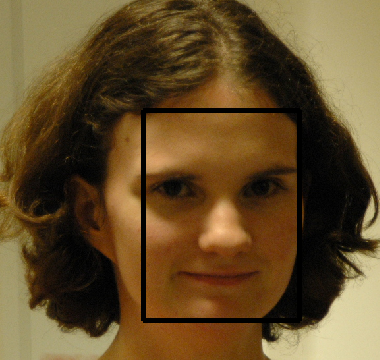
\includegraphics[height=\tempheight]{figures_pami/promo/case1/detector.png}&
\hspace{3mm}
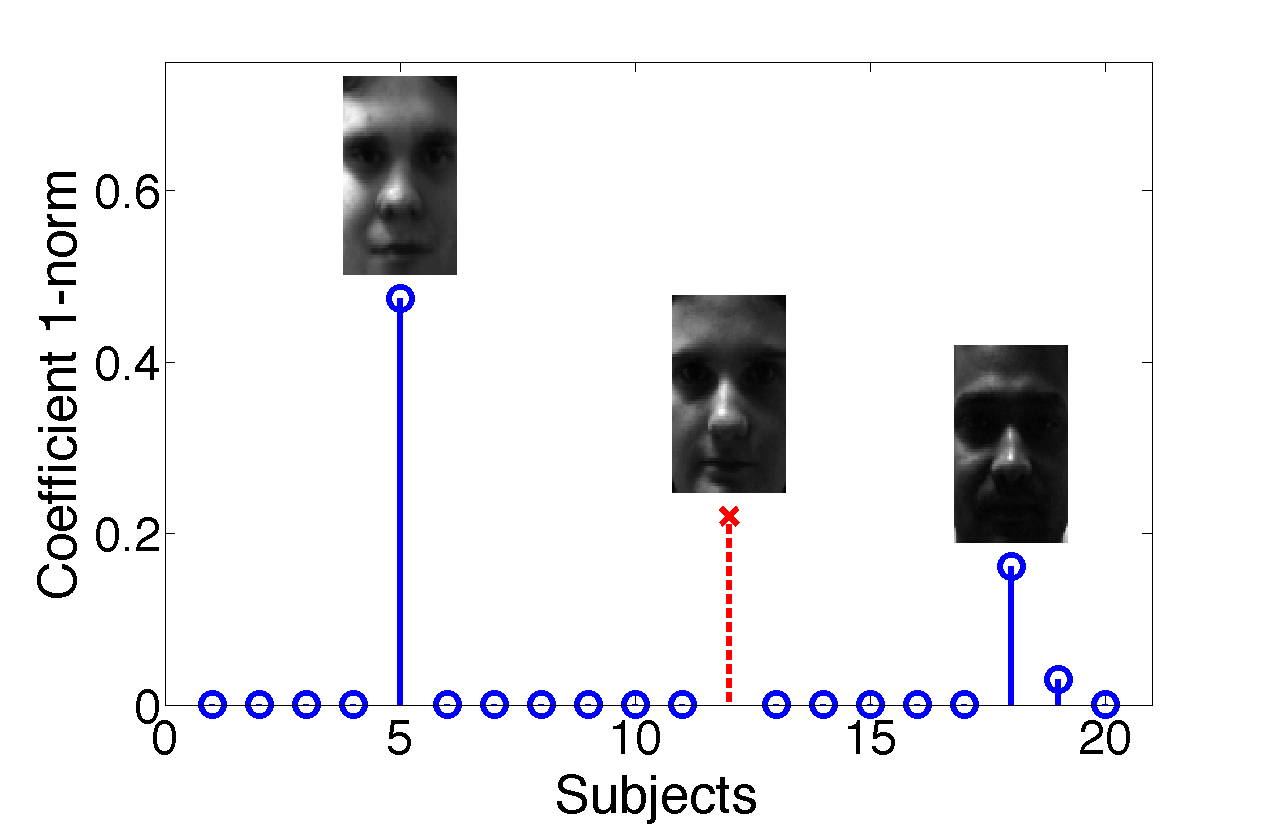
\includegraphics[height=\tempheight]{figures_pami/promo/case1/sci_with_axis_face_case1.png}
\\ 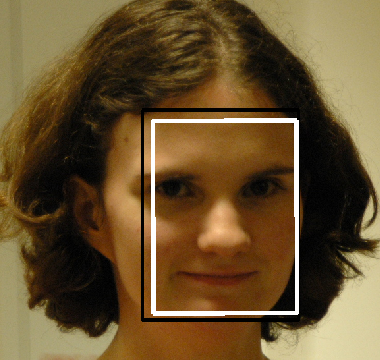
\includegraphics[height=\tempheight]{figures_pami/promo/alignment_and_detector.png}&
\hspace{3mm}
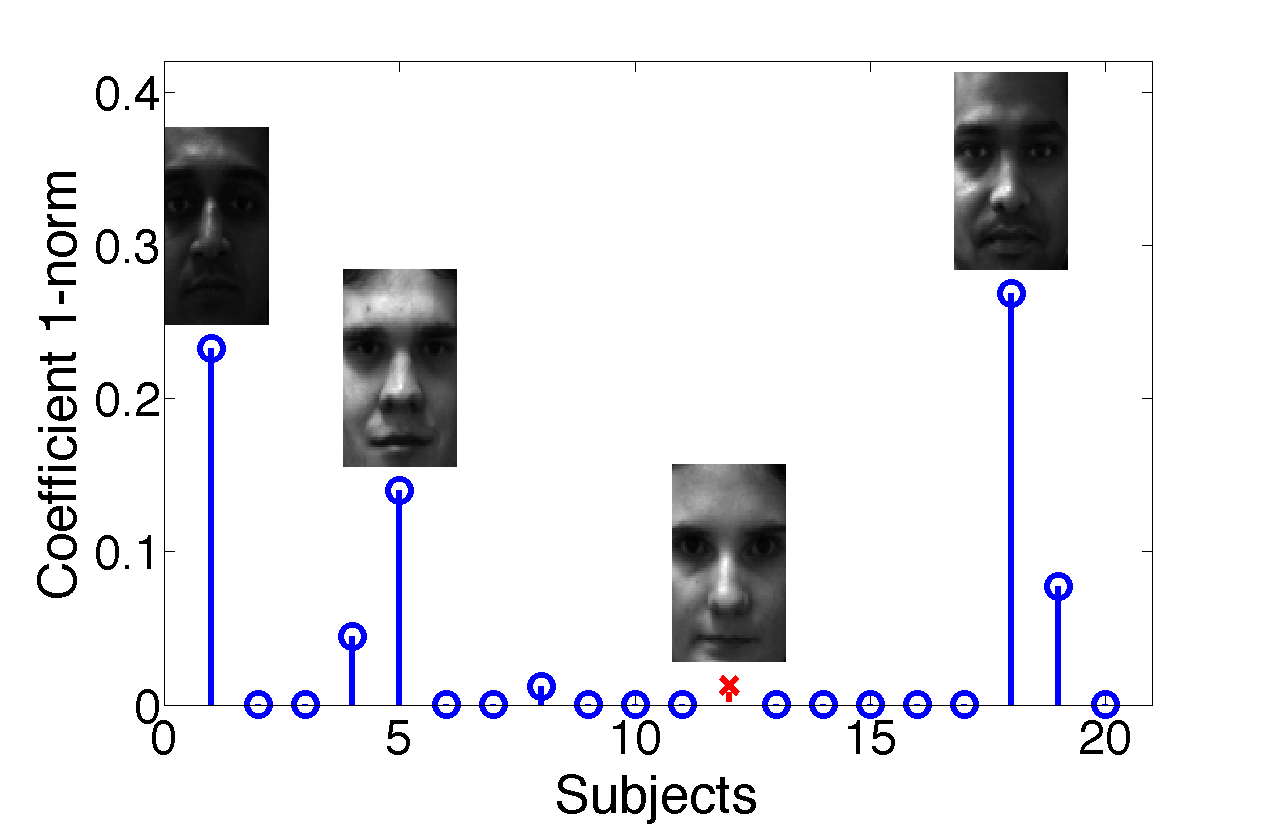
\includegraphics[height=\tempheight]{figures_pami/promo/case2/sci_with_axis_face_case2.png}
\\ 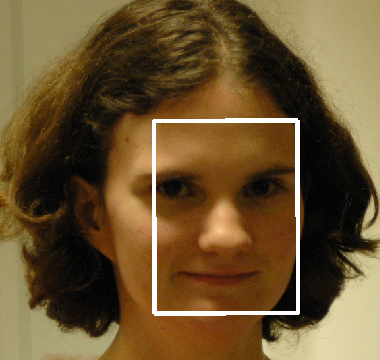
\includegraphics[height=\tempheight]{figures_pami/promo/case3/alignment.png} &
\hspace{3mm}
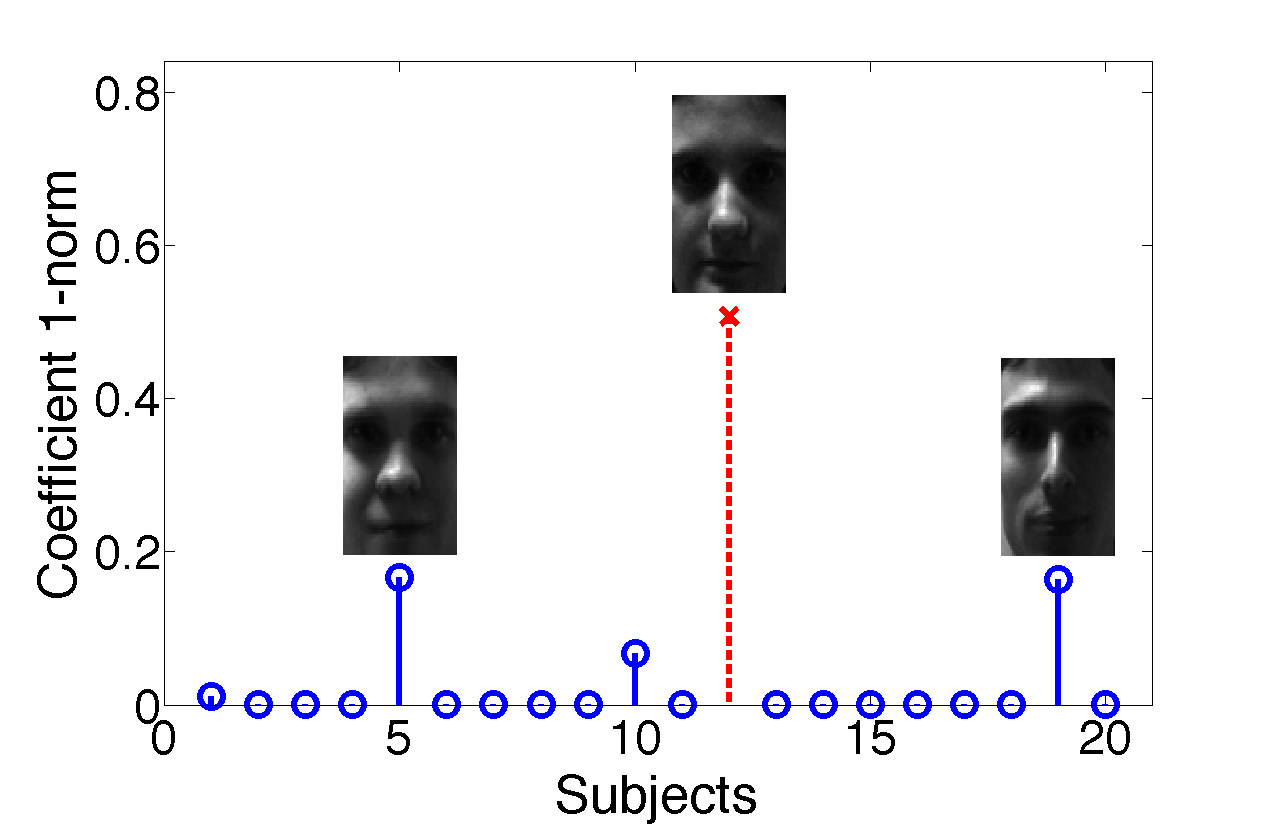
\includegraphics[height=\tempheight]{figures_pami/promo/case3/sci_with_axis_face_case3.png}
\end{tabular} \caption{\small{\bf Effects of registration and illumination on
Recognition}. In this example we identify the girl among 20 subjects, by
computing the sparse representation of her input face with respect to the
entire training set. The absolute sum of the coefficients associated with each
subject is plotted on the right. The weighted sum of the 
subject's training images using the associated sparse coefficients is also shown.
The red line (cross) corresponds to her true identity, subject 12. {\bf Top:} The
input face is from Viola and Jones' face detector (the black box) and all 38
illuminations specified in Section \ref{sec:illumination} are used in the
training.  {\bf Middle:} The input face is well-aligned (the white box) with
the training by our algorithm specified in Section \ref{sec:registration} but
only 24 frontal illuminations are used in the training for recognition (see
Section \ref{sec:illumination}). {\bf Bottom:} The input face is well aligned and
a sufficient set (all 38) of
illuminations are used in the training. Both are necessary for correct recognition
using SRC.}\label{fig:promo}
\end{figure}

\subsection{Relation to Earlier Work on Image Registration}

In holistic recognition algorithms (algorithms that use images themselves as
features) correspondence between points in the test image and in the gallery
images must be achieved.  A long line of research exists on using Active
Appearance Models \cite{Cootes2001-PAMI}, and the closely related Active Shape
Models \cite{cootes1992active} to register images against a relatively
high-dimensional model of plausible face appearances, often leveraging
face-specific contours.  While these model-based techniques have advantages in
dealing with variations in expression and pose, they may add unnecessary
complexity to applications where subjects normally present a neutral face or
only have moderate expression. Instead, this work focuses on classes of
deformations with far fewer degrees of freedom, i.e. similarity transformations
or perspective transformations.  Iterative registration in this spirit of this
work dates at least back to the Lucas-Kanade algorithm
\cite{lucas1981iterative}.

Whereas much of the early work on image registration is aimed at the problem of
registering nearly identical images, say by minimizing a sum of squared
distances or maximizing normalized correlation, face recognition applications
must confront several physical factors simultaneously: misalignment,
illumination variations, and corrupted pixels.  As will be discussed further
below, illumination variation can be dealt with by expressing the test image as
a linear combination of an appropriate set of training images. Similar
representations have been exploited in illumination-robust tracking (e.g.,
\cite{Belhumeur1999-PAA,Murase1995-IJCV}).  For robustness to gross errors, the
$\ell^1$-norm of the residual is a more appropriate objective function than the
classical $\ell^2$-norm. Its use here is loosely motivated by theoretical
results due to Cand\`{e}s and Tao \cite{CandesE2005-IT} (see also
\cite{Wright2008-IT}). These two observations motivate the reformulation of the
registration problem as the search for a set of transformations and
illumination coefficients that minimize the $\ell^1$-norm of the representation
error.  The proposed alignment system uses a generalized Gauss-Newton method
which solves a sequence of affine-constrained $\ell^1$-norm minimization
problems \cite{Osborne1990-JAMSSB,Jittorntrum1980-NM}. Each of these problems
can also be solved efficiently using recently developed first-order techniques
for $\ell^1$-minimization, which are reviewed in \cite{YangA2010-pp}.

% Illumination
Researchers have tried various techniques to deal with illumination variation.
In almost all recognition algorithms where only a single gallery image is
available per individual, illumination effects are regarded as a nuisance that
must be removed before the algorithm can continue.  This is typically done by
making statistical assumptions about how illumination affects the image, and
using those assumptions to extract a new representation that is claimed to be
illumination invariant.  Recent examples include \cite{chen2006total} and
\cite{zhou2007appearance}.  Despite these efforts, truly
illumination-invariant features remain difficult to obtain from a single input
image.  Clearly, if one has the luxury of designing the acquisition system
and the application demands a high recognition rate,
it is then unwise to limit the gallery to a
single image per person.  The proposed recognition system therefore takes the strategy of sampling many
gallery images of each individual under varying illuminations.  These images
are used as the basis for either a convex cone model
\cite{Georghiades2001-PAMI,belhumeur1998set}, or a subspace model
\cite{Basri2003-PAMI}.  Images are captured using a simple-to-construct
projector based light stage.  While similar systems have been used for
other applications, to our knowledge, this
system is the first to use projectors to indirectly illuminate a subject's face for
the purpose of face recognition.

\subsection{Contributions} This chapter demonstrates how registration and
illumination can be simultaneously addressed within a robust sparse
representation framework. Face registration, despite being a challenging
nonlinear problem, can be solved by a series of linear programs that
iteratively minimize the sparsity of the registration error. This leads to an
efficient and effective alignment algorithm for face images that works for a
large range of variation in translation, rotation, and scale, even when the
face is only partially visible due to eyeglasses, closed eyes and open mouth,
sensor saturation, etc.  A sufficient set of training illuminations that is
capable of linearly representing typical indoor and outdoor lighting is
determined empirically, and a practical hardware system based on synchronized
cameras and projectors is developed for capturing them.

%A key part of the system is exploiting
%an important property of the imaging process:  there is a linear mapping
%between the space of illuminations of an object, and the space of images of
%that object taken under the same pose.  This makes it possible to effectively
%model the testing image as a linear superposition of a large (and well chosen)
%set of training images.  This idea is certainly not new; indeed it has been in
%use for face recognition for roughly two decades, \cite{Turk1991-CVPR}.
%However, traditional algorithms that rely on this property of the image
%formation process have tended to perform very badly in the face of occlusions
%and when highly quality training images are unavailable.  

The chapter then demonstrates the effectiveness of the proposed new
methods with a complete face recognition system that is {\em
simple, stable, and scalable}. The proposed system performs
robust automatic recognition of subjects from loosely
controlled probe images taken both indoors and outdoors,
using a gallery of
frontal views of the subjects' faces under the proposed
illuminations. An off-the-shelf face
detector\footnote{We use the OpenCV
implementation of the Viola and Jones' face detector
\cite{Viola2004-IJCV}.} is used to detect faces in the test images.

Extensive experiments are conducted on the proposed system with
both public databases and a face database that is collected by
the proposed acquisition system. The experimental results on
large-scale public face databases show that the algorithm
indeed achieves very good performance on these databases,
exceeding or competing with the state-of-the-art algorithms.
Additionally, the experimental results on the private database
clearly demonstrate that the recognition system not only works well with
images taken under controlled laboratory conditions, but is
capable of handling practical indoor and outdoor illuminations as well.

\noindent{\em Organization of this chapter:} Section \ref{sec:registration},
presents a derivation of the robust registration and recognition algorithm within the sparse
representation framework. It further elaborates on algorithmic implementation issues,
conducts region of attraction experiments with respect to both 2D in-plane
deformation and 3D pose variation, and discusses its relationship to existing
work. Section \ref{sec:illumination} is dedicated to the training acquisition
system. This system is used to investigate empirically how many training
illuminations are required to handle practical illumination variations, and to
suggest a sufficient set of 38 training illuminations. Extensive experiments on
a large-scale public database and on a newly gathered database are conducted in Section
\ref{sec:multipie} and Section \ref{sec:own-data}, respectively, to verify the
proposed system. 

\section{Robust Alignment}\label{sec:registration} As demonstrated in Figure
\ref{fig:promo}(top), the main limitation of the {\em Sparse Representation and
Classification} (SRC) algorithm of \cite{Wright2009-PAMI} is the assumption of
pixel-accurate alignment between the test image and the training set. This
leads to brittleness under pose and misalignment, making it inappropriate for
deployment outside a laboratory setting. The goal of this section is to show
how this weakness can be rectified while still preserving the conceptual
simplicity and good recognition performance of SRC.

SRC assumes access to a database of multiple registered
training images per subject, taken under varying illuminations.
The images of subject $i$, stacked as vectors, form a matrix
$A_i \in \Re^{m \times n_i}$. Taken together, all of the images
form a large matrix $A = [ A_1 \mid A_2 \mid \dots \mid A_K ]
\in \Re^{m \times n}$. As argued in \cite{Wright2009-PAMI}, a
well-aligned test image $\y_0$ can be represented as a sparse
linear combination $A \x_0$ of all of the images in the
database,\footnote{This assumes that the training illuminations are sufficient. The next section will address how to ensure illumination
sufficiency.} plus a sparse error $\e_0$
due to corrupted pixels. The sparse representation can be recovered by
minimizing the $\ell^1$-norm\footnote{The $\ell^1$-norm of a
vector, denoted by $\|\cdot\|_1$, is the sum of absolute values of its entries.} of
$\x$ and $\e$:
\begin{equation}
\min_{\x,\e} \, \| \x \|_1 + \| \e\|_1 \quad \subj \quad \y_0 = A \x + \e.
\label{eqn:robust-l1}
\end{equation}
Now suppose that $\y_0$ is subject to some pose or
misalignment, so that instead of recording $\y_0$, the camera captures
a warped image $\y = \y_0 \circ \tau^{-1}$, for some
transformation $\tau \in T$ where $T$ is a finite-dimensional
group of transformations acting on the image domain.  The
transformed image $\y$ no longer has a sparse representation of
the form $\y = A \x_0 + \e_0$, and naively applying the
algorithm of \cite{Wright2009-PAMI} is no longer appropriate,
as seen in Figure \ref{fig:promo}(top).

\subsection{Batch and Individual Alignment} If the
true deformation $\tau^{-1}$ can be found, then
its inverse $\tau$ can be applied to the test image and it again becomes
possible to find a sparse representation of the resulting
image, as $\y \circ \tau = A \x_0 + \e_0$.\footnote{In the terminology of \cite{baker2004lucas}, this formulation is ``Forward Additive''.}
  This sparsity
provides a strong cue for finding the correct deformation
$\tau$: conceptually, one would like to seek a transformation
$\tau$ that allows the sparsest representation, via
\begin{equation} \label{eqn:L1-L1-conceptual}
\hat{\tau} = \arg\hspace{-2.5mm}\min_{\x,\e,\tau \in T} \| \x \|_1 + \| \e \|_1 \quad \subj \quad \y \circ \tau = A \x + \e.
\end{equation}
For fixed $\tau$, this problem is jointly convex in $\x$ and
$\e$. However, as a simultaneous optimization over the
coefficients $\x$, error representation $\e$, and
transformation $\tau$, it is a difficult, non-convex
optimization problem. One source of difficulty is the presence
of multiple faces in the matrix $A$:
\eqref{eqn:L1-L1-conceptual} has many local minima that
correspond to aligning $\y$ to different subjects. In this
sense, the misaligned recognition problem differs from the
well-aligned version studied in \cite{Wright2009-PAMI}. For the
well-aligned case, it is possible to directly solve for a
global representation, with no concern for local minima. With
possible misalignment, it is more appropriate to seek the best
alignment of the test face with each subject $i$:
\begin{equation} \label{eqn:per-subject-L1}
\hat \tau_i = \arg\hspace{-2.5mm}\min_{\x,\e,\tau_i \in T} \| \e \|_1 \quad \subj \quad \y \circ \tau_i = A_i \x + \e.
\end{equation}
It no makes sense to penalize $\| \x \|_1$, since $A_i$ consists of
only images of subject $i$ and therefore $\x$ is no longer expected to
be sparse.

\subsection{Alignment via Sequential $\ell^1$-Minimization} While the problem
\eqref{eqn:per-subject-L1} is still non-convex, for cases of practical interest
in face recognition, a good initial guess for the transformation is available,
e.g., from the output of a face detector. This initialization can be refined to
approach an estimate of the true transformation by repeatedly linearizing about  the
current estimate of $\tau$, and seeking representations of the form:
\begin{equation}
\y\circ \tau + J \Delta \tau = A_i \x + \e.
\end{equation}
Here, $J = \frac{\partial}{\partial \tau} \y \circ \tau$ is the Jacobian of $\y
\circ \tau$ with respect to the transformation parameters $\tau$, and $\Delta
\tau$ is the step in $\tau$. The above equation is under-determined if the
registration error $\e$ is allowed to be arbitrary. At the correct alignment it
is expected that the test image only differs from $A_i \x$ only for the
minority of the pixels corrupted by occlusions. Thus, the algorithm computes a
deformation step $\Delta \tau$ that best sparsifies the registration error
$\e$, in terms of its $\ell^1$-norm:
\begin{equation}
\Delta\hat{\tau}_1 = \arg\hspace{-3.5mm}\min_{\x,\e,\Delta\tau \in T} \| \e \|_1 \quad \subj \quad \y\circ\tau + J \Delta \tau = A_i \x + \e.
\label{eqn:L1-align}
\end{equation}
This is different from the popular choice that
minimizes the $\ell^2$-norm of the registration error:
\begin{equation}
\Delta\hat{\tau}_2 = \arg\hspace{-3.5mm}\min_{\x,\e,\Delta\tau \in T} \| \e \|_2 \quad \subj \quad \y\circ\tau + J \Delta \tau = A_i \x + \e,
\label{eqn:L2-align}
\end{equation}
which is also equivalent to finding the deformation step
$\Delta  \tau$ by solving the least-square problem:
$\min_{\x,\Delta \tau} \|\y \circ \tau + J\Delta \tau - A_i \x
\|_2$. Empirically, if there is only small noise
between $\y_0$ and $A_i\x$, both \eqref{eqn:L1-align} and
$\eqref{eqn:L2-align}$ have similar performance.  However, if
there are occlusions in $\y_0$, sequential
$\ell^1$-minimization \eqref{eqn:L1-align} is significantly
better than sequential $\ell^2$-minimization
\eqref{eqn:L2-align}. Figure \ref{fig:L1-L2-align} shows an
example.

The scheme \eqref{eqn:L1-align} can be viewed as a generalized Gauss-Newton
method for minimizing the composition of a non-smooth objective function (the
$\ell^1$-norm) with a differentiable mapping from transformation parameters to
transformed images. Such algorithms date at least back to the 1970's
\cite{Cromme1978-NM,Jittorntrum1980-NM}, and continue to attract attention
today \cite{Lewis2008-TR}. While a detailed discussion of their properties is
outside the scope of this thesis, it is worth mentioning that the scheme
\eqref{eqn:L1-align} is known to converge quadratically in the neighborhood of
any local optimum of the $\ell^1$-norm. In practice, this means that $\approx$
10 to 15 iterations suffice to reach the desired solution. The
interested reader is referred to \cite{Jittorntrum1980-NM,Osborne1990-JAMSSB} and the
references therein.

\renewcommand{\tempheight}[0]{1.0in}
\begin{figure}
\centering
{
\begin{tabular}{cccc}
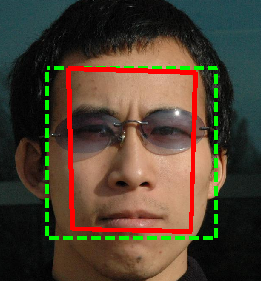
\includegraphics[height=\tempheight]{figures_pami/L1_cropped} &
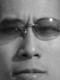
\includegraphics[height=\tempheight]{figures_pami/y_warp_L1} &
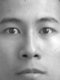
\includegraphics[height=\tempheight]{figures_pami/y_hat_L1} &
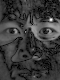
\includegraphics[height=\tempheight]{figures_pami/e_L1} \\
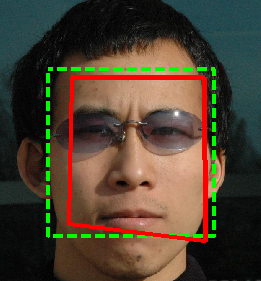
\includegraphics[height=\tempheight]{figures_pami/L2_cropped} &
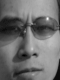
\includegraphics[height=\tempheight]{figures_pami/y_warp_L2} &
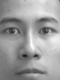
\includegraphics[height=\tempheight]{figures_pami/y_hat_L2} &
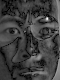
\includegraphics[height=\tempheight]{figures_pami/e_L2} \\
(a) & (b) & (c) & (d)
\end{tabular}}
\caption{\small{\bf Comparing alignment of a subject wearing sunglasses by
$\ell^1$ and $\ell^2$ minimization.}
{\bf Top:} alignment result of minimizing $\|\e\|_1$; {\bf Bottom:}
result of minimizing $\|\e\|_2$. (a) {\em Green (dotted):} Initial face boundary
given by the face detector, {\em Red (solid):} Alignment result shown on the same
face; (b) warped testing image using the estimated transformation $\y_0$;
(c) reconstructed face $A_i\x$ using the training; (d) image of error $\e$. }\label{fig:L1-L2-align}
\end{figure}

In addition to normalizing the training images (which is done
once), it is important to normalize the warped testing image
$\y \circ \tau$ as the algorithm runs.  Without normalization,
the algorithm may fall into a degenerate global minimum
corresponding to zooming in on a dark region of the test
image.  Normalization is done by replacing the linearization of
$\y \circ \tau$ with a linearization of the normalized version
$\tilde \y(\tau) = \frac{\y \circ \tau}{\|\y \circ \tau\|_2}$.
The proposed alignment algorithm can be easily extended to work
in a {\em multiscale} fashion, with benefits both in
convergence behavior and computational cost.  The alignment
algorithm is simply run to completion on progressively less
downsampled versions of the training and testing images, using
the result of one level to initialize the next.

\subsection{Robust Recognition by Sparse Representation} Once
the best transformation $\tau_i$ has been computed for each
subject $i$, the training sets $A_i$ can be aligned to $\y$,
and a global sparse representation problem of the form
\eqref{eqn:robust-l1} can be solved to obtain a discriminative
representation in terms of the entire training set. Moreover,
the per-subject alignment residuals $\| \e \|_1$ can be used to
prune unpromising candidates from the global optimization,
leaving a much smaller and more efficiently solvable problem.
The complete optimization procedure is summarized as Algorithm
\ref{alg:deformable-src}. The parameter $S$ is the number of subjects
considered together to provide a sparse representation for the
test image. If $S = 1$, the algorithm reduces to classification
by registration error; but considering the test image might be
an invalid subject, $S=10$ is typically chosen. Since valid
images have a sparse representation in terms of this larger
set, invalid test images can be rejected using the {\em sparsity
concentration index} proposed in \cite{Wright2009-PAMI}.
The function $\delta_i(\x)$ in Algorithm \ref{alg:deformable-src}
selects coefficients from the vector $\x$ corresponding to subject $i$.

Another important free parameter in Algorithm \ref{alg:deformable-src} is the
class of deformations $T$. In the experiments presented here, 2D similarity
(i.e. 2D rigid transformations) transformations are used, $T =
\mathbb{SE}(2)\times \Re_+$\footnote{Here, SE stands for Special Euclidean.
The $\Re_+$ accounts for the scale.}, for removing alignment error incurred by
face detector, or 2D projective transformations, $T =
\mathbb{GL}(3)\footnote{Here, GL stands for General Linear.  This class of
transformations is able to represent distortion in a perspective image of a
planar object.}$, for handling some pose variation.

Algorithm \ref{alg:deformable-src}, also implements a simple heuristic
motivated by the observation that the face detector output may be poorly
centered on the face and may contain a significant amount of the background:
before the recognition stage, instead of aligning the training sets to the
original $\y$ directly obtained from the face detector, the transformations of
the top $S$ classes $\tau_{k_1}, \tau_{k_2}, \ldots, \tau_{k_S}$ are averaged
into a transformation $\bar{\tau}$.  Updating $\y$ according to $\bar{\tau}$
results in a better centered test image. For the 2D similarity transformations,
which are used in our system when initialized by the face detector, a
transformation $\tau$ can be parameterized as $\tau = (\tau^1, \tau^2, \tau^3,
\tau^4)$, where $\tau^1$ and $\tau^2$ represent the translations in $x$- and
$y$-axis, $\tau^3$ represents the rotation angle and $\tau^4$ represents the
scale. The average transformation is simply obtained by taking the
component-wise mean:
\begin{displaymath}
\bar{\tau}^i = (\tau_{k_1}^i + \tau_{k_2}^i + \cdots +
\tau_{k_S}^i) / S, i = 1,2,3,4.
\end{displaymath}
Finally, the training sets are aligned to the new $\y$.

\begin{algorithm}[thb]
\caption{\bf\small (Deformable Sparse Recovery and Classification for
Face Recognition)} \label{alg:deformable-src}
\begin{algorithmic}[1]
\begin{small}
\STATE {\bf Input:} Training images $\{A_i \in \Re^{m\times n_i}\}_{i=1}^K$ for $K$ subjects,  a test image
$\bb\in\Re^m$ and a deformation group $T$.
\STATE
{\bf for} each subject $i$,
\STATE \hspace{3mm} $\tau^{(0)}
\leftarrow I$.
\STATE \hspace{3mm} {\bf while} not converged $(j=1,2,\ldots)$ {\bf do}
\STATE \hspace{6mm}
$\tilde \bb(\tau) \leftarrow \frac{\bb \circ \tau}{\|\bb \circ
\tau\|_2}$; \;\;\; $J \leftarrow  \frac{\partial}{\partial
\tau} \tilde\bb(\tau)  \bigr|_{\tau^{(j)}} $;
%\STATE \hspace{6mm} $(\hat \x, \hat \e, \Delta \tau) \leftarrow \left\{\begin{array}{l} \arg \min_{\x,\e,\Delta \tau} \| \e \|_1 \\  \subj \; \bb + J \Delta \tau = A_k \x + \e \end{array}\right.$
\STATE \hspace{6mm} $ \Delta \tau =  \arg\min \; \| \e \|_1  \;
\subj \; \tilde \bb + J \Delta \tau = A_i \x + \e.$
\STATE
\hspace{6mm} $\tau^{(j+1)} \leftarrow \tau^{(j)} + \Delta
\tau$;
\STATE \hspace{3mm} {\bf end while} \STATE {\bf end} \STATE Keep
the top $S$ candidates $k_1, \ldots, k_S$ with the smallest
residuals $\|\e\|_1$. \STATE Compute an average transformation
$\bar{\tau}$ from $\tau_{k_1}, \tau_{k_2}, \ldots, \tau_{k_S}$.
\STATE Update $\bb \leftarrow \bb \circ \bar{\tau}$ and $\tau_i
\leftarrow \tau_i \cdot \bar{\tau}^{-1}$ for $i = k_1, \dots,
k_S$. \STATE Set $A \leftarrow \big[ A_{k_1} \circ
\tau_{k_1}^{-1} \mid A_{k_2} \circ \tau_{k_2}^{-1} \mid \dots
\mid A_{k_S} \circ \tau_{k_S}^{-1} \big]$. \STATE Solve the
$\ell_1$-minimization problem: \\
\hspace{2em}$\hat{\x} = \arg \min_{\x, \e} \| \x \|_1 + \|\e\|_1 \;\; \subj \;\; \bb = A \x + \e.$
\STATE Compute residuals $r_i(\bb) = \| {\bb} - {A}_i \, \delta_i(\hat{\x}) \|_2$ for $i = k_1, \dots, k_S$.
\STATE {\bf Output:} $\mbox{identity}(\bb) = \arg\min_i r_i(\bb)$.
\end{small}
\end{algorithmic}
\end{algorithm}
%\vspace{-4mm}


The transformation $\tau$ defines a mapping between the coordinates of pixels
in the large original image and a smaller (un)warped image. The pixels of the
small image are stacked into a vector. To prevent aliasing artifacts in the
downsampled image, it is necessary to apply a smoothing filter to the original
image beforehand. For a simple implementation, a rectangular window with
regular sampling can used, but in general, the small image need not be
regularly sampled in pixel coordinates.  For example, the sample locations
could be arbitrarily selected from within a ``face shaped'' area. The impact of
non-rectangular sampling windows on performance of the algorithm will be
discussed in Section \ref{sec:multipie}.

\subsection{System Implementation}
The runtime of Algorithm~\ref{alg:deformable-src} is dominated
by the time spent solving two qualitatively similar $\ell_1$ minimization problems.
Custom $\ell_1$ minimization solvers for this purpose based on
\emph{Augmented Lagrange Multiplier} (ALM) algorithm have been developed.
the ALM algorithm was selected because it strikes the best
balance between speed, accuracy, and scalability.  Several $\ell_1$ minimization
algorithms were tested for the face recognition problem, 
and ALM was found to have the best performance. 
A more in-depth discussion of the solvers will be presented
in Chapter \ref{chap:minimization}
For a more detailed discussion of competing
approaches, the interested reader is referred to
\cite{YangA2010-pp}.
On a Mac Pro with
two Dual-Core 2.66GHz Xeon processors and 4GB memory,
running on a private database containing images size $80\times 60$
pixels from 109 subjects under 38 illuminations,
the C++ implementation of Algorithm~\ref{alg:deformable-src} takes
about 0.60 seconds per subject for alignment and about 2.0
seconds for global recognition. Compared to the highly
customized interior point method first presented in 
\cite{Wagner2009-CVPR}, this new algorithm is
only slightly faster for per subject alignment. However, it is
much simpler to implement and it achieves a
\emph{speedup of more than a factor of 10} for global
recognition!  Performance optimization of this algorithm
will be discussed in Chapter \ref{chap:parallel}.

\subsection{Experiments on Region of Attraction} Three experimental results
will now be presented to demonstrate the effectiveness of the individual
alignment procedure outlined in the previous section. They show sufficiency of
the region of attraction, verify effectiveness of the multiscale extension, and
show stability to small pose variations.  After a discussion of illumination
invariance in the next section, large-scale recognition experiments are
presented in Sections \ref{sec:multipie} and \ref{sec:own-data}.

\noindent {1) \em 2D Deformation.}  The first experiment verifies the
    effectiveness of our alignment algorithm with images
    from the CMU Multi-PIE Database \cite{Gross2008-FGR}.
    The gallery set consists of all the subjects in Session 1, using 7
    illuminations per person. The test images use
    one new illumination from each user in Session
    2.\footnote{The training are illuminations $\{0, 1, 7,
    13, 14, 16, 18\}$ of \cite{Gross2008-FGR}, and the
    testing is the illumination 10. } A ground truth for
	registration is formed by manually selecting
    eye corners in both training and testing images. 
	The images are downsampled to a canonical image size of 
    $80\times 60$ pixels\footnote{Unless otherwise stated,
    this will be the default resolution at which 
    all training and testing datasets are resampled.} 
	and the distance between the two outer
    eye corners is normalized to be 50 pixels for each
    person. An artificial deformation is applied to the
    testing image with a combination of translation,
    rotation and scaling. A small value for the alignment
    error $r = \|\e\|_1$ is chosen as an indicator of success. Let $r_0$
    be the alignment error obtained by aligning a test
    image to the training images without any artificial
    perturbation. After the test image is artificially
    perturbed and aligned resulting in an alignment error
    $r$, we consider the alignment successful if $|r - r_0 | \leq
    0.01r_0$. Figure \ref{fig:attraction} shows the
    percentage of successful registrations for all subjects
    for each artificial deformation. The results suggest
    that the alignment algorithm works extremely well with
    translation up to 20\% of the eye distance (or 10
    pixels) in all directions and up to $30^\circ$ in-plane
    rotation. Tests of the alignment algorithm
    with scale variation show that it can handle up to 15\%
    change in scale.

In order to determine if this region of attraction is sufficient,
it must be compared to the accuracy achieved by the initialization
provided by the face detector.  Statistics of the Viola and Jones'
 face detector on the Multi-PIE dataset. For 4,600 frontal
 images of 230 subjects under 20 different illuminations,
 using manual registration as the ground truth, the average
 misalignment error of the detected faces is about 6 pixels
 and the average variation in scale is 8\%. This falls
 safely inside the region of attraction for our alignment
 algorithm.
\newcommand{\tempheighta}[0]{1.1in}
\newcommand{\tempheightb}[0]{0.9in}
\begin{figure*}
\centering
{
\begin{tabular}{ccc}
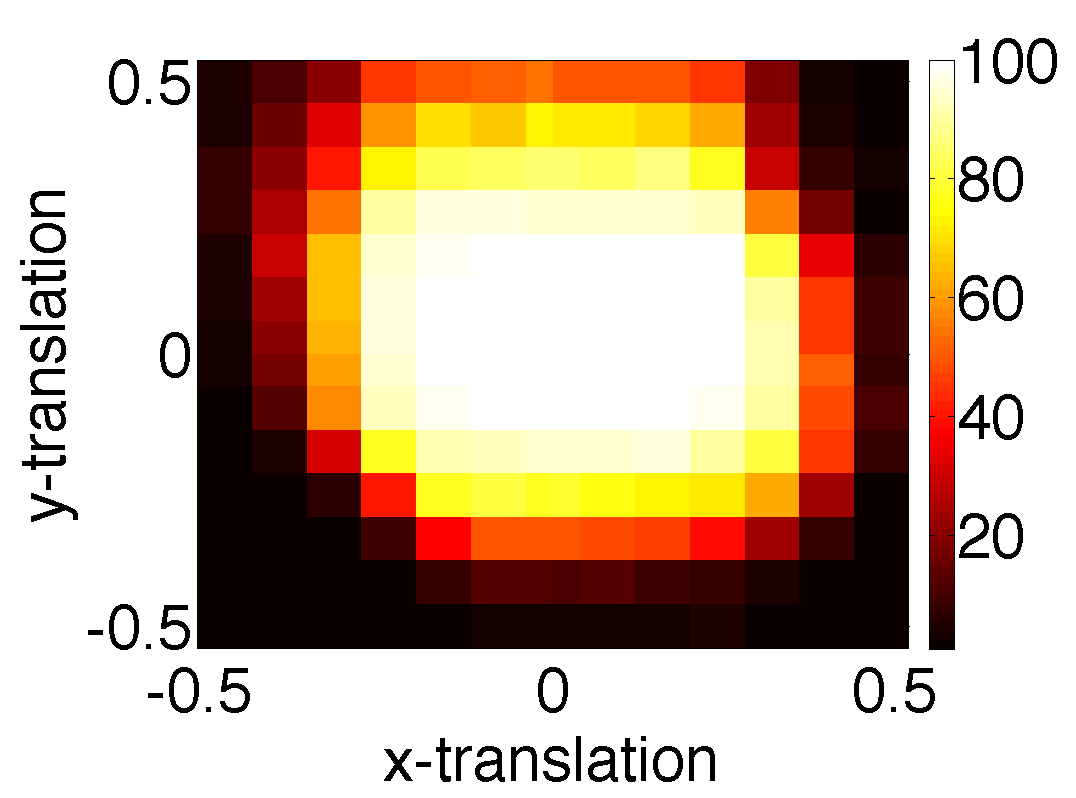
\includegraphics[height=\tempheighta]{figures_pami/x_y_roa.png} &
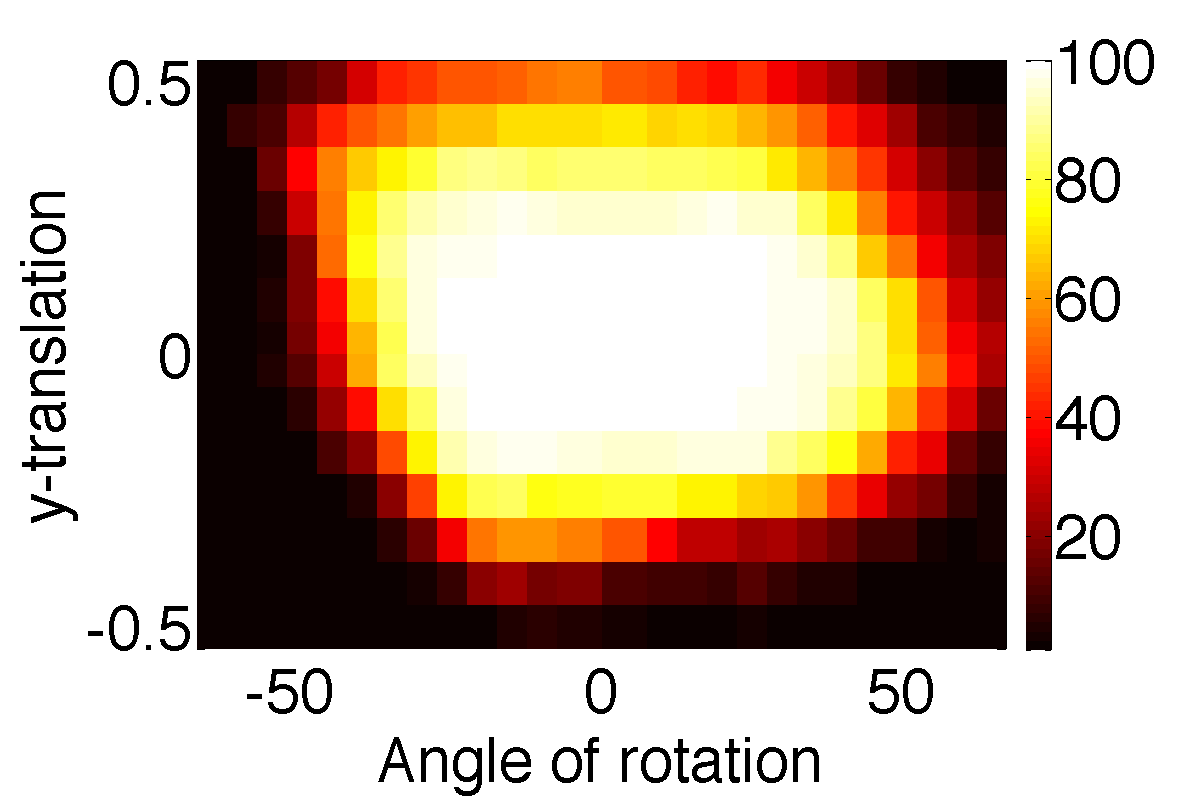
\includegraphics[height=\tempheighta]{figures_pami/y_theta_roa.png} &
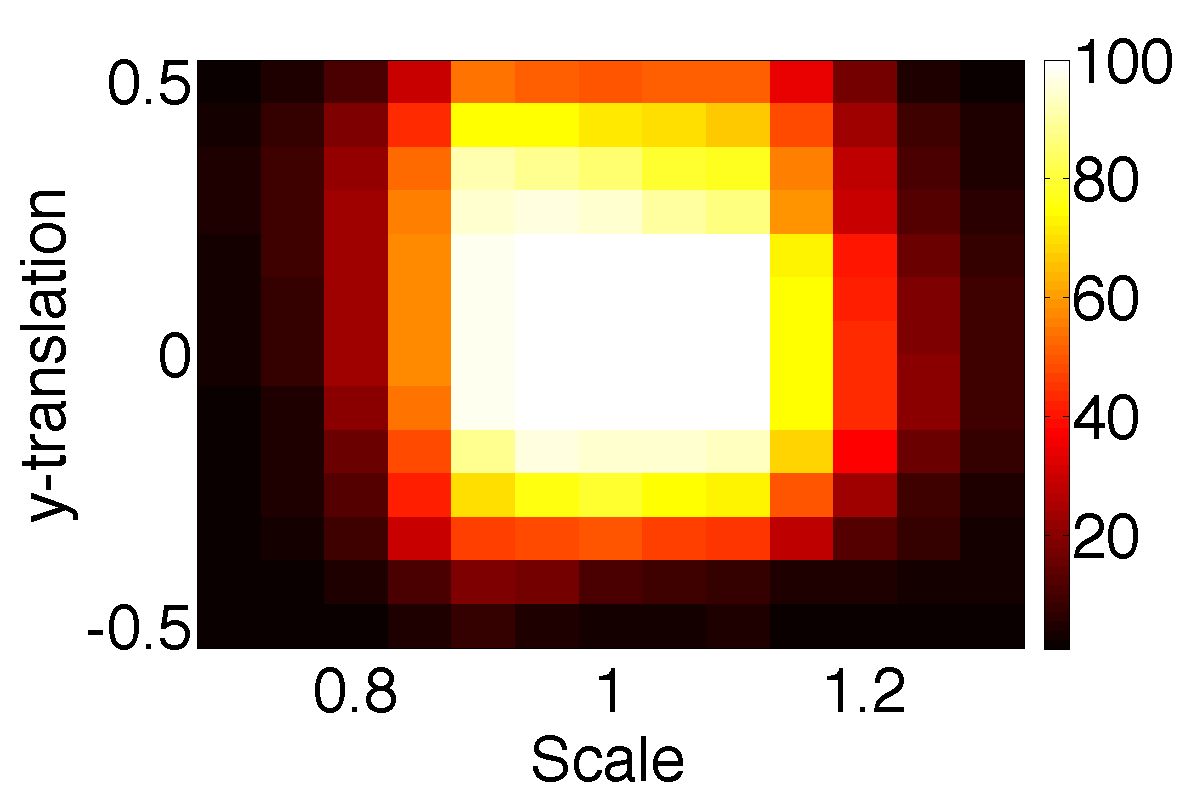
\includegraphics[height=\tempheighta]{figures_pami/y_s_roa.png}\\
(a)&(b)&(c)
\end{tabular}
\begin{tabular}{cccc}
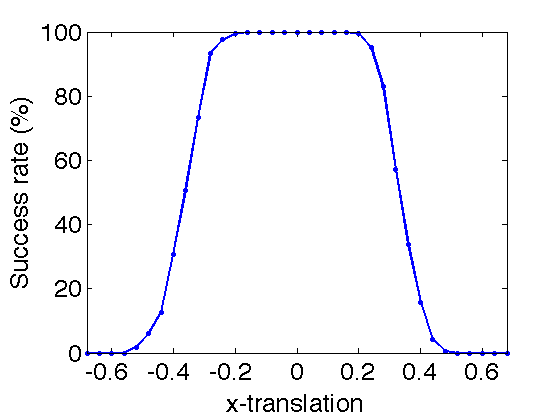
\includegraphics[height=\tempheightb]{figures_pami/x_tr.png} &
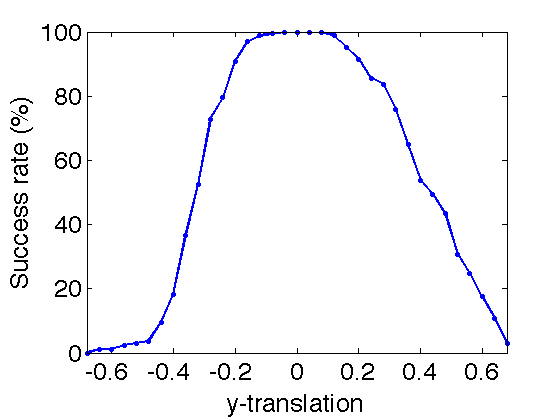
\includegraphics[height=\tempheightb]{figures_pami/y_tr.png} &
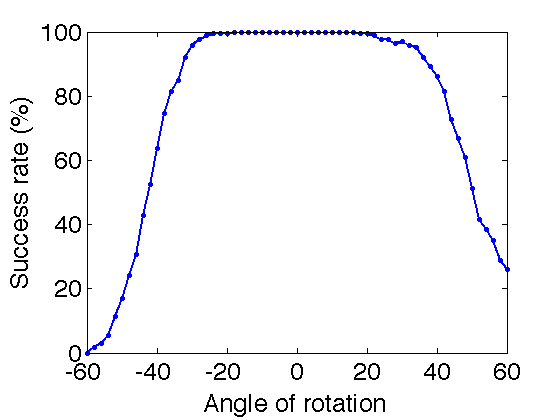
\includegraphics[height=\tempheightb]{figures_pami/theta.png} &
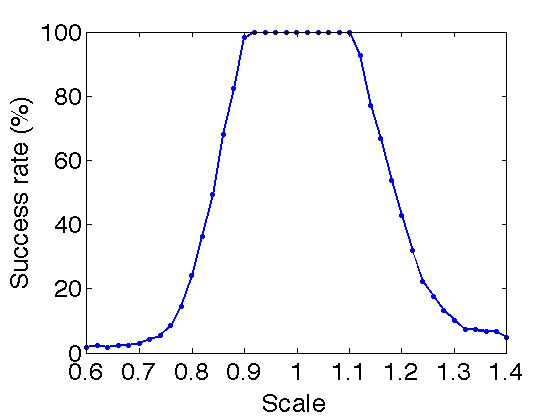
\includegraphics[height=\tempheightb]{figures_pami/scale.png}\\
(d)&(e)&(f)& (g)
\end{tabular}
} \caption{\small{\bf Region of attraction.} Fraction of
subjects for which the algorithm successfully aligns a
synthetically perturbed test image.  The amount of translation
is expressed as a fraction of the distance between the outer
eye corners, and the amount of in-plane rotation in degrees.
{\bf Top row:} (a) Simultaneous translation in $x$ and $y$
directions. (b) Simultaneous translation in $y$ direction and
in-plane rotation. (c) Simultaneous translation in $y$
direction and scale variation. {\bf Bottom row:} (d)
Translation in $x$ direction only. (e) Translation in $y$
direction only. (f) In-plane rotation only. (g) Scale variation
only.} \label{fig:attraction} 
\end{figure*}

\noindent{2) \em Multiscale Implementation.}
Performing alignment in a multiscale fashion has two benefits: first, it provides a larger region of attraction, and second, it reduces overall computational cost. Here, we further investigate the convergence behavior of the algorithm as a function of the standard deviation $\sigma$ of the Gaussian smoothing filter and the number of scales considered.
We use the same 7 illuminations in
Session 1 as training, and all 20 illuminations in the same
session as testing. We introduce artificial deformation in
both $x$ and $y$ directions up to 16 pixels in the
$80\times 60$ frame, with a step size of 4 pixels, i.e.,
$(\Delta x, \Delta y) \in \{-16,-12,\ldots,12,16\} \times
\{-16,-12,\ldots,12,16\}$. We consider an alignment
successful if the estimated coordinates of the eye-corners
are within 1 pixel from the ground truth in the original
image.  In Figure \ref{fig:multiscale}, we report the
alignment success rate, averaged over the artificially
perturbed initial deformations, as a function of the
standard deviation of the Gaussian kernel $\sigma$, for
three choices of the number of scales. As one can see,
using multiscale indeed improves the performance, and when
3 scales are used, a smaller convolution kernel can achieve
a similar performance compared to a much larger kernel when
only 2 scales are used.
\begin{figure}
\centering
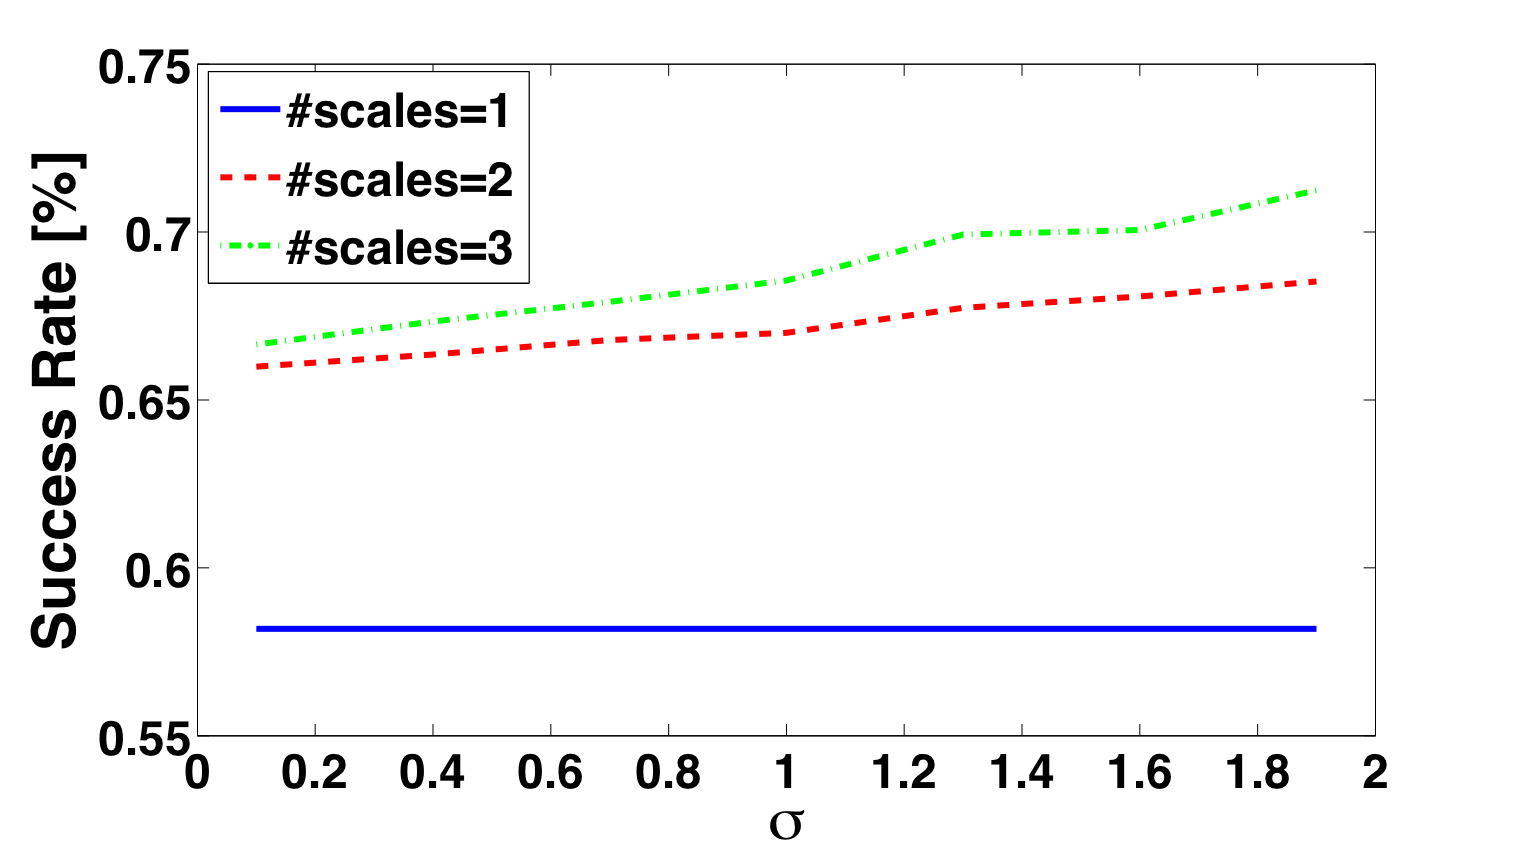
\includegraphics[width=4in]{figures_pami/multiscale.png}
\caption{\small{\bf Multiscale alignment.} This figure shows the average success rate of alignment over all possible perturbations. A smaller blur kernel can be applied to achieve certain level of performance when more scales are used.}
\label{fig:multiscale}
\end{figure}

\noindent{3) \em 3D Pose Variation.} As densely sampled pose
and
    illumination face images are not available in any of
    the public databases, including Multi-PIE, we have
    collected our own dataset using our own system (to be
    introduced in the next section). We use frontal face
    images of a subject under the 38 illuminations proposed
    in the next section as training. For testing, we
    collect images of the subject under a typical indoor
    lighting condition at pose ranging from $-90^\circ$ to
    $+90^\circ$ with step size 5.625$^\circ$, a total of 33
    poses. We use Viola and Jones' face detector to
    initialize our alignment algorithm.
Figure \ref{fig:pose-alignment} shows that our algorithm works reasonably well with poses up
to $\pm 45^\circ$.
Note that this level of out-of-plane
 pose variation is beyond what we intend to handle with our formulation.
\begin{figure}
\centering
{
\begin{tabular}{ccccc}
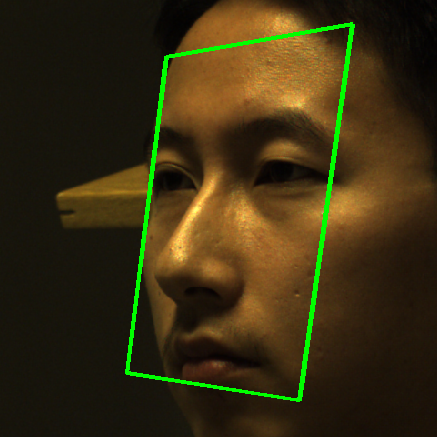
\includegraphics[height=1in]{figures_pami/5} &
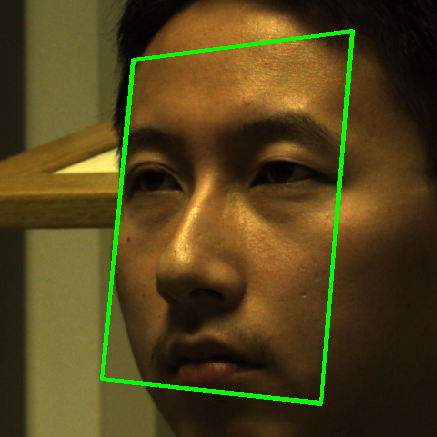
\includegraphics[height=1in]{figures_pami/7} &
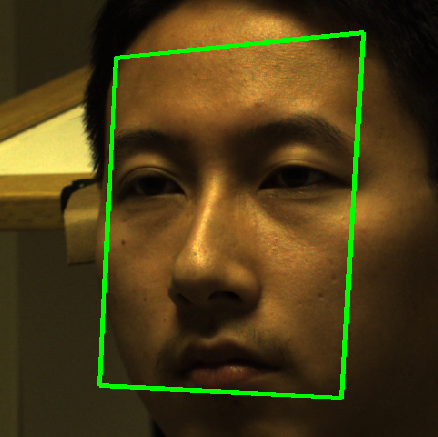
\includegraphics[height=1in]{figures_pami/09} &
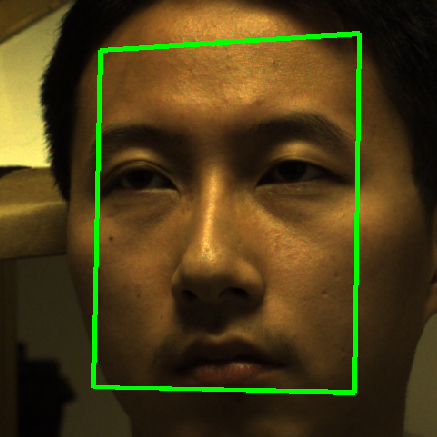
\includegraphics[height=1in]{figures_pami/11} &
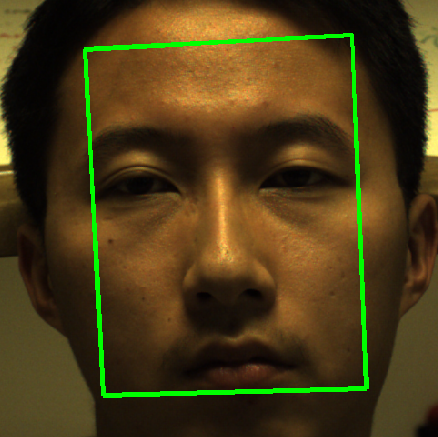
\includegraphics[height=1in]{figures_pami/13} \\
(a) & (b) & (c) & (d) & (e)\\
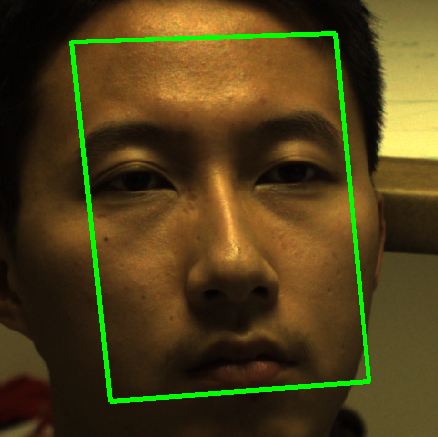
\includegraphics[height=1in]{figures_pami/15} &
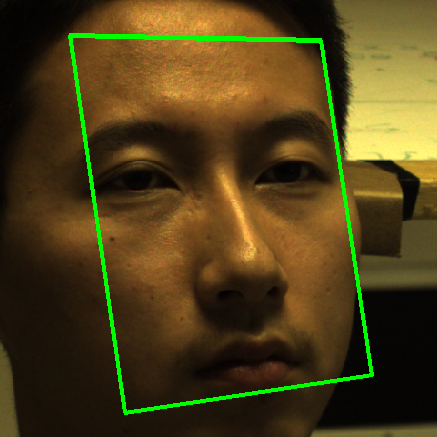
\includegraphics[height=1in]{figures_pami/17} &
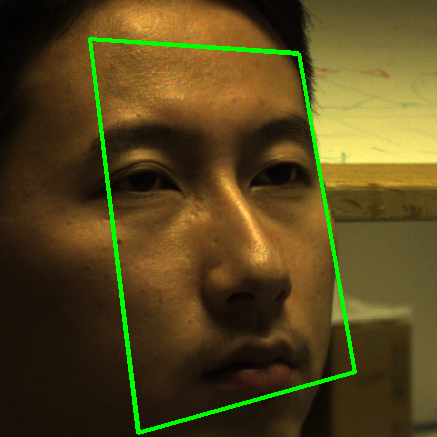
\includegraphics[height=1in]{figures_pami/19} &
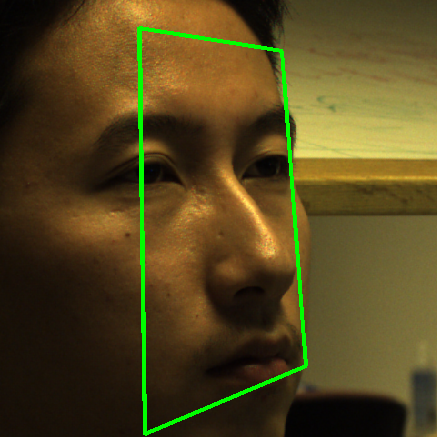
\includegraphics[height=1in]{figures_pami/21} &
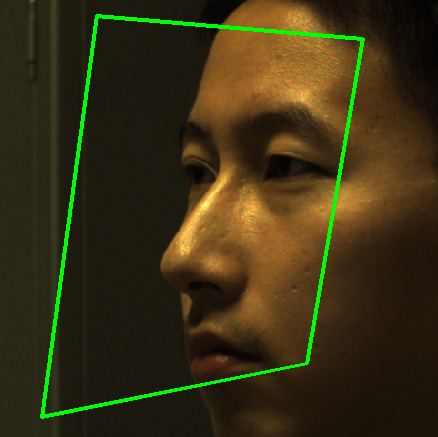
\includegraphics[height=1in]{figures_pami/3} \\
(f) & (g) & (h) & (i) & (j)
\end{tabular}
}
\caption{\small{\bf 2D Alignment of test images with different poses to frontal training images.} {\bf (a) to (i):}  plausible alignment for pose from $-45^{\circ}$
to $+45^{\circ}$. {\bf (j):} a case when the algorithm fails for an extreme pose ($>45^{\circ}$).
}\label{fig:pose-alignment} 
\end{figure}
\subsection{Comparison with Related Work}
Our modification to SRC roots solidly in the tradition of
adding deformation-robustness to face recognition algorithms
\cite{Cootes2001-PAMI,Gross2006-PAMI,Wiskott1997-PAMI}.
However, the only previous work to investigate face alignment
in the context of sparse signal representation and SRC is the
work of \cite{Huang2008-CVPR}. They consider the case where the
training images themselves are misaligned and allow one
deformation per training image. They linearize the training
rather than the test, which is computationally more costly as
it effectively triples the size of the training set. In
addition, as they align the test image to all subjects
simultaneously, it potentially is more prone to local minima
when the number of subjects increases, as we will see in the
following experimental comparisons.
\begin{enumerate}
\item {\em Extended Yale B.} In this experiment, we have
    used the same experimental settings as in
    \cite{Huang2008-CVPR}. 20 subjects are selected and
    each has 32 frontal images (selected at random) as
    training and another 32 for testing. An artificial
    translation of 10 pixels (in both $x$ and $y$
    directions) is introduced to the test image. For our
    algorithm we downsample all the images to $88\times
    80$ for memory reasons, whereas the work of
    \cite{Huang2008-CVPR} uses random projections.
Note that the use of cropped images in this experiment introduces image boundary effects.
    Our
    algorithm achieves the recognition rate 93.7\%,
    compared to 89.1\% recognition rate reported in
    \cite{Huang2008-CVPR}.
\item {\em CMU Multi-PIE.} In this experiment, we choose
    all subjects from the CMU Multi-PIE database, 7
    training images from Session 1 and 1 test image from
    Session 2 per person. The setting is exactly the same
    as the previous experiment on 2D deformation. We again
    work with downsampled images of size $80\times 60$ pixels. An
    artificial translation of 5 pixels (in both $x$ and $y$
    directions) was induced in the test image. The
    algorithm of \cite{Huang2008-CVPR} achieves a
    recognition rate of 67.5\%,\footnote{That algorithm has
    two free parameters - $l$ and $d$, which govern the tradeoff between
	accuracy and run-time. For this experiment
    we chose $l = 1$ and $d = 514$.} while ours achieves 92.2\%.
    \end{enumerate}
				
\section{Handling Illumination Variation}\label{sec:illumination}
In the above section, we have made the assumption that the test image, although taken under some arbitrary illumination, can be linearly represented by a finite number of training illuminations.  Under what conditions is this a reasonable assumption to make?  What can we say from first principles about how the training images should be chosen?

\subsection{The Illumination Model}

The strongest theoretical results so far regarding the relationship
between illumination and the resulting sets of images is due to Basri and Jacobs \cite{Basri2003-PAMI}.
The main result of this section is that for convex Lambertian objects, distant illuminations, and fixed pose,
all images of the object can be well approximated by linear combinations of
nine (properly chosen) basis images.  The basis images have mixed sign, and
their illuminations consist of the lowest frequency spherical harmonics.
While this is a very important result for understanding the image
formation process, the direct application of this result in most practical
systems is misguided for several reasons.
Specularities, self-shadowing, and inter-reflections all dramatically affect the appearance of face images,
and they all do so in a way that violates the modeling assumptions of the Basri analysis.

Fortunately, even with these effects, for most materials the relationship between
illumination and image is still linear,\footnote{Materials that break
this assumption include fluorescent materials and the photochromic (``Transition'') lenses
in some eyeglasses.  Most materials emit light in proportion to their
incident light.} provided the sensor has a linear response curve.\footnote{Proper handling of gamma encoding is an important consideration for
practitioners.  Most cameras apply a non-linear and often undocumented response
curve to captured images.  A slight degradation of performance will occur if
gamma compressed images are treated as if they were linear.  We recommend the use
of cameras with well documented response curves that can be inverted when the
image file is loaded.}
For a more in-depth study
of the relationship between illumination and images, we refer the reader to
\cite{belhumeur1998set}.
While the relationship between illuminations and images is linear,
only positive weights are allowed; the space of all images of an object with
fixed pose and varying illumination is a convex cone lying in the positive
orthant. The question becomes, how many images does it take to do a good job
of representing images sampled from this cone?

It has been observed in various empirical studies that
one can get away with using a small number of frontal
illuminations to linearly represent a wide range of new frontal
illuminations, when they are all taken under the same laboratory conditions
\cite{Georghiades2001-PAMI}. This is the case for many public
face datasets, including AR, ORL, PIE, and Multi-PIE.
Unfortunately, we have found that in practice, a training
database consisting purely of frontal illuminations is not
sufficient to linearly represent images of a faces taken
under typical indoor or outdoor conditions (see the experiment
conducted in Section \ref{sec:own-data}). As illustrated by the
example in Figure \ref{fig:promo}, an insufficient number of
training illuminations can result in recognition failure. To
ensure our algorithm works in practice, we need to find a set
of training illuminations that are indeed {\em sufficient} to
linearly represent a wide variety of practical indoor and
outdoor illuminations.


\subsection{Projector-based Illumination System}

We have designed a system that can acquire frontal images of a subject while
simultaneously illuminating the subject from all directions above horizontal. A sketch of the
system is shown in Figure \ref{fig:system}: The illumination
system consists of four projectors that display various bright
patterns onto the three white walls in the corner of a dark
room.  The light reflects off of the walls and illuminates the
user's head indirectly.  After taking the frontal illuminations
we rotate the chair by 180 degrees and take pictures from the
opposite direction.  Having two cameras speeds the process
since only the chair needs to be moved in between frontal and
rear illuminations. Our projector-based system has several
advantages over flash-based illumination systems for face recognition:
\begin{itemize}
\item The illuminations can be modified in software, rather than hardware.
\item It is easy to capture many different illuminations quickly.
\item Good coverage and distant illumination can be achieved simultaneously.
\item There is no need to mount anything on the walls or construct a large dome.
\item The system can be assembled from off-the-shelf hardware.
\end{itemize}
\begin{figure}
\centering
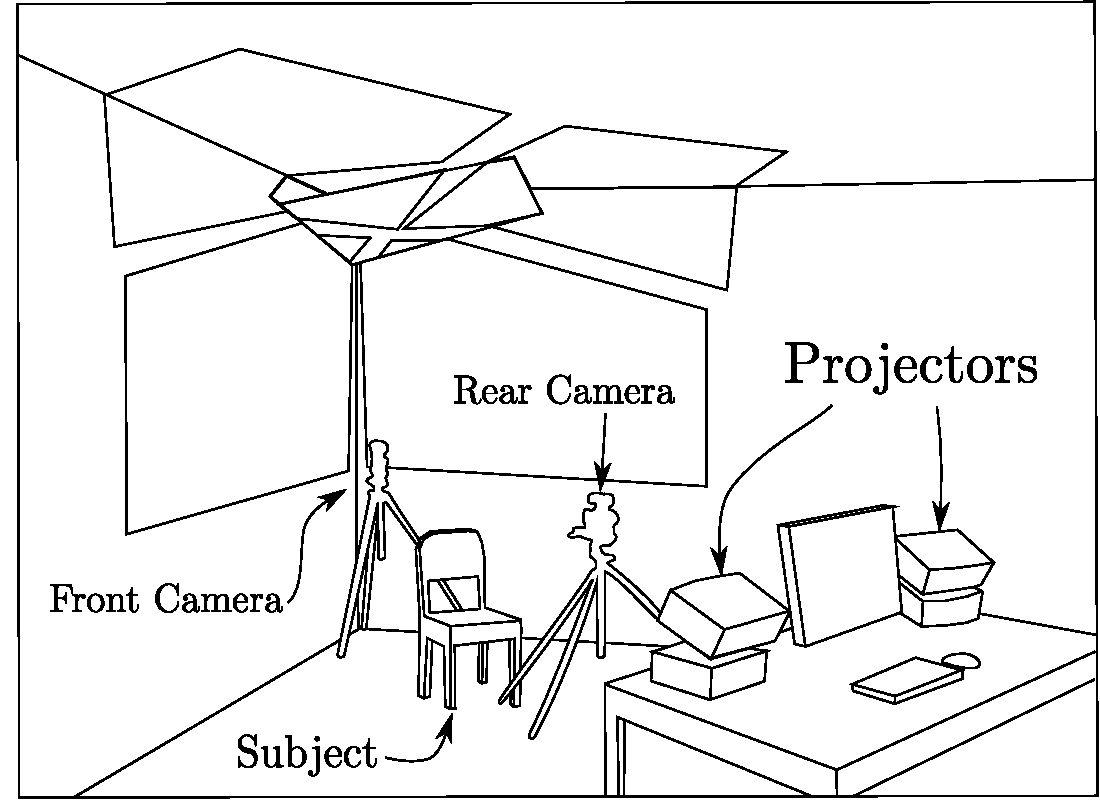
\includegraphics[height=2.5in]{figures_pami/camera_rig.pdf}
\caption{\small{\bf Training acquisition system:} Four projectors and two cameras controlled by one computer.}
\label{fig:system}
\end{figure}
With our projector system, our choice of illuminations is
constrained only by the need to achieve a good
SNR,\footnote{Since illuminations with more pixels illuminated
will have a better SNR (provided they don't saturate), there is
an engineering tradeoff between the SNR and the number of
training images.} avoid saturation, and achieve a reasonably
short acquisition time.  Two simplifying assumptions that we
make are that every pixel is either turned fully on or off in
every illumination, and that the illuminated regions do not
overlap.

Assuming that each pixel is fully on or off enables us to guarantee
that each illumination image has the same overall intensity, merely
by guaranteeing that we illuminate the same number of pixels in each image.\footnote{Since DLP projectors may have dramatically different response
curves depending on the mode they are in, it is not advisable to simply normalize each illumination image by its mean.}
Since our algorithm depends only on  the
linearity between the illuminations and the images, and not on the
relative intensities of the illuminations, the designer has the freedom to choose the overall intensity of the illuminations
to prevent saturation or low SNR, in a sort of offline exposure control.

Assuming that the sequentially illuminated regions do not overlap results in a
set of training images that span a larger cone than a similar number of
overlapping regions.  This results in training images that require fewer
negative coefficients in $\x$ to represent test images under natural
illuminations.  The effect of negative coefficients in $\x$ appears to depend
partly on how the test images are taken and is still under study.

{\em Relationship to existing work:} Most light stages used for face recognition have
been constructed for the purpose of creating public data sets to study
illumination invariance \cite{Georghiades2001-PAMI, Gross2008-FGR}.  Many other
light stages have been used for computer graphics purposes
\cite{debevec2000acquiring, jones2005performance}.
The light source can be
moved around manually \cite{masselus2002free}, but this may result in poor
consistency of illuminations between users.  Structured light applications use projectors to
directly illuminate the face (or other object) \cite{zhang2002rapid} for 3D
reconstruction, but this is very disturbing to the user.
Y.\ Schechner \cite{schechner2007multiplexing}
studies techniques for multiplexing illumination that can dramatically reduce the noise
of the demultiplexed images for certain classes of objects and cameras.
While these techniques have not been incorporated into the current
system, they fit elegantly into our framework and will likely be used
in future implementations.  We stress that use of this multiplexing technique
is independent from the choice of original (directional) illuminations.

\subsection{Choice of Illumination Patterns}

We ran two experiments to guide our choice of illuminations for
our large-scale experiments:
\begin{enumerate}
\item {\em Coverage Experiment.} In the first experiment we
    attempt to determine what coverage of the sphere is
    required to achieve good interpolation for test images.
    The subject was illuminated by 100 (50 front, 50 back)
    illuminations arranged in concentric rings centered at
    the front camera.  Subsets of the training images were
    chosen, starting at the front camera and adding a ring
    at a time.  Each time a ring was added to the training
    illumination set, the average $\ell^1$ registration
    error (residual) for a set of test images taken under
    sunlight was computed and plotted in Figure
    \ref{fig:illumination-patterns}(a).  The more rings of
    training illuminations are added, the lower the
    representation error becomes, with diminishing returns.
\item {\em Granularity Experiment.} In the second
    experiment we attempt to determine how finely divided
    the illumination sphere should be.  At the first
    granularity level, the projectors  illuminate the
    covered area uniformly.  At each subsequent granularity
    level each illuminated cell is divided in two along its
    longer side but intensity doubled.  For each
    granularity level the average $\ell^1$ registration
    error is computed as in the coverage experiment and
    shown in Figure \ref{fig:illumination-sufficiency}(b).
    Again, diminishing returns are observed as more
    illuminations are added.
\end{enumerate}
\begin{figure}
\centering
\begin{tabular}{cc}
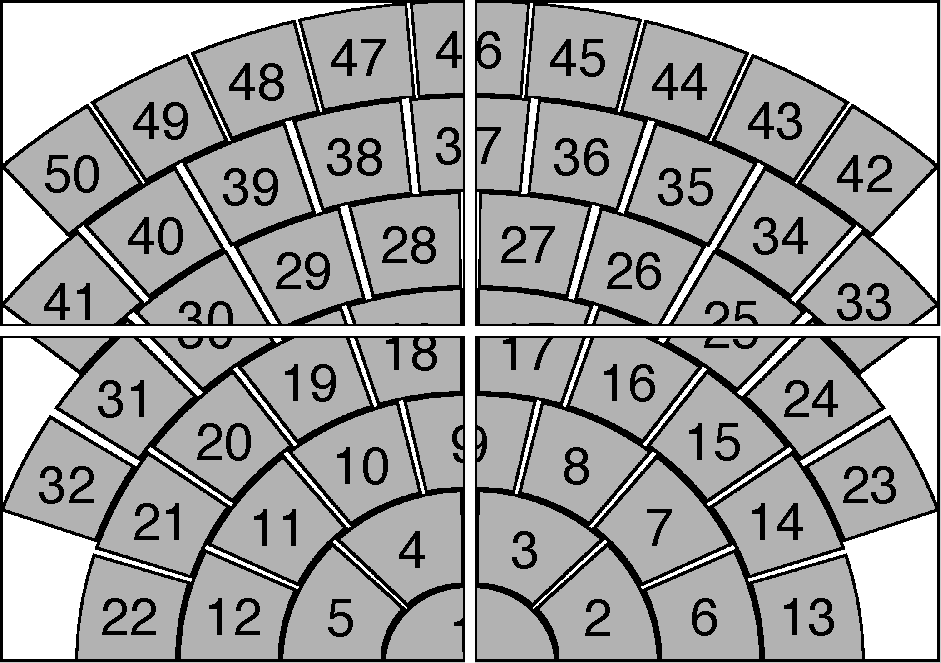
\includegraphics[height=1.7in]{figures_pami/coverage_experiment_asplode.png} &
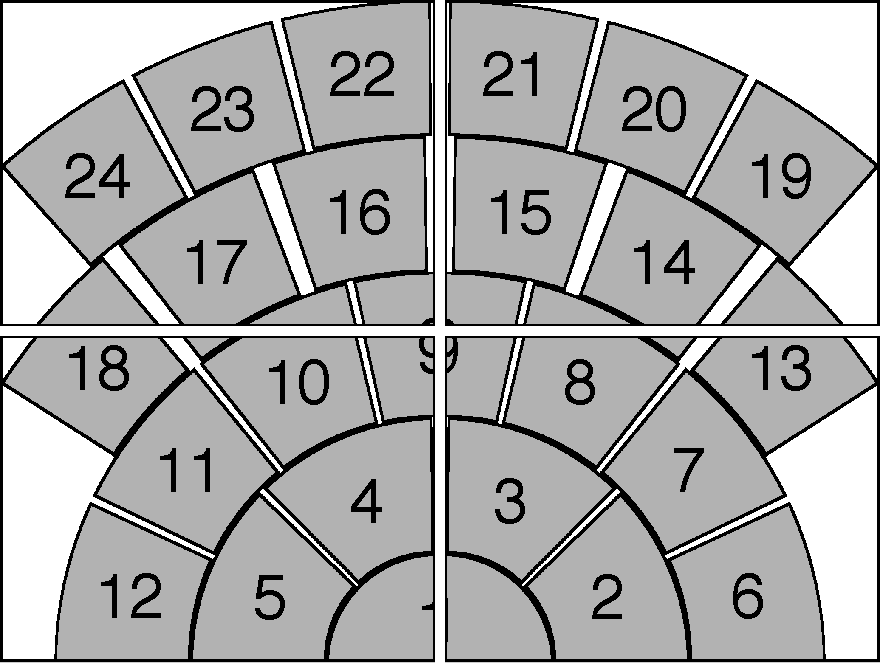
\includegraphics[height=1.7in]{figures_pami/final_cvpr_illuminations_asplode.png}  \\
(a) Coverage Experiment & (b) Chosen Illumination Patterns
\end{tabular}
\caption{\small{\bf Illumination Patterns.}   The cells are illuminated in sequence.  For rear illuminations the sequence is reversed.  In the chosen pattern's rear illumination, the cells 1-5 and 7-11 are omitted for a total of 38 illuminations. The four rectangular regions correspond to the four projectors.  }
\label{fig:illumination-patterns}
\end{figure}

\begin{figure}
\centering
\begin{tabular}{@{}c@{}c@{}}
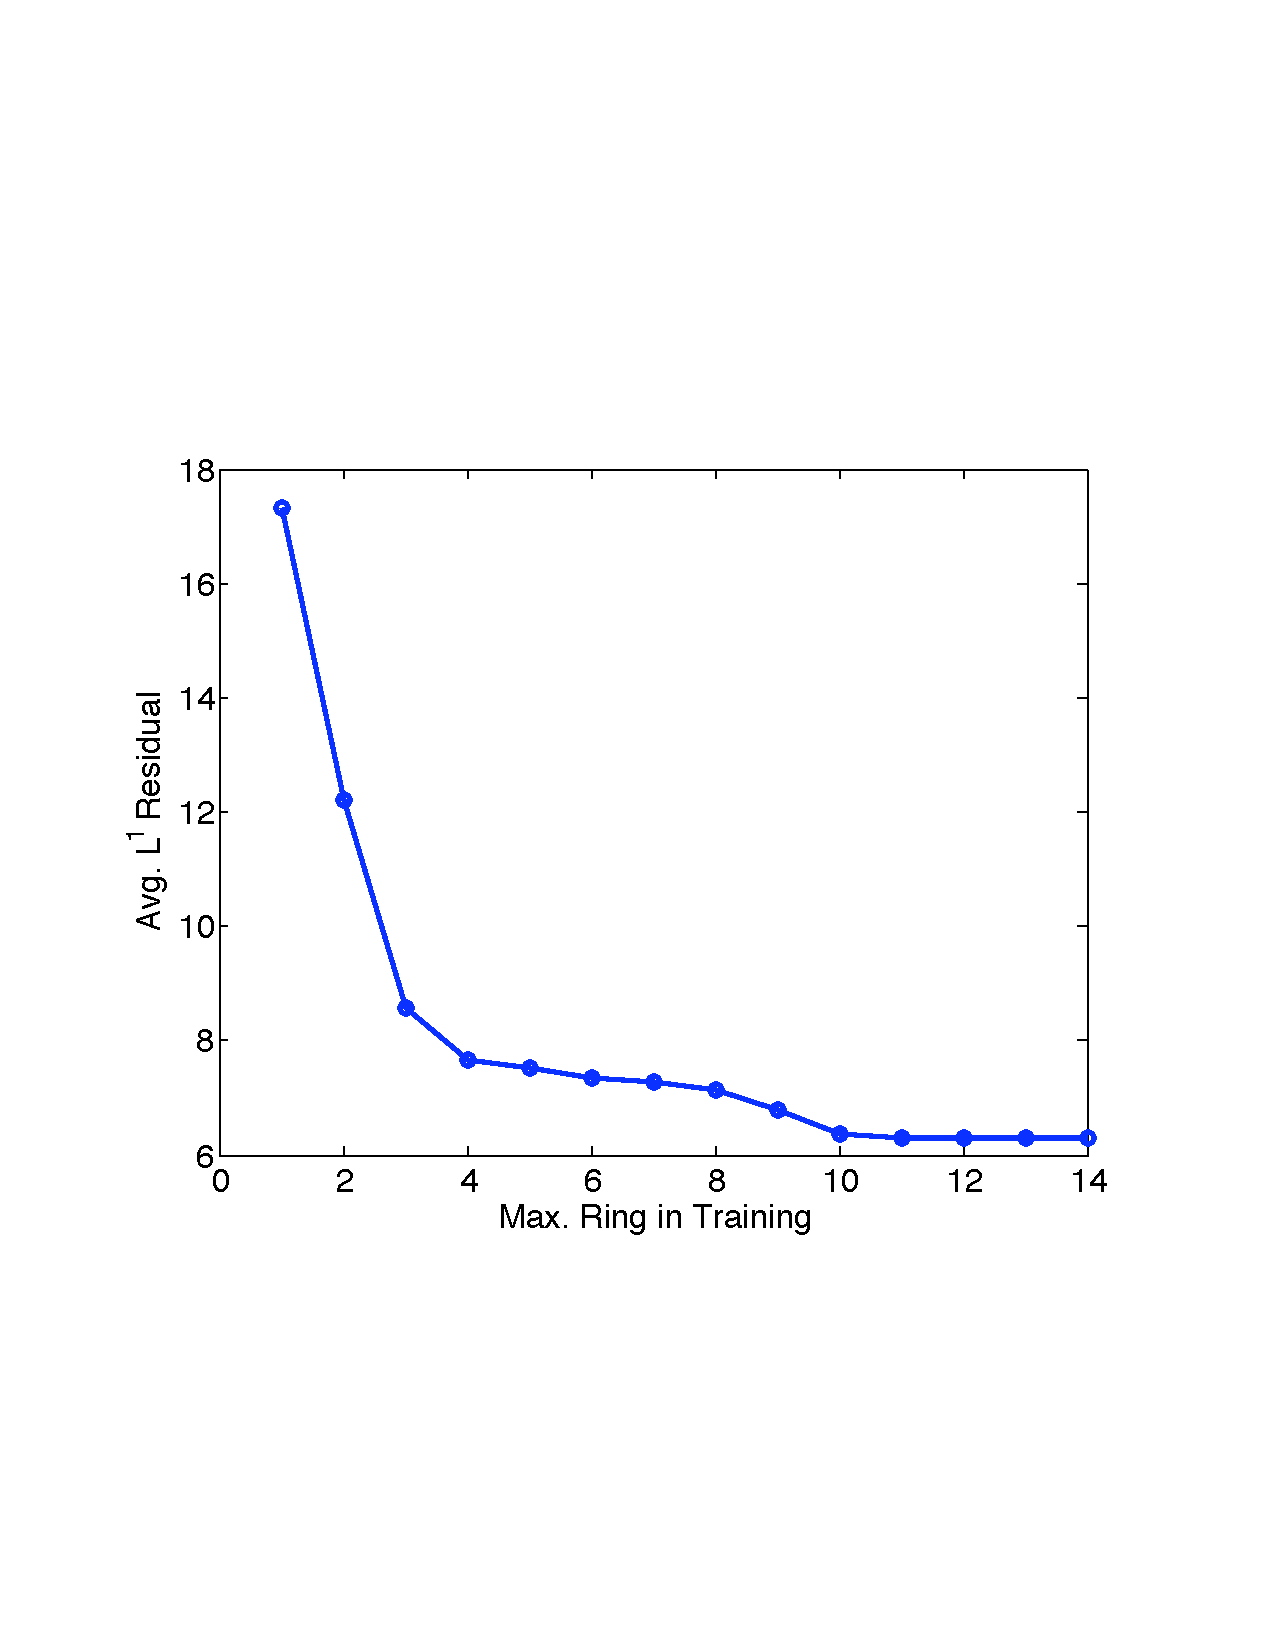
\includegraphics[height=2in]{figures_pami/illum_results/coverage_sunset.pdf} &
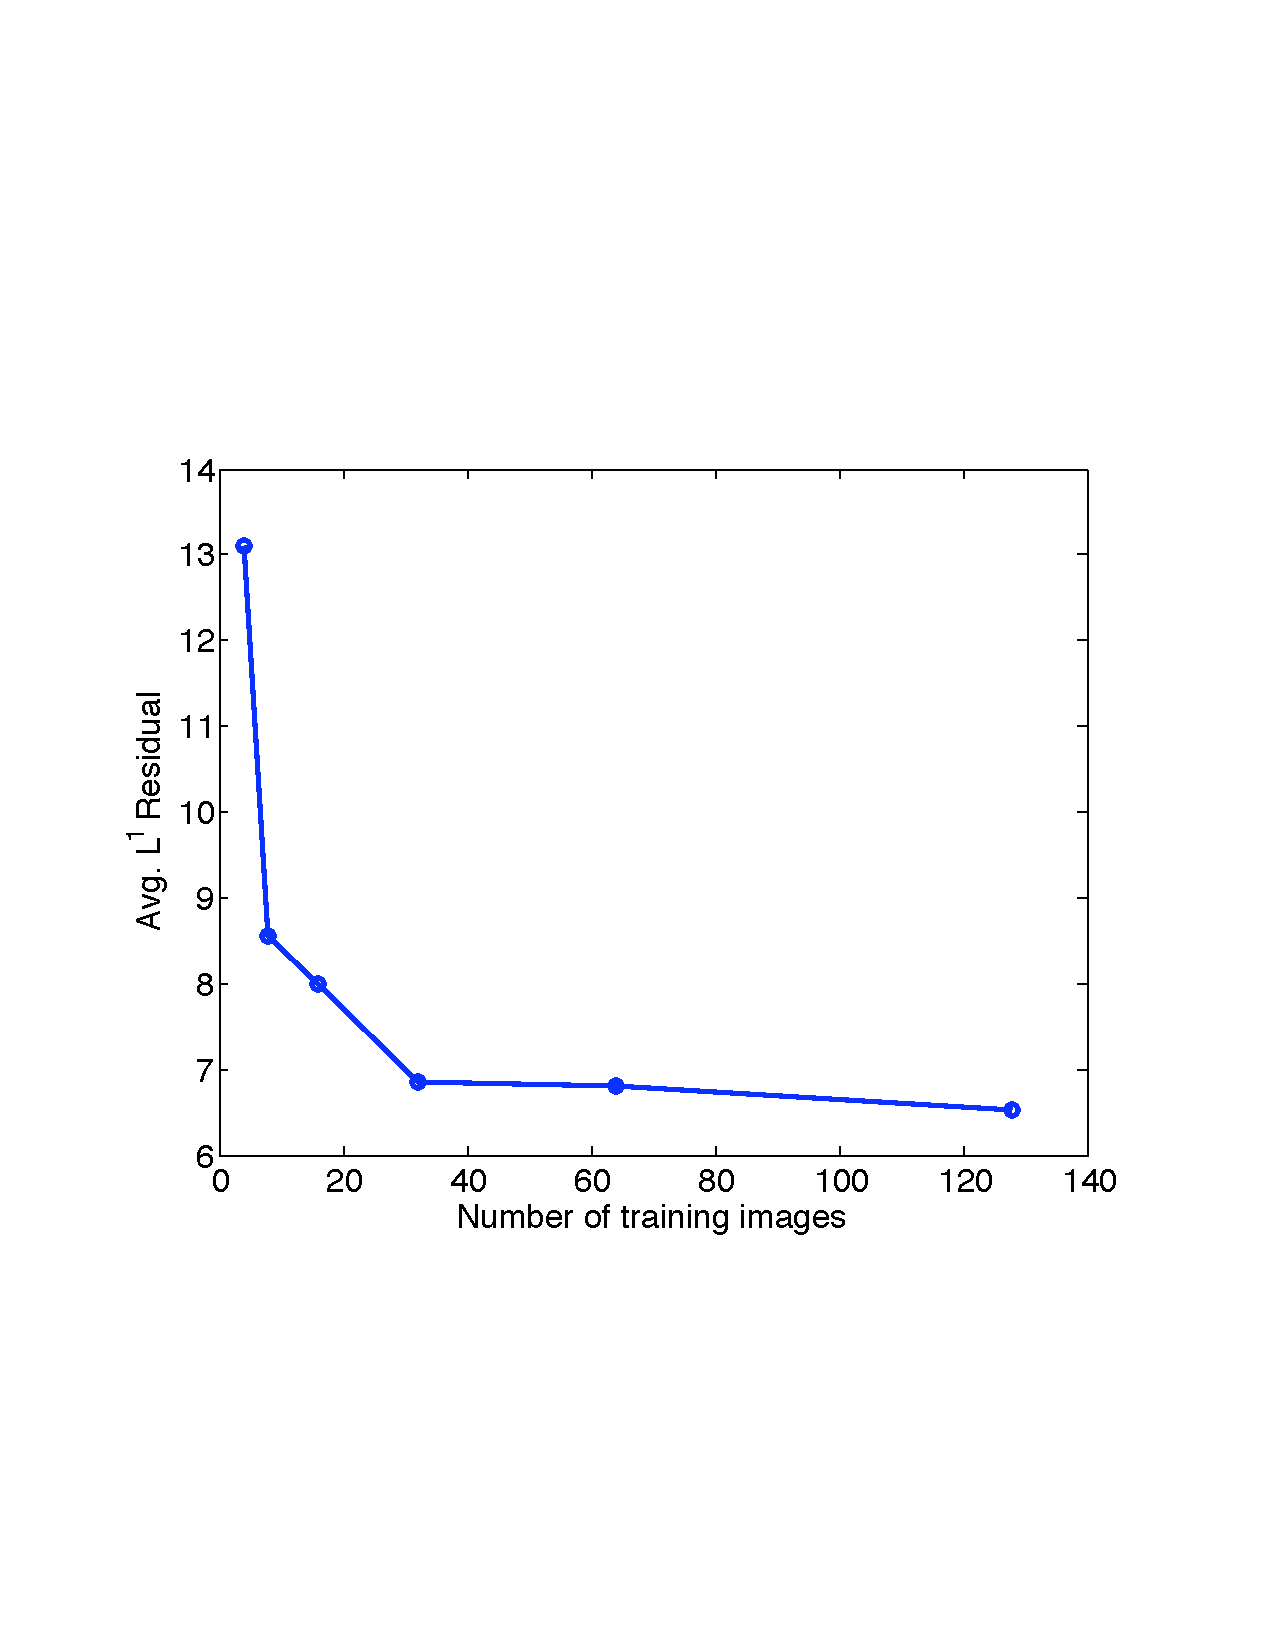
\includegraphics[height=2in]{figures_pami/illum_results/granularity_sunset.pdf} \\
(a) Coverage & (b) Granularity
\end{tabular}
\caption{\small{\bf Study of sufficient illuminations.} The average $\ell^1$ registration residual versus different illumination training sets. }
\label{fig:illumination-sufficiency}
\end{figure}

In the plot for the coverage experiment, Figure
\ref{fig:illumination-sufficiency}(a),
 we clearly see two plateau regions: one is after 4 rings
and one is after 10 rings. The first four rings represent the
typical frontal illuminations, which are present in most public
face datasets; however, we see that the residual stabilizes
after 10 rings which include some illuminations from the back
of the subject. This suggests that although the frontal
illuminations account for most of the illumination on the face,
some illuminations from the back are needed in the training set to
represent images with illumination coming from all directions.
In the plot for the granularity experiment, Figure
\ref{fig:illumination-sufficiency}(b), we observe that the
residual reaches a plateau after four divisions, corresponding
to a total of 32 illuminations. Based on the results from both
experiments, we decide to partition the area covered by the
first 10 rings into a total of 38 cells, whose layout is
explained in Figure \ref{fig:illumination-patterns}(b). For
our large-scale experiments, we have collected those
illuminations for all our subjects.\footnote{It is possible
that with further experimentation a reduced set of illuminations
can be found that performs as well or better.}

See below for the 38 training images of one subject:
\begin{figure}[h]
\centering
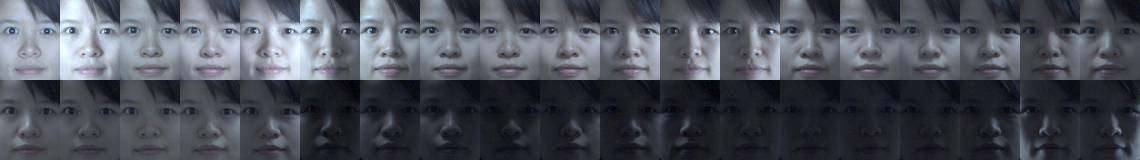
\includegraphics[width=\textwidth]{figures_pami/training.png}
\end{figure}


%\subsection{Should Positivity in the Representation Coefficients
%be Enforced?} One critical issue in linear illumination models
%is whether to enforce nonnegativity in the coefficients $\x$,
%i.e. whether to model illumination using a cone or a subspace.
%Some authors, i.e. \cite{Basri2003-PAMI}, have chosen to allow
%negative components in the coefficient vector $\x$ when
%representing one image as a sum of other images, and only
%enforce that the linear combination $A\x$ be positive
%everywhere.  Unfortunately, for non-convex objects such as
%faces, enforcing non-negativity of the representation is not
%sufficient to guarantee that the resulting image of the object
%is physical.  For example, consider a Lambertian planar object
%with a cylindrical hole drilled in it that is aligned with the
%optical axis of an orthographic camera.  Consider two images:
%one under illumination from a distant point source aligned with
%the hole, and one off of the hole axis.  Positively weighting
%the on-axis image and negatively weighting the on-axis image
%can result in an image where the bottom of the hole is more
%strongly illuminated than the surrounding plane.  The image is
%positive, but it is clearly non-physical.  It is worth
%emphasizing that this phenomenon is a result of some points on
%an object seeing a restricted subset of the illumination sphere
%(a violation of convexity),  and not a result of the
%directionality of the light chosen in the thought experiment.
%While the number of coefficients that actually end up negative
%after optimization is usually very small, we have observed
%pathological cases where the shadows next to the user's nose in
%the reconstructed image invert in value.

%Instead of using a smaller set of training images, allowing the
%coefficients to go negative to try to represent more test
%illuminations, and risking over-fitting, we decided to enforce
%non-negativity of the coefficients.  Nonnegative combinations
%of images are guaranteed to correspond to physically plausible
%images.  all physical illuminations unless the training images
%actually span the boundary of the illumination cone. Because we
%have a flexible acquisition system, we can directly generate a
%set of illuminations that span most of the illumination cone,
%without resorting to negative coefficients and risking
%overfitting.  Thus, in Algorithm 1, we have enforced that the
%coefficients $\x$ be non-negative.

%One of the main factors that complicates face recognition, and computer vision in general, is that two images of the same person's face can be very different, even if the pose is carefully controlled and all points on the person's face are visible in both images.  The most safe, reliable, and general assumption that can be made about the imaging process is that it is linear with respect to the intensity of different light sources.  The set of images of a given object is therefore a cone in the non-negative orthant of the pixel basis.  All recognition algorithms that rely on vision for training rely on images sampled from this cone.


\section{Tests on Public Databases}\label{sec:multipie}
In this section and the next section, we conduct comprehensive experiments on
large-scale face databases to verify the performance of our algorithm and
system. We first test on the largest public face database available that is
suitable for testing our algorithm, the CMU Multi-PIE.  One shortcoming of the
CMU Multi-PIE database for our purposes is that there is no separate set of
test images taken under natural illuminations; we are left to choose which sets
of images to use for testing and training.  To challenge our algorithm, we
choose only a small set of illuminations for the training set, yet we include
all illuminations in the testing set. In the following section, we will test
our algorithm on a face dataset that is collected by our own system. The goal
for that experiment will be to show that with a sufficient set of training
illuminations for each subject, our algorithm indeed works stably and robustly
with practical illumination, misalignment, pose, and occlusion, as already
indicated by our experiment shown in Figure \ref{fig:promo}(bottom).

CMU Multi-PIE provides the most extensive test set among public
datasets. This database contains images of 337 subjects across
simultaneous variation in pose, expression, and illumination.
Of these 337 subjects, we use all of the 249 subjects present
in Session 1 as the training set. The remaining 88 subjects are
treated as ``impostors'', or invalid images. For each of the
249 training subjects, we include frontal images of 7 frontal
illuminations,\footnote{They are illuminations
$\{0,1,7,13,14,16,18\}$ of \cite{Gross2008-FGR}. For each
directional illumination, we subtract the ambient-illuminated
image 0.} taken with neutral expression. As suggested by the
work of \cite{Georghiades2001-PAMI}, we choose these extreme
frontal illuminations in the hope that they would linearly
represent other frontal illuminations well. For the test set,
we use all 20 illuminations from Sessions 2-4, which were
recorded over a period of several months. The dataset is
challenging due to the large number of subjects, and due to
natural variation in subject appearance over time.
Table \ref{tab:MultiPIE-recognition2} shows the result of our
algorithm on each of the 3 testing sessions. Our algorithm
achieves recognition rates above $90\%$ for all three sessions.
For the test images, our iterative alignment was initialized
automatically via the Viola and Jones' face detector. To
demonstrate that the sparse representation based recognition
step is indeed beneficial even when there are no impostors, we
include results for recognition based only on the alignment
error residuals (i.e. $S=1$), shown in row 1.

\begin{table}
\caption{Recognition rates on the Multi-PIE database for
Algorithm 1 and \cite{Yang2010-CVPR}}
\centerline{
\begin{tabular}{|c|c|c|c|c| }
\hline
Recognition rate & Session 2 & Session 3 & Session 4  \\
\hline
{Alg. 1, $S=1$} & 90.7\% & 89.6\% & 87.5\% \\
\hline
{Alg. 1} & 93.9\% & 93.8\% & 92.3\% \\
\hline
{Alg. 1 with improved window} & 95.0\% & {\bf 96.3}\% & {\bf 97.3}\% \\
\hline
\cite{Yang2010-CVPR} & {\bf 95.2}\% & 93.4\% & 95.1\% \\
\hline
\end{tabular}
\label{tab:MultiPIE-recognition2} }
\end{table}

\newcommand{\tempwidth}[0]{0.9in}
\begin{figure}
\centering
{
\begin{tabular}{@{}c@{}c@{}c@{}c@{}c@{}c@{}}
\hspace{-2mm}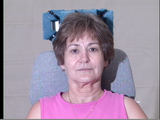
\includegraphics[width=\tempwidth,clip=true]{figures_pami/multipie_failed/079_01_01_051_08.png}  &
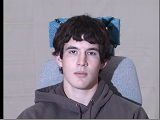
\includegraphics[width=\tempwidth,clip=true]{figures_pami/multipie_failed/111_01_01_051_08.png}  &
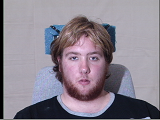
\includegraphics[width=\tempwidth,clip=true]{figures_pami/multipie_failed/196_01_01_051_08.png}  &
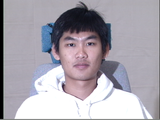
\includegraphics[width=\tempwidth,clip=true]{figures_pami/multipie_failed/130_01_01_051_08.png}  &
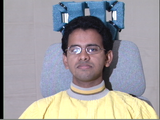
\includegraphics[width=\tempwidth,clip=true]{figures_pami/multipie_failed/163_01_01_051_08.png}  &
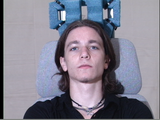
\includegraphics[width=\tempwidth,clip=true]{figures_pami/multipie_failed/175_01_01_051_08.png} \\
\hspace{-2mm}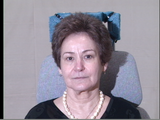
\includegraphics[width=\tempwidth,clip=true]{figures_pami/multipie_failed/079_02_01_051_08.png}  &
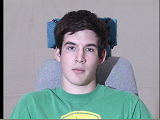
\includegraphics[width=\tempwidth,clip=true]{figures_pami/multipie_failed/111_02_01_051_08.png}  &
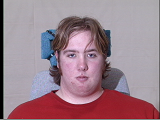
\includegraphics[width=\tempwidth,clip=true]{figures_pami/multipie_failed/196_02_01_051_08.png}  &
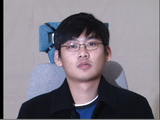
\includegraphics[width=\tempwidth,clip=true]{figures_pami/multipie_failed/130_02_01_051_08.png}  &
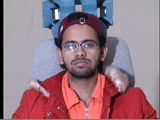
\includegraphics[width=\tempwidth,clip=true]{figures_pami/multipie_failed/163_02_01_051_08.png}  &
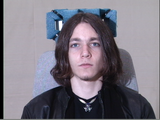
\includegraphics[width=\tempwidth,clip=true]{figures_pami/multipie_failed/175_02_01_051_08.png} \\
\hspace{-2mm}(a) & (b) & (c) & (d) & (e) & (f) 
\end{tabular}
}
\caption{\small{\bf Representative failures from Multi-PIE}. {\bf Top:} training from Session 1; {\bf Bottom:} test images from Session 2. Due to changes in hair, glasses, beard, or pose, our alignment fails on these subjects regardless of test image illumination.}
\label{fig:failed-examples}
\end{figure}
\subsection{Improving the Sampling Window}
Our algorithm's errors are mostly caused by a few subjects who
significantly change their appearances between sessions (such
as hair, facial hair, and eyeglasses). Some representative
examples are shown in Figure \ref{fig:failed-examples}. For those subjects, alignment and recognition fail on
almost all test illuminations.
\begin{figure}[b]
\centering
{
\begin{tabular}{@{}cc@{}}
\includegraphics[trim=1.9in .7in 1.9in .5in, clip, height=1.8in]{figures_pami/example.png} &
\includegraphics[trim=1.9in .7in 1.9in .5in, clip, height=1.8in]{figures_pami/example_new.png} \\
Default window. & Proposed window.
\end{tabular}
}
\caption{\small{\bf Choosing different sampling windows.}}
\label{fig:new-mask}
\end{figure}
Meanwhile, this observation also suggests that we might be able
to improve the performance of our method by carefully choosing
a face region which is less affected by the above factors for
recognition. In particular, since the forehead region is likely
to be affected by the change of hair style, we try replacing
the previous $80 \times 60$ canonical frame with a new
window that better excludes the forehead. We adjust the
resolution of the window to keep $m$ approximately constant. In addition,
we cut off two lower corners of the $80 \times 60$ canonical frame, motivated by
the observation that in many cases the corners
actually contain background. An example of the new window
is shown in Figure~\ref{fig:new-mask}.

\begin{table*}
\centering
\small
\caption{\small Recognition rates on the Multi-PIE database for
different pairings of alignment and recognition stages.}
\centerline{
\begin{tabular}{|c|c|c|c|c|c|c|c|c|c|c| }
\hline
\backslashbox{Rec.}{Align.}
& \multicolumn{3}{|c|}{Face Detector}
& \multicolumn{3}{|c|}{Manual}
& \multicolumn{3}{|c|}{Iterative Alignment}
\\
\hline
Session $\rightarrow$	& 2		&3			&4			& 2		&3			&4			& 2		&3			&4		\\
\hline
NS	& 30.8\%	& 29.4\%	& 24.6\%	& 77.6\%	& 74.3\%	& 73.4\%	& 84.5\%	& 82.3\%	& 81.4\% \\
\hline
NN	& 26.4\%	& 24.7\%	& 21.9\%	& 67.3\%	& 66.2\%	& 62.8\%	& 73.5\%	& 69.6\%	& 69.3\% \\
\hline
LDA	& 5.1\%		& 5.9\%		& 4.3\%		& 49.4\%	& 44.3\%	& 47.9\%	& 91.0\%	& 89.9\%	& 88.1\% \\
\hline
LBP	& 39.9\%	& 38.1\%	& 33.9\%	& 93.3\%	& 91.2\%	& 92.9\%	& {\bf 95.2\%}	& {\bf 94.7\%}	& {\bf 93.5\%} \\
\hline
SRC	& -- & -- & -- & -- & -- & -- & 93.9\%	& 93.8\%	& 92.3\% \\
\hline
\end{tabular}
\label{tab:MultiPIE-recognition} }
\end{table*}

Table \ref{tab:MultiPIE-recognition2} shows that the
recognition rates on Multi-PIE indeed increase with this new
window. In addition, Figure \ref{fig:failed-examples}(a), (b),
and (c) illustrate three representative subjects for which the
recognition rates of our algorithm are significantly boosted
with the new window. However, we should mention that the best
choice of the window is problem-specific and there is not a
simple guideline to follow. For example, although the new
window performs better on Multi-PIE, the same window does not
help at all on our own database, which will be introduced in
the next section. This is because most of the training and
testing images in our database are taken on the same day so the
variation in hair style is very small. Hence, excluding the
forehead part may actually result in loss of useful
discriminative information.

\subsection{Comparison to Existing Work}

We first compare our result to the recent work
\cite{Yang2010-CVPR}. Notice that in \cite{Yang2010-CVPR}, the
initial registration is obtained from manually selected outer
eye corners. Then, a supervised hierarchical sparse coding
model based on local image descriptors is trained, which enjoys
certain translation invariant properties. With the same
training and testing sets, \cite{Yang2010-CVPR} is able to
handle the remaining misalignment and achieves state-of-the-art
performance on the CMU Multi-PIE database.
Table~\ref{tab:MultiPIE-recognition2} shows that our algorithm
achieves similar or better performance on different sessions of
Multi-PIE.

% Classical algorithms
To better examine the effectiveness of our iterative alignment
algorithm, we next compare our result to baseline
linear-projection-based algorithms, such as Nearest Neighbor
(NN), Nearest Subspace (NS) \cite{Lee2005-PAMI}, and Linear
Discriminant Analysis (LDA)
\cite{Belhumeur1997-PAMI}.\footnote{We do not list results on
PCA \cite{Turk1991-CVPR} as its performance is always below
that of Nearest Subspace.} Since these algorithms assume
pixel-accurate alignment, they are not expected to work well if
the test image is not well aligned with the training. In
Table~\ref{tab:MultiPIE-recognition}, we report the results of
these classical algorithms with three types of testing image
alignment: 1.\ alignment from the Viola and Jones' detector,
2.\ alignment via manually selected outer eye
corners,\footnote{Two manually clicked points are sufficient to
define a similarity transformation. All of the experiments in
this section are carried out with similarity transformations.}
and 3.\ the output of our iterative alignment algorithm. The
performance drop of the LDA algorithm on Multi-PIE reported
here seems to agree with that reported already in
\cite{Gross2008-FGR}.  All of the classical algorithms benefit
greatly from being paired with our iterative alignment
algorithm.

% LBP
We also compare our result to Local Binary Patterns (LBP)
\cite{Ahonen2006-PAMI}, a local appearance descriptor which is
able to capture fine details of facial appearance and texture.
Due to its robustness to variations in illumination, facial
expression, aging and other changes, LBP has achieved the
state-of-the-art face recognition performance in the scenario
when only one sample per person is used for training
\cite{Tan06facerecognition}. In this section, we follow the same
steps as in \cite{Ahonen2006-PAMI} to construct an LBP
descriptor for each training and testing sample. The $80\times
60$ face region is first divided into a regular $10\times 10$
grid of cells, each of size $8\times 6$ pixels. Within each
cell, the histogram of 59 uniform binary patterns is then
computed, where the patterns are generated by thresholding 8
neighboring pixels in a circle of radius 2 using the central
pixel value. Finally, the local histograms are concatenated to
produce the global descriptor vector. As suggested in
\cite{Ahonen2006-PAMI}, the recognition is performed using a
nearest neighbor classifier with Chi square distance as the
distance measure and we report the recognition rates with the
same three types of input as before.

As shown in Table~\ref{tab:MultiPIE-recognition}, although LBP
achieves competitive recognition rates given manually aligned
training and testing samples, demonstrating its robustness to
moderate misalignment, it still benefits from using the output
of our iterative alignment algorithm as the input. In addition,
like the other classical algorithms, the performance of LBP
degrades dramatically if it is applied directly to the output
of a face detector. This is notable given that LBP is often
applied without any special alignment in practice. Finally, we
attribute the improvement in performance of LBP over SRC in
this experiment to its robustness to illumination components
that cannot be linearly interpolated by the training set.

In addition, although our algorithm is not designed for
recognition when there is only a single gallery image per user,
we compare its performance with LBP within this setting for
completeness. For this experiment, we use the FERET dataset
\cite{phillips1998feret}, which contains five standard
partitions: `fa' is the gallery containing 1196 frontal images
of 1196 subjects, and `fb', `fc', `dup1' and `dup2' are four
sets of probe images. The testing sets differ from the training
in facial expression (`fb'), illumination (`fc'), aging (`dup1'
) and long aging (`dup2'). In fact, except for `fb', we notice
significant changes of illumination in all the other three test
sets. For the training, we again crop and normalize the face
region from each original image to an $80\times 60$ window
using manually marked eye coordinates \cite{Deng2010-PR}. In
Table~\ref{tab:FERET-recognition}, we report the performance of
our algorithm on the four test sets, with input directly
obtained from the Viola and Jones' detector. We also report the
performance of LBP with the same three types of input as before:
we use letters
``$d$'', ``$m$'', and ``$i$'' to indicate face detector, manual
alignment, and our iterative alignment algorithm, respectively.

As expected, our algorithm does not perform well except for
`fb', in which the illumination is similar to the training and
the mere variation in facial expression is handled well by the
sparse error model. For the other three test sets, our
algorithm fails because the illumination changes and other
variations seriously violate the assumptions of our method.
This also explains why LBP performs worse with our iterative
alignment algorithm, compared to manual alignment. On the other
hand, while LBP achieves the best recognition rates given
manually aligned training and testing samples, its performance
degrades drastically when the input is obtained directly from
the face detector. It is also worth noting that similar poor
performance of LBP, as well as other descriptors, has been
observed on the Labeled Face in the Wild (LFW) database, where
the training is uncontrolled and limited and the input is
directly obtained from the face detector \cite{Wolf2008-ECCV}.
\begin{table}
\caption{Performance on single gallery image FERET dataset}
\centerline{
\begin{tabular}{|c|c|c|c|c| }
\hline
Recognition rate \% & fb & fc & dup1 & dup2 \\
\hline
$LBP_d$ & 54.8 & 10.3 & 29.8 & 19.8 \\
\hline
$LBP_m$ & {\bf 96.6} & {\bf 58.8} & {\bf 71.6} & {\bf 61.5} \\
\hline
$LBP_i$ & 94.5 & 42.8 & 46.5 & 21.1 \\
\hline
{Alg. 1} & 95.2 & 28.4 & 46.1 & 20.3 \\
\hline
\end{tabular}
\label{tab:FERET-recognition} }
\end{table}

All of these experimental results confirm that
both illumination and alignment need to be simultaneously handled
well in order to achieve accurate face recognition, even when there is
no obvious occlusion or corruption in the test.

\subsection{Subject Validation}

We test the algorithms' ability to reject invalid images of the
88 subjects not appearing in the training database. As
mentioned before, the \emph{sparsity concentration index} (SCI)
is used as the outlier rejection rule. Given the sparse
representation $\x$ of a test image with respect to $K$
training classes, the SCI measures how concentrated the
coefficients are on a single class in the dataset and is
defined as in \cite{Wright2009-PAMI}:
\begin{displaymath}
\textup{SCI}(\x) \doteq \frac{K \cdot \max_i \|\delta_i(\x)\|_1 /
\|\x\|_1 - 1}{K - 1} \in [0,1] .
\end{displaymath}
It is easy to see that if $\textup{SCI}(\x) = 1$, the test
image is represented using images from one single subject
class; if $\textup{SCI}(\x) = 0$, the coefficients are spread
evenly over all classes. Thus, we can choose a threshold $t \in
[0,1]$ for the proposed method and accept a test image as valid
if $\textup{SCI}(\x) \geq t$, and otherwise reject it as
invalid. We compare this classifier to classifiers based on
thresholding the error residuals of NN, NS, LDA, and LBP.
\begin{figure}[t]
{
\centerline{
\begin{tabular}{@{}cc@{}}
\includegraphics[height=2.5in]{figures_pami/pami_roc_revision2} &
\includegraphics[height=2.5in]{figures_pami/pami_roc2} \\
(a) & (b) \\
\end{tabular}
}}
\caption{\small {\bf ROC curves} for subject validation on Multi-PIE database,
(a) for all algorithms with iterative alignment, and
(b) for the classical algorithms with manual alignment (indicated by a subscript ``m'').}\label{fig:roc-multipie}
\end{figure}

Figure \ref{fig:roc-multipie} plots the receiver operating
characteristic (ROC) curves, which are generated by sweeping
the threshold $t$ through the entire range of possible values
for each algorithm.\footnote{Rejecting invalid images not in
the entire database is much more difficult than deciding if two
face images are the same subject. Figure \ref{fig:roc-multipie}
should not be confused with typical ROC curves for face
similarity, e.g., \cite{PhillipsP2007}.} On the left we can see
that the SCI based recognition approach significantly
outperforms the other algorithms, including LBP, even when all
algorithms are coupled with our proposed iterative alignment.
In the right plot we again see that classical algorithms, and
even LBP, are very sensitive to alignment.  Similar contrasts
between our algorithm and baseline algorithms were also
observed for SRC in \cite{Wright2009-PAMI}, though on much
smaller datasets.

\subsection{Recognition with Synthetic Random Block Occlusion}

We further test the robustness of our $\ell^1$-norm based
algorithm to synthetic occlusion. We simulate various levels of
occlusion from 10\% to 50\% by replacing a randomly located
block of the face image with an image of a baboon, as shown in
Figure~\ref{fig:multipie-occ-rec}. In this experiment, to avoid
any other factors that may contribute to extra occlusion of the
face (such as the change of hair style), we choose illumination
10 from Session 1\footnote{This is the same session as the
training set.} as testing. The rest of the experimental setting
remains unchanged. The table in
Figure~\ref{fig:multipie-occ-rec} shows that our algorithm is
indeed capable of handling a moderate amount of occlusion. For
example, at 20\% occlusion, our algorithm still achieves 94.9\%
recognition rate.

\renewcommand{\tempwidth}{0.2\textwidth}
\begin{figure}
\centering
\begin{tabular}{@{}c@{}c@{}c@{}c@{}c@{}}
\includegraphics[width=\tempwidth,clip=true]{figures_pami/multipie_occ/occ10.png} &
\includegraphics[width=\tempwidth,clip=true]{figures_pami/multipie_occ/occ20.png} &
\includegraphics[width=\tempwidth,clip=true]{figures_pami/multipie_occ/occ30.png} &
\includegraphics[width=\tempwidth,clip=true]{figures_pami/multipie_occ/occ40.png} &
\includegraphics[width=\tempwidth,clip=true]{figures_pami/multipie_occ/occ50.png}  \\
\end{tabular}
\caption{\small{\bf Recognition under varying level of
random block occlusion.} The above row of images shows examples of occluded test images with occlusion level from 10\% to 50\%. Our method maintains high recognition rates up to 30\% occlusion:}
{
\begin{tabular}{|c|c|c|c|c|c| }
\hline
Percent occluded & 10\% & 20\% & 30\% & 40\% & 50\%  \\
\hline
Recognition rate & 99.6\% & 94.9\% & 79.6\% & 46.5\% & 19.8\% \\
\hline
\end{tabular}
}
\label{fig:multipie-occ-rec}
\end{figure}

\subsection{Recognition with Pose and Expression} We now run tests of
our algorithm on a subset of the images from Multi-PIE with pose and expression variation in the test set, although we do not model these variations explicitly.
Using the same training set as above, we test our algorithm on
images in Session 2 with $15^\circ$ pose, for all 20
illuminations. As expected, the recognition rate drops to 78.0\%. We also test our
algorithm on images in Session 3 with smile, again for all 20
illuminations. The recognition rate is 64.8\%. Of course, it is reasonable to expect that
the performance of our method will be significantly improved if pose and expression data
are available in the training.


\section{Tests on Our Own Database}\label{sec:own-data} Using the training acquisition
system we described in Section \ref{sec:illumination}, and shown in Figure
\ref{fig:system}, we have collected the frontal view of 109
subjects {\em without eyeglasses} under 38 illuminations shown
in Figure \ref{fig:illumination-patterns}. For testing our
algorithm, we have also taken 935 images of these subjects with
a different camera under a variety of practical conditions.

\subsection{Necessity of Rear Illuminations} To see how
training illuminations affect the performance of our algorithm
in practice, we now compare how well a few frontal
illuminations can linearly represent: 1. other frontal illuminations
taken under the same laboratory conditions, and 2. typical
indoor and outdoor illuminations. To this end, we use the face
database acquired by our system and use 7 illuminations per
subject as training. The illuminations are chosen to be similar
to the 7 illuminations used in the previous experiment on
Multi-PIE.\footnote{We use the illuminations $\{6, 9, 12,
13, 18, 21, 22\}$ shown in Figure
\ref{fig:illumination-patterns}(b) to mimic the illuminations
 $\{0, 1, 6, 7, 13, 14, 18\}$ in Multi-PIE.} We then test
our algorithm on the remaining $24 - 7 = 17$ frontal
illuminations for all the subjects. The recognition rate is
$99.8\%$, nearly perfect. We also test our algorithm on 310
indoor images and 168 outdoor images of these subjects taken
under a variety of lighting conditions (category 1 and 2
specified below), similar to the one shown in Figure
\ref{fig:promo}, and the recognition rates for indoor and
outdoor images drop down to $94.2\%$ and $89.2\%$,
respectively. This is a strong indication that
frontal illuminations taken under laboratory conditions
are insufficient for representing test images under typical indoor and
outdoor illuminations.

\renewcommand{\tempwidth}{0.1667\textwidth}
\begin{figure}
\centering
\begin{tabular}{@{}c@{}c@{}c@{}c@{}c@{}c@{}}
\includegraphics[width=\tempwidth,clip=true]{figures_pami/uiuc_example/normal_indoor/DSC_1318.JPG} &
\includegraphics[width=\tempwidth,clip=true]{figures_pami/uiuc_example/normal_indoor/DSC_1521.JPG} &
\includegraphics[width=\tempwidth,clip=true]{figures_pami/uiuc_example/normal_indoor/DSC_1673.JPG} &
\includegraphics[width=\tempwidth,clip=true]{figures_pami/uiuc_example/normal_indoor/DSC_1732.JPG} &
\includegraphics[width=\tempwidth,clip=true]{figures_pami/uiuc_example/normal_indoor/DSC_1941.JPG} &
\includegraphics[width=\tempwidth,clip=true]{figures_pami/uiuc_example/normal_indoor/DSC_3766.JPG} \\
\includegraphics[width=\tempwidth,clip=true]{figures_pami/uiuc_example/normal_outdoor/DSC_1574.JPG} &
\includegraphics[width=\tempwidth,clip=true]{figures_pami/uiuc_example/normal_outdoor/DSC_1622.JPG} &
\includegraphics[width=\tempwidth,clip=true]{figures_pami/uiuc_example/normal_outdoor/DSC_1641.JPG} &
\includegraphics[width=\tempwidth,clip=true]{figures_pami/uiuc_example/normal_outdoor/DSC_3522.JPG} &
\includegraphics[width=\tempwidth,clip=true]{figures_pami/uiuc_example/normal_outdoor/DSC_3707.JPG} &
\includegraphics[width=\tempwidth,clip=true]{figures_pami/uiuc_example/normal_outdoor/DSC_3772.JPG} \\
\includegraphics[width=\tempwidth,clip=true]{figures_pami/uiuc_example/glasses/DSC_1397.JPG} &
\includegraphics[width=\tempwidth,clip=true]{figures_pami/uiuc_example/glasses/DSC_1532.JPG} &
\includegraphics[width=\tempwidth,clip=true]{figures_pami/uiuc_example/glasses/DSC_1556.JPG} &
\includegraphics[width=\tempwidth,clip=true]{figures_pami/uiuc_example/glasses/DSC_1585.JPG} &
\includegraphics[width=\tempwidth,clip=true]{figures_pami/uiuc_example/glasses/DSC_1688.JPG} &
\includegraphics[width=\tempwidth,clip=true]{figures_pami/uiuc_example/glasses/DSC_4035.JPG} \\
\end{tabular}
\caption{\small{\bf Representative examples of categories C1-C3}. One row for each category.}\label{fig:examples1-3}
\end{figure}

\begin{figure}[t]
\centering
\begin{tabular}{@{}c@{}c@{}c@{}c@{}c@{}c@{}}
\includegraphics[width=\tempwidth,clip=true]{figures_pami/uiuc_example/sunglasses/DSC_1565.JPG} &
\includegraphics[width=\tempwidth,clip=true]{figures_pami/uiuc_example/sunglasses/DSC_3656.JPG} &
\includegraphics[width=\tempwidth,clip=true]{figures_pami/uiuc_example/sunglasses/DSC_3827.JPG} &
\includegraphics[width=\tempwidth,clip=true]{figures_pami/uiuc_example/sunglasses/DSC_4090.JPG} &
\includegraphics[width=\tempwidth,clip=true]{figures_pami/uiuc_example/sunglasses/DSC_4106.JPG} &
\includegraphics[width=\tempwidth,clip=true]{figures_pami/uiuc_example/sunglasses/DSC_4126.JPG} \\
\includegraphics[width=\tempwidth,clip=true]{figures_pami/uiuc_example/sunglasses_failed/DSC_1611.JPG} &
\includegraphics[width=\tempwidth,clip=true]{figures_pami/uiuc_example/sunglasses_failed/DSC_3528.JPG} &
\includegraphics[width=\tempwidth,clip=true]{figures_pami/uiuc_example/sunglasses_failed/DSC_3744.JPG} &
\includegraphics[width=\tempwidth,clip=true]{figures_pami/uiuc_example/sunglasses_failed/DSC_3995.JPG} &
\includegraphics[width=\tempwidth,clip=true]{figures_pami/uiuc_example/sunglasses_failed/DSC_4030.JPG} &
\includegraphics[width=\tempwidth,clip=true]{figures_pami/uiuc_example/sunglasses_failed/DSC_4095.JPG} \\
\end{tabular}
 \caption{\small{\bf Representative examples of category C4}. Top row: successful examples with our method using overlapping blocks. Bottom row: failures with our method using overlapping blocks.}\label{fig:examples4}
\end{figure}

\subsection{Large-Scale Test with Sufficient Training
Illuminations} Now we use all 109 subjects and 38 illuminations
in the training and test on 935 images taken under a variety of
practical illuminations and conditions. We have manually partitioned the test images into four main
categories:
\begin{description}
\item[C1:] 310 \emph{indoor} images of 72 subjects without
    eyeglasses, frontal view
    (Fig.~\ref{fig:examples1-3}, row 1).
\item[C2:] 168 \emph{outdoor} images of 48 subjects without
    eyeglasses, frontal view
    (Fig.~\ref{fig:examples1-3}, row 2).
\item[C3:] 211 images of 32 subjects with \emph{eyeglasses}
    (Fig.~\ref{fig:examples1-3}, row 3).
\item[C4:] 246 images of 56 subjects with \emph{sunglasses}
    (Fig.~\ref{fig:examples4}).
\end{description}
We apply Viola and Jones' face detector on these images and
directly use the detected faces as the input to our algorithm.
Table~\ref{tab:UIUC-recognition} reports the performance of our
algorithm on each category.
Since our focus is on face
recognition, the errors do not include failures of the face
detector on some of the more challenging images.
As one can see, our algorithm achieves higher than 95\%
recognition rates on categories 1-3. Furthermore, using the
full set of 38 illuminations indeed improves the performance of
our system under practical illumination conditions compared to
only using a small subset of 7 illuminations. However, the
performance dramatically drops when the faces are occluded by
various types of sunglasses, which could cover up to 40\% of
the entire face. Given the previous experimental results on
synthetic random block occlusions, and given that the
illuminations are more challenging, the result is not
surprising. In the next subsection, we will show how additional
assumptions can be used to improve the recognition performance.
\begin{table}[h]
\centering \caption{Recognition rates on our own
database.}
\begin{tabular}{|c|c|c|c|c| }
\hline
Test Category & C1 & C2 & C3 & C4  \\
\hline
\hline
Recognition Rate & 98.4\% & 95.8\% & 95.1\% & 40.9\% \\
\hline
\end{tabular}
\label{tab:UIUC-recognition}
\end{table}

\subsection{Improving the Performance with Occlusion using Overlapping Blocks}
A traditional approach to improve the performance of face
recognition under severe occlusion is to use subregions instead
the entire face as a whole. This idea has been explored in many
earlier works; see \cite{Pentland1994-CVPR, Wright2009-PAMI}
for examples. Since in most real world cases the occlusion is contiguous, it is reasonable to argue that a minority of the
subregions are likely to be affected by the occlusion. In this
section, we adopt the same idea and partition the face into four
overlapping blocks to better handle sunglasses. This
scheme is illustrated in Figure~\ref{fig:occ-block}. Notice
that in this example three out of the four blocks are partially
or almost completely occluded. In our experiment, each block is
of size $90\times 48$ and covers about two-fifths of the entire
face. The testing and training sets are partitioned in the same
way. We then independently apply
Algorithm~\ref{alg:deformable-src} and compute a sparse
representation after registration for each block independently
with respect to the training set. The recognition
results for individual blocks are then aggregated by voting.

\begin{figure}
\centering
\includegraphics[width=4in]{figures_pami/occ_block.png}
\caption{\small{\bf Using overlapping blocks to tackle contiguous occlusion.} (a) The test image, occluded by sunglasses. (b) The four overlapping blocks. (c) The sparse representation is calculated after alignment for each block independently. The red lines correspond to his true identity. (d) The true identity is successfully recovered by voting based on the SCI scores.}
\label{fig:occ-block}
\end{figure}

In this experiment, we found that the using the \emph{sparsity
concentration index} (SCI) scores for voting achieves higher
recognition rate than the residual measure used in Algorithm~\ref{alg:deformable-src}, on
category 4 (sunglasses) of our database. The recognition rate
is increased to 78.3\%, compared to 40.9\% obtained without
this partition scheme. This is another evidence of the superior
ability of SCI on subject validation, since a heavily occluded
block can be regarded as an outlier for recognition and should
be rejected while voting.

However, we should point out that a major problem with this
approach is that occlusion cannot always be expected to fall within
 any fixed partition of the face image. Therefore, the
proposed scheme should only be viewed as an example which shows
that the performance under occlusion can be boosted by
leveraging local information of a face as well as global information. We
leave the investigation of more general models (e.g., MRF \cite{ZhouZ2009}) for face
recognition with both misalignment and occlusion as an
interesting future work.

\section{Conclusion}\label{sec:conclusion}
Using a well-though-out combination of existing ideas
(iterative image alignment, $\ell_1$-error function, SRC, using projectors for
illumination), we have proposed a system for recognizing human faces
from images taken under practical conditions that is conceptually simple, well
motivated, and competitive with state-of-the-art recognition systems for access
control scenarios.

The system achieves extremely stable performance under
a wide range of variations in illumination, misalignment, and even under small amounts of
pose and occlusion. We achieve very good recognition performance on
large-scale tests with public datasets as well as our practical face
images, while using only frontal 2D images in the gallery and no
explicit 3D face model.
Our system could potentially be extended to better handle large pose
and expression, either by incorporating training images with different poses or
expressions or by explicitly modeling and compensating the associated deformations
in the alignment stage.

Another important direction for future
investigation is to extend the alignment algorithm to better
tackle contiguous occlusion. We have demonstrated that misalignment can be naturally handled within the
sparse representation framework. More complicated models for
spatial continuity, such as Markov random fields, have also
been successfully integrated into the computation of a sparse
representation of well-aligned test images
\cite{Cevher2008-NIPS, ZhouZ2009}. A unified approach
for face alignment and recognition in the presence of
contiguous occlusion remains an open problem.



\chapter{Improving robustness to continuous occlusions}
\label{chap:iccv}
\chapter{Improving robustness to continuous occlusions}
\label{chap:markov}

\section{Introduction} 

%\cite{Cevher2008-NIPS, ZhouZ2009}. 

This chapter represents work that I performed in collaboration with Zihan Zhou,
John Wright, Hossein Mobahi, and Yi Ma.  It is an extended version of a
conference paper that was published in the 2009 IEEE Conference on Computer
Vision \cite{ZhouZ2009}.  While the previous chapter provided the overall
design for a complete face recognition system, the work described in this
chapter focuses on improving the robustness of the face recognition algorithm
to occlusion.

Occlusion is a common difficulty encountered in applications of automatic face
recognition. Sources of occlusion include apparel such as  eyeglasses,
sunglasses, hats, or scarves. 
Moreover, even in the absence of an occluding object,
violations of an assumed model for face appearance may act like occlusions. For example, shadows due to extreme illumination violate the assumption of a
low-dimensional linear illumination model.\footnote{See \cite{Basri2003-PAMI} and Appendix
\ref{chap:appendix_illumination} for more discussion.} Robustness to
occlusion is therefore essential to practical face recognition.

If the face image is partially occluded, popular recognition algorithms based
on holistic features such as Eigenfaces and Fisherfaces
\cite{Turk1991-CVPR,Belhumeur1997-PAMI} are no longer applicable, since all of
the extracted features will be corrupted. If the spatial support of the
occlusion can be reliably determined (e.g., using features such as color
\cite{Jia2008-FGR,Jia2009-CVPR}), the occluded region can be discarded and
recognition can proceed on the remaining part of the image. However, if the
spatial support of the occlusion is initially unknown, one traditional approach
is to rely on spatially localized features such as local image patches
\cite{Martinez-02,Pentland1994-CVPR,Ahonen2006-PAMI}, or randomly sampled
pixels \cite{Leonardis2000-CVIU,Fidler2006-PAMI}. Data-dependent spatially
localized bases can also be computed using techniques such as independent
component analysis (ICA) or localized nonnegative matrix factorization (LNMF)
\cite{KimJ2005-PAMI,LiS2001-CVPR}. Clearly, such local features are less likely
to be corrupted by partial occlusion than holistic features. However, as
observed in \cite{Wright2009-PAMI}, operating on a small set of local features
could discard useful redundant information in the test image, which is
essential for detecting and correcting gross errors.

To avoid losing useful information with local feature extraction,
\cite{Wright2009-PAMI} casts face recognition as the problem of finding a
sparse representation of the entire test image in terms of the training images,
except for a sparse portion of the image that might be corrupted due to
occlusion.  The $n_i$ frontal\footnote{In \cite{Wright2009-PAMI}, both the
training and test data are assumed to be well-registered frontal images. We
also make this assumption, in order to isolate the effect of occlusion.}
training images of each subject $i$ under varying illuminations are stacked as
columns of a matrix $A_i \in \Re^{m\times n_i}$. Concatenating the training
images of all $K$ subjects gives a large matrix $A = [A_1,A_2,\ldots,A_K] \in
\Re^{m\times n}$, ($n = \sum_i n_i$).  \cite{Wright2009-PAMI} then represents
the given test image $\bb \in \Re^m$ as a sparse linear combination $A \x$ of
all images in the data set, plus a sparse error $\e$ due to occlusion: $\bb = A
\x + \e$. The sparse coefficients $\x$ and sparse error $\e$ are recovered by
solving the $\ell_1$-minimization problem
\begin{equation}
\min \|\x\|_1 + \|\e\|_1\quad \textup{s.t.} \quad \bb = A \x + \e.
\end{equation}
This approach has demonstrated good potential in handling occlusion, especially
when the dimension of the image signal is high \cite{Wright2008-IT}.
Experiments in \cite{Wright2009-PAMI} showed that the algorithm can tolerate up
to 70\% random pixel corruption or 40\% random block occlusion while still
maintaining recognition rates higher than $90\%$ on the Yale B database.

However, in experiments on face images the $\ell_1$-minimization algorithm is
not nearly as robust to contiguous occlusion as it is to random pixel
corruption.  On the sunglasses and scarf occlusions in the AR database, it achieves
only 87\% and 59.5\% respectively.  This algorithm does not exploit any prior
information about the corruption or occlusion (it is invariant to pixel
ordering).  To try to improve performance for these cases,
\cite{Wright2009-PAMI} proposed to partition the image into blocks and compute
an independent sparse representation for each block. This significantly
improves the recognition rates (up to 97.5\% and 93.5\% respectively). However,
such fixed partition schemes only work for limited types of occlusion, and are
less likely to scale well to large databases, since they essentially treat
small image blocks independently.

In this chapter, we propose a more principled and general method for face
recognition with {\em contiguous} occlusion. We do not assume any explicit
prior knowledge about the location, size, shape, color, or number of the
occluded regions; the only prior information we have about the occlusion is
that the corrupted pixels are likely to be adjacent to each other in the image
plane. The goal of this chapter is to show how to effectively incorporate this
prior information into the sparse representation framework, significantly
improving its robustness to all types of realistic occlusions.

\section{Motivation for Imposing Local Spatial Continuity for Sparse Error Correction}
Before introducing a model for the contiguous occlusion and incorporating it into a solution for face recognition, let us first justify why imposing spatial continuity could potentially help with finding the sparse errors (in our case, the occluded pixels). As discussed above, face recogntion can be cast as a problem of recovering an input signal $\x\in \Re^n$ from corrupted measurements $\bb = A\x+\e$, where $A\in
\Re^{m\times n}$ with $m>n$. Let $F$ be a matrix whoose rows span the left nullspace of
$A$.\footnote{$\mathrm{Rank}(F) = m - \mathrm{rank}(A)$ and $FA=0$.} Applying $F$ to both sides of the measurement equation gives \vspace{0mm}
\begin{displaymath}
\tilde{\bb} \doteq F \bb = F(A \x+ \e) = F\e. \vspace{0mm}
\end{displaymath}
So the recovery problem is reduced to the problem of reconstructing
a sparse error vector $\e$ from the observation $F \e$. While this problem is very hard in general, in many situations solving the convex relaxation \vspace{0mm}
\begin{equation*}
\min \| \mathbf{v} \|_1 \quad \textup{s.t.} \quad F \mathbf{v} = \tilde{\bb} = F \e \vspace{0mm}
\end{equation*}
exactly recovers $\e$.

Candes et al.\ \cite{CandesE2005-IT} have characterized the recoverability of the sparse solution to the above problem in terms of the {\em restricted isometry property} (RIP) of the matrix $F$.
The $k$-restricted isometry constant $\delta_k \in \Re$ is defined as the smallest
quantity such that for any $k$-sparse $\x$,
\begin{equation}
(1-\delta_k)\|\x\|_2 \leq \|F\x\|_2 \leq (1+\delta_k)\|\x\|_2.
\label{eqn-rip}
\end{equation}
A typical result states that $\ell_1$-minimization is guaranteed to recover any $k$-sparse $\x$ whenever the matrix
$F$ satisfies $\delta_{2k}<1$. Notice that this argument treats every
possible $k$-sparse support equally. However, in many
applications, we have prior information about the
distribution of the support. To extend the theory to such
structured sparsity, \cite{Cevher2008-NIPS} introduced the
$(k,\epsilon)$-probabilistic RIP (PRIP). A matrix $F$ is said to
satisfy the PRIP if there exists a constant $\delta_k>0$ such that
for a $k$-sparse signal $\x$ whose support is a considered as a random variable, \eqref{eqn-rip} holds with probability $\ge 1-\epsilon$.

Based on results from compressed sensing theory, for a randomly chosen matrix to have RIP of order $k$ requires at least $m =\mathcal{O}(k\log(n/k))$ measurements \cite{CandesE2005-IT}. However, it has been shown that a matrix can have PRIP of order $k$ with only $m =\mathcal {O}(k + \log(D))$ measurements, where $D$ is the cardinality of the smallest set of supports of size $k$ for which the probability that the support of a $k$-sparse signal $\x$ does not belong to the set is less than $\epsilon$ \cite{Cevher2008-NIPS}. Then for distributions that allow a small $D$, the required number of measurements essentially grows linearly in $k$, much less than the general case. The distribution of contiguous supports precisely falls into this category.\footnote{Simple counting arguments similar to that in \cite{Cevher2008-NIPS} indicate that $D$ can be upper-bounded by a polynomial of the dimension $m$.} Thus, we should expect to recover sparse errors with such supports from many fewer measurements. Or equivalently, from a fixed number measurements, we should expect to correct a larger fraction of errors from $\ell_1$-minimization {\em if} we know how to properly harness information about the distribution.

\section{Using a Markov Random Field Assumption to Impose Local Spatial Continuity of the Error Support}
Consider the error vector $\e\in \Re^m$ incurred by some contiguous occlusion. Its nonzero entries should be both sparse and spatially continuous. Given an error vector $\e\in \Re^m$, we let $\s\in \{-1,1\}^m$ denote its
support vector. That is, $\s[i] = -1$ when $\e[i] = 0$ and $\s[i] = 1$
when $\e[i] \neq 0$. The image domain can be considered as a graph
$G=(V,E)$, where $V = \{1,\dots,m\}$ denotes the set of $m$
pixels and $E$ denotes the edges connecting neighboring pixels.

The spatial continuity among the corrupted pixels (and also the uncorrupted pixels as well) can then be modeled by a Markov random field (MRF). We adopt the classical {\em Ising model} for the probability mass function of error supports $\s$:
\begin{equation}
p(\s) \propto \exp\Bigl\{\sum_{(i,j)\in
E}\lambda_{ij}\s[i]\s[j] + \sum_{i\in V}\lambda_i \s[i]\Bigr\}.
\label{eqn:ising}
\end{equation}
Here, $\lambda_{ij}$ controls the interaction between support values $\s[i]$ and $\s[j]$ on neighboring pixels and $\lambda_i$ indicates any prior information about the supports. In this implementation, we fix $\lambda \ge 0$ and let \vspace{0mm}
\begin{displaymath}
{\lambda}_{ij} = \lambda \;\forall\,(i,j) \in E, \quad \mbox{and} \quad \lambda_i = 0 \;\,\forall\;i. \vspace{0mm}
\end{displaymath}
The first condition means that each pair of neighboring pixels are likely to both be occluded (or not), and that
this likelihood is uniform with the image.
The second condition means that every pixel has a certain likelihood of being occluded, independent of its
location in the image.

The Ising model makes the fundamental assumption that the pixel values are independent of each other given the support. Hence we can write down the joint probability density function of the error vector $\e$ in exponential form as:
\begin{eqnarray*}
p(\e,\s) &=& p(\s) p(\e|\s) \,=\, p(\s) \prod_i p(\e[i]|\s[i]) \\
&\propto&  \exp\Big\{\hspace{-2mm}\sum_{(i,j)\in E} \hspace{-2mm}\lambda\s[i]\s[j] +
\sum_{i\in V} \log p(\e[i] \mid \s[i]) \Big\}.
\end{eqnarray*}
We normalize the range of error values to $[0,1]$, and approximate the log-likelihood function $\log p(\e[i]\mid\s[i])$ as follows:
\begin{eqnarray*}
\log p(\e[i] \mid \s[i]=-1) &=& \left\{ \begin{array}{ll}
-\log \tau & \textrm{if $|\e[i]| \le \tau$},\\
\log \tau & \textrm{if $|\e[i]| >\tau$},
\end{array} \right. \\
\log p(\e[i] \mid \s[i]=1) &=& \left\{ \begin{array}{ll}
0 & \textrm{if $|\e[i]| > \tau$},\\
\log \tau & \textrm{if $|\e[i]| \le \tau$}.
\end{array} \right.
\end{eqnarray*}
This corresponds to the piecewise-constant likelihood function $p(\e\mid \s)$ pictured in Figure \ref{fig:likelihood}. While the precise form of the approximation is not essential to the success of the method, in this model $\tau$ effectively acts as a threshold for considering pixels as errors, subject to the spatial continuity prior. The constant $\tau$ should be set so that it is larger than the noise level and within-class variability of the non-occluded pixels, but smaller than the magnitude of the errors due to occlusion.  In Section \ref{sec:tau} we will see how this threshold can be chosen adaptively without prior knowledge of the statistics of the training and test images.
\begin{figure}
\centerline{\includegraphics[width=4.0in]{figures_iccv/function.pdf}}
\caption{Approximation to the likelihood of $\e$ given the error support. Left: $p(\e|\s = -1)$ (unoccluded pixels). Right: $p(\e|\s = 1)$ (occluded pixels).} \label{fig:likelihood} \vspace{0mm}
\end{figure}

\subsection{Error correction with both MRF and sparsity}
Now consider an image $\bb$ of subject $k$. Without occlusion, it can be well-approximated as a linear combination of training images of the same subject: $\bb = A_k \x_k$. If, however, a portion of the image is occluded, we need to discard that portion in order for the same linear equation to hold. Thus, a natural goal is to identify the most likely portion  on which $\bb = A_k \x_k$ holds for some $\x_k$. In terms of the error model introduced above, we want to solve the following optimization problem:
\begin{equation}
\hat \s = \mbox{arg}\max_{\x_k,\e,\s} p(\s, \e) \quad \mbox{s.t.} \quad \bb = A_k \x_k + \e.
\end{equation}
This is a difficult nonconvex optimization problem in many variables $\s, \e, \x_k$. We will locally optimize this objective function by iterating between estimating the support $\s$ and estimating the regressor $\x_k$, with the other fixed.

\paragraph{1. Estimating Linear Regressor $\x_k$ with Sparsity.}
Given an initial estimate of the error support $\s$,\footnote{We initialize the algorithm with empty error support ($\s = -1$).} we simply exclude that part, and use the rest of the image to estimate the linear regressor $\x_k$. Let $A_k^*$ and $\bb^*$ denote $A_k$ and $y_k$ with the rows marked as occlusion ($\s = -1$) removed.
If estimate of $\s$ was exactly correct, then we would have $\bb^* = A_k^* \x_k$ for some $\x_k$, and could simply estimate $\x_k$ by linear regression. However, it is more reasonable to assume that the intermediate estimate of the support $\s$ could be wrong in a subset of its entries, and some pixels in $\bb^*$ might be still corrupted. If $\s$ is a reasonable guess, however, these violations will be relatively few and we can estimate $\x_k$ via the following convex program:
\begin{equation}
(\hat{\x}_k,\hat{\e}^*) = \arg\min \|\e^*\|_1  \; \textup{ s.t. } \; \bb^* = A_k^*\x+\e^*, \x\geq
0.
\end{equation}
That is, we look for a regressor $\x_k$ such that the $\ell_1$-norm of the error $\e^*$ is minimized. The complete error vector $\e \in \Re^m$ can then be estimated as $\hat \e = \bb - A \hat{\x}_k$.

\paragraph{2. Estimating Error Support $\s$ with MRF.} 
Given an initial estimate of the regressor $\x_k$ and corresponding estimate of the error vector $\e = \bb - A \x_k$, we may re-estimate the support vector $\s$ as the one that maximizes the log likelihood $\log p(\e,\s)$:\vspace{0mm}
\begin{equation}
\hat{\s} = \arg\hspace{-2mm}\max_{\s \in \{-1,1\}^m}\hspace{-2mm} \sum_{(i,j)\in E} \hspace{-2mm} \lambda \s[i]\s[j] +
\sum_{i\in V} \log p(\e[i] | \s[i]). \vspace{0mm}
\end{equation}
This is an integer programming problem, but due to the special structure of the Ising model, it can be solved exactly in linear time, using graph cuts \cite{Kolmogorov2004-PAMI}.

Empirically, we observe that the above iteration between steps 1 and 2 converges in about five or six iterations. Once we have obtained final estimates of the error support $\s$, error values $\e$, and regressors $\x$, we still need to identify the subject based on some measure of goodness-of-fit within the unoccluded region. Here, we choose to assign the test image to the class that minimizes the $\ell_1$-error in that region, divided by the square of the number of unoccluded pixels:\vspace{0mm}
$$\text{identity}(\bb) = \arg \min_k \; \frac{\| \bb^* - A_k^* \x_k \|_1}{|\{ i \mid \s_k[i] = -1 \}|^2}. \vspace{0mm}$$
Here, squaring encourages the algorithm to choose solutions with as few occluded pixels as possible.
%While the precise form of the classification heuristic is less important than the correct estimation of the occlusion, we note in passing that the scaling is correct: both the numerator and denominator are linear in the number of image pixels.

We summarize the overall procedure as Algorithm 1 below. Since this algorithm operates on each subject's images individually, the overall complexity is linear in the number of subjects. Moreover, with fast implementations of both $\ell_1$-minimization and graph cuts,\footnote{Our implementation of $\ell_1$-minimization is a custom interior point method, while the graph cuts are computed with package of \cite{Boykov2001-PAMI,Kolmogorov2004-PAMI,Boykov2004-PAMI}, downloaded from \url{http://www.csd.uwo.ca/~olga/code.html}.} the computation time per subject is fairly small. On a Dual-Core Intel Xeon 2.66 GHz computer, with 19 training images of resolution $96 \times 84$ per subject, our C++ implementation requires approximately 0.3 seconds per subject.

\begin{algorithm}[h]
\caption{{\bf (Sparse Error Correction with MRF)}} \label{alg:p-mrf}
\begin{algorithmic}[1]
\STATE {\bf Input:} A matrix of normalized training samples $A =
[A_1,A_2,\ldots,A_K] \in \Re^{m\times n}$ for $K$ classes, a test
sample $\bb \in \Re^{m}$.

\FOR{each subject $k$}

\STATE Initialize the error support $\s^{(0)}_k = \mathbf{-1}_m$.

\STATE {\bf repeat}

\STATE \hspace{3mm}$A_k^* = A_k[\s^{(t-1)}_k=-1,\, :\, ]$, $\bb^* =
\bb[s^{(t-1)}_k=-1]$;

\STATE \hspace{3mm}Solve the convex program\\
\hspace{5mm} $(\hat{\x}_k,\hat{\e}^*) \;=\; \arg\min \|\e^*\|_1 $\\
\hspace{24mm} $\mathrm{ s.t. } \quad \bb^* = A_k^*\x+\e^*, \, \x\geq 0;$

\STATE \hspace{3mm}$\hat{\e}_k\leftarrow \bb-A_k\hat{\x}_k$;

\STATE \hspace{3mm}Update error support via graph cuts:\vspace{0mm}
$$\s^{(t)}_k = \arg\hspace{-4mm}\max_{\s\in\{-1,1\}^m}\hspace{-2mm}\sum_{i,j\in
E}\hspace{-2mm}{\lambda} \s[i]\s[j]+\sum_{i\in
V}\log\big(p(\hat{\e}_k[i]|\s[i])\big);$$\vspace{0mm}
\STATE {\bf until} maximum iterations or convergence.

\STATE Compute the normalized error $$\mathbf{r}_k(\bb) =
\frac{\|\bb^*-A_k^*\hat{\x}_k\|_1}{|\{ i \mid \s_k[i] = -1 \}|^2}. \vspace{0mm}$$
\ENDFOR

\STATE {\bf Output:} identity$(\bb) = \arg\min_k \r_k(\bb)$.
\end{algorithmic}
\end{algorithm}

\begin{figure*}[t]
\centering
{\small
\begin{tabular}{cccccccc}
\fbox{\includegraphics[height=0.6in]{figures_iccv/test_epsilon.png}}&
\fbox{\includegraphics[height=0.6in]{figures_iccv/epsilon3/20.png}}&
\fbox{\includegraphics[height=0.6in]{figures_iccv/epsilon3/17.png}}&
\fbox{\includegraphics[height=0.6in]{figures_iccv/epsilon3/14.png}}&
\fbox{\includegraphics[height=0.6in]{figures_iccv/epsilon3/11.png}}&
\fbox{\includegraphics[height=0.6in]{figures_iccv/epsilon3/8.png}}&
\fbox{\includegraphics[height=0.6in]{figures_iccv/epsilon3/5.png}}&
\fbox{\includegraphics[height=0.6in]{figures_iccv/epsilon3/2.png}}\\
&
\fbox{\includegraphics[height=0.6in]{figures_iccv/epsilon1/20.png}}&
\fbox{\includegraphics[height=0.6in]{figures_iccv/epsilon1/17.png}}&
\fbox{\includegraphics[height=0.6in]{figures_iccv/epsilon1/14.png}}&
\fbox{\includegraphics[height=0.6in]{figures_iccv/epsilon1/11.png}}&
\fbox{\includegraphics[height=0.6in]{figures_iccv/epsilon1/8.png}}&
\fbox{\includegraphics[height=0.6in]{figures_iccv/epsilon1/5.png}}&
\fbox{\includegraphics[height=0.6in]{figures_iccv/epsilon1/2.png}}\\
& (a) & (b) & (c) & (d) & (e) & (f) & (g)
\end{tabular}
}
\caption{Effect of $\tau$. Left: Test image from AR database, occluded by scarf.
Right: Estimated error supports for varying $\tau$. First row: $\lambda = 3$. Second row:
$\lambda = 1$. (a) $\tau=0.2$, (b) $\tau=0.17$, (c)
$\tau=0.14$, (d) $\tau=0.11$, (e) $\tau=0.08$, (f)
$\tau=0.05$, (g) $\tau=0.02$.} \label{fig:epsilon} \vspace{0mm}
\end{figure*}

\vspace{0mm}
\subsection{Choosing $\tau$} \label{sec:tau}

The parameter $\tau$ in the Ising model indicates the level
of error we would accept before considering an entry of the image as occluded. We
normalize the error value to be in the range $[0,1]$, so $\tau$
should also be chosen in $[0,1]$. This is not an easy
task for at least three reasons. First, it is sensitive to the
choice of the other parameter of MRF, $\lambda$. Figure
\ref{fig:epsilon} shows the estimate of error supports for a face
image with scarf occlusion versus different values of $\tau$.
With $\lambda = 3$, we can set $\tau=0.05$ and obtain almost perfect
identification of occluded area, but this is not true if $\lambda =
1$; in this case we obtain many false positives. Second, the choice of
$\tau$ depends on the level of noise and within-class variation in the
training and testing data. Third, the initial solution to
the $\ell_1$-minimization problem may be somewhat unreliable in the
presence of large amounts of occlusion.
In this case, starting with a small $\tau$ will result in many pixels being
falsely labeled as occluded early in the iteration.

We therefore choose $\tau$ adptively, starting with a
relatively large value, reducing it by a constant step size
at each iteration. We base our stopping criterion on the observation that, for many test images, there is a
range of $\tau$ over which the estimate of $\s$ is stable.
For example, in Figure \ref{fig:epsilon}, any $\tau$ between 0.2 and 0.05 is good; in
the second row of Figure \ref{fig:epsilon}, any $\tau$ between
0.17 and 0.11 is good. As shown in Figure \ref{fig:epsilon}(g) and
Figure \ref{fig:n_goodentry}, this stable range is followed by a sudden drop in the
number of pixels considered unoccluded when $\tau$ falls below a certain critical value.
For our algorithm, we start with $\tau_1 = 0.17$. At the $i$th
iteration, we set $\tau_i = \tau_{i-1}-0.03$. Let $N_i$
denote the number of good entries at the $i$th iteration. We stop
decreasing $\tau$ when $N_i < k \times N_{i-1}$, i.e. when there is a sudden increase in occluded pixels.  The term $k$ is an
empirically chosen constant, which we set to $0.4$ in our experiments.
After fixing $\tau$, we allow the algorithm to continue iterating
between estimating $\x$ and estimating $\s$ until convergence.

\begin{figure}
\centering
\includegraphics[scale=0.6,clip=true]{figures_iccv/n_of_goodentry.pdf}\vspace{2mm}
\caption{Number of entries estimated as unoccluded versus
$\tau$ for the sequence of images in the first row in Figure \ref{fig:epsilon}. The {\bf \textcolor{red} o} indicates the
point at which the algorithm detects a sudden drop and stops
decreasing $\tau$.} \label{fig:n_goodentry} \vspace{0mm}
\end{figure}

\subsection{Effect of $\lambda$}

The parameter $\lambda$ in the Markov random field model controls
the strength of mutual interaction between adjacent pixels. Hence, it
should correspond to the smoothness level of error supports for
each individual test image. Note that for $\lambda=0$, maximizing
the probability of the Ising model reduces to simply thresholding
based on $\tau$, and our algorithm becomes similar in spirit to
reweighted $\ell_1$-minimization \cite{Candes2008-JFAA}, but
with a nonlinear reweighting step that more agressively discounts occluded pixels.

We will see that even simple thresholding works
quite well in cases where the occlusion the is uncorrelated with the face and
hence relatively easy to distinguish. This is especially true when the
image resolution (i.e., the number of measurements) is high.
With fewer measurements, however, enforcing prior
information about the spatial continuity of the error supports by
properly choosing $\lambda$ is essential.\vspace{0mm}


\section{Simulations and Experiments} \label{sec:experiments}

In this section, we conduct experiments using three publicly available databases. Using the Extended Yale B database \cite{Georghiades2001-PAMI,Lee2005-PAMI}, we will investigate the breakdown point of our algorithm under varying levels of (synthetic) contiguous occlusion. In this setting, the algorithm maintains high recognition rates up to 80\% occlusion. Then with AR Face database \cite{MartinezA1998}, we will show that this good performance carries over to more realistic occlusions such as sunglasses and scarves, and furthermore, that by exploiting knowledge of the spatial distribution of the occlusion, one can recover an occluded face from far fewer measurements (i.e., lower resolution images). Finally, we test algorithm with a database obtained from the authors of  \cite{WagnerA2009-CVPR}, which contains multiple categories of occluded test images taken under realistic illumination conditions. \vspace{-0mm}


\paragraph{Recognition with synthetic occlusion.}

For this experiment, we use the Extend Yale B database to test the
robustness of our algorithm to synthetic occlusion. Among 1238
frontal face images of 38 subjects under varying laboratory lighting
conditions in Subset 1, 2 and 3 of Extended Yale B database, we
choose four illuminations from Subset 1 (mild illuminations), two
from Subset 2 (moderate illuminations) and two from Subset 3
(extreme illumiations) for testing and the rest for training. The
total numbers of images in training and testing sets are 935 and 303,
respectively. The images are cropped to $96 \times 84$ pixels.

To compare our method with the algorithm in \cite{Wright2009-PAMI}, we simulate various levels of contiguous occlusion from 10\% to 90\%
by replacing a random located block of a face image with the image of a baboon.
Figure \ref{fig:yale_exp}(a) shows an example of a 60\%
occluded face image. Figure \ref{fig:yale_exp}(c) illustrates the
iterative estimates of the error supports with $\lambda=3$.
For this test image, convergence occurs after six iterations.
\begin{figure}
\centering
{\small
\begin{tabular}{cccc}
\fbox{\includegraphics[height=0.8in]{figures_iccv/yale_exp/1/y.png}}&
\fbox{\includegraphics[height=0.8in]{figures_iccv/yale_exp/1/e.png}}&
\fbox{\includegraphics[height=0.8in]{figures_iccv/yale_exp/1/L.png}}&
\fbox{\includegraphics[height=0.8in]{figures_iccv/yale_exp/1/y_rec.png}}\\
&
\fbox{\includegraphics[height=0.8in]{figures_iccv/yale_exp/2/e.png}}&
\fbox{\includegraphics[height=0.8in]{figures_iccv/yale_exp/2/L.png}}&
\fbox{\includegraphics[height=0.8in]{figures_iccv/yale_exp/2/y_rec.png}}\\
&
\fbox{\includegraphics[height=0.8in]{figures_iccv/yale_exp/6/e.png}}&
\fbox{\includegraphics[height=0.8in]{figures_iccv/yale_exp/6/L.png}}&
\fbox{\includegraphics[height=0.8in]{figures_iccv/yale_exp/6/y_rec.png}}\\
(a) & (b) & (c) & (d)
\end{tabular}
}
\caption{Recovering a face image in Yale database from synthetic occlusion with $\lambda = 3$. Top row: First iteration. Middle row: Second iteration. Bottom row: Final
result. (a) Test image
with 60\% occlusion. (b) Estimated error $\e$. (c) Error support estimated by
graph cuts. (d) Reconstruction
result.} \label{fig:yale_exp} \vspace{0mm}
\end{figure}


We compare our result to the algorithm in \cite{Wright2009-PAMI} as
well as other baseline linear projection based algorithms, such as
Nearest Neighbor (NN), Nearest Subspace (NS) and Linear Discriminant
Analysis (LDA). Since these algorithms do not consider the special
structure of the error supports, they are not expected to work well
for high levels of occlusion. For this
experiment, we choose $\lambda=3$ for our algorithm. The results for
our algorithm are listed in Table \ref{tab:res-yale}. We compare the
results of all five algorithms in Figure \ref{fig:yale_result}(a).
Up to 70\% occlusion, our algorithm performs almost perfectly, while
the recognition rates for all the other algorithms fall below 50\%.
Even with 80\% occlusion, only 11.5\% of images are misclassified.
This is quite surprising because to the human eye, a face image
is barely recognizable if the block occlusion is more than 60\%.\vspace{0mm}
\begin{table*}[th]
\caption{Recognition rates on the Extended Yale B data set with varying level of synthetic occlusion ($\lambda=3$).} 
{\centerline {
\resizebox{5.4in}{!} {
\begin{tabular}{|c|c|c|c|c|c|c|c|c|c|}
\hline
Percent occluded & 10\% & 20\% & 30\% & 40\% & 50\% & 60\% & 70\% & 80\% & 90\%\\
\hline
Recognition rate & 100\% & 100\% & 100\% & 100\% & 100\% & 100\% & 99.7\% & 88.5\% & 40.3\%\\
 \hline
\end{tabular}
}
}} 
\label{tab:res-yale}
\end{table*}
\begin{figure}
\centering
\centerline{\small
\begin{tabular}{cc}
\includegraphics[height=2.2in]{figures_iccv/results/yale_cmp.pdf} & \hspace{-.35in}
\includegraphics[height=2.2in]{figures_iccv/results/yale_lambda.pdf}\\
(a) & (b)
\end{tabular}
}
\caption{Recognition with synthetic occlusion on the Yale data set. (a) The recognition
rate for various algorithms with 10\% to 90\% occlusion. Our
algorithm remains perfect at 70\% occlusion while all the other
algorithms drop below 50\%. (b) Results of our algorithm with
different choices of $\lambda$. }\label{fig:yale_result} \vspace{0mm}
\end{figure}

In Figure \ref{fig:yale_result}(b) we show the results of our
algorithm for $\lambda = 0,1,2,3,5$. All the choices work
up to 80\% occlusion with above 80\% recognition rates.
However, compared to setting $\lambda=0$ and ignoring the spatial structure of the
error, enforcing continuity by setting $\lambda = 3$
results in an 8\% increase in recognition rate for the 80\% occlusion case.

Finally, instead of using a single block as occlusion, we test our
algorithm with occlusion by multiple small blocks. We consider three block sizes,
$8 \times 8$, $16\times 16$, and $32 \times 32$. For each fixed block
size, we add blocks to random selected locations of the
original face images until the total amount of coverage achieves a
desired occlusion level. Example test images for each block
size are shown in Figure \ref{fig:test_sample}. 
Table \ref{tab:res-block} reports the recognition rate as a function of 
block size and $\lambda$. Notice that $\lambda = 2$ provides uniformly 
good results ($> 92\%$ recognition for all cases). As expected, for small $\lambda$ the recognition 
performance decreases with increasing spatial continuity (block size), 
while for large $\lambda$ the recognition performance improves as the block size increases.\vspace{0mm}
\begin{figure}
\centering
{\small
\begin{tabular}{ccc}
\fbox{\includegraphics[height=1.0in]{figures_iccv/test_samples/32by32.png}}&
\fbox{\includegraphics[height=1.0in]{figures_iccv/test_samples/16by16.png}}&
\fbox{\includegraphics[height=1.0in]{figures_iccv/test_samples/8by8.png}}\\
(a) & (b) & (c)
\end{tabular}
}
\caption{Test images with multiple-block occlusion. (a) $32\times 32$ blocks.
(b) $16\times 16$ blocks. (c) $8 \times 8$ blocks. All images are 80\% occluded.}\label{fig:test_sample} \vspace{0mm}
\end{figure}
\begin{table}[ht]
\caption{Recognition rates with 80\% occlusion by multiple blocks.} 
{\centerline {\small
\begin{tabular}{|c|c|c|c|c|c|}
\hline
Block Size & $\lambda=0$ & $\lambda=1$ & $\lambda=2$ & $\lambda=3$ & $\lambda=5$\\
\hline
$32 \times 32$ & 89.4 & 88.8 & {\bf 92.7} & 86.5 & 68.6\\
 \hline
$16 \times 16$ & 92.1 & 93.7 & {\bf 93.7} & 85.8 & 68.65\\
 \hline
$8 \times 8$ & 90.4 &  94.4  &  {\bf 96.0}  &  85.2  &  29.7 \\
 \hline
\end{tabular}
}} 
\label{tab:res-block} 
\end{table}

\paragraph{Recognition with disguises.}

We next test our algorithm on real disguises using a subset of the
AR Face Database. The training set consists of 799 unoccluded face
images of 100 subjects (about 8 per subject) with varying facial
expression. We consider two test sets of 200 images each. The first
test set contains images of subjects wearing sunglasses, which
cover about 30\% of the images. The second set contains images of
subjects wearing a scarf, which covers roughly half of the image.

An example from the scarf set is shown in Figure \ref{fig:AR_exp}(a).
Figure \ref{fig:AR_exp}(c) illustrates the iterative estimates of the
error supports with $\lambda=3$. The algorithm converges after six
iterations and the occluded part is correctly identified. Note
that this is a harder case than the synthetic occlusion. At the
first iteration, one can tell from the eye area that the
reconstruction result is biased by the occlusion. By gradually
locating the scarf part with a smoothness constraint, the algorithm
is able to give a much better reconstruction based on the unoccluded
part after several iterations.
\begin{figure}
\centering
{\small
\begin{tabular}{cccc}
\fbox{\includegraphics[height=0.8in]{figures_iccv/AR_exp/1/y.png}}&
\fbox{\includegraphics[height=0.8in]{figures_iccv/AR_exp/1/e.png}}&
\fbox{\includegraphics[height=0.8in]{figures_iccv/AR_exp/1/L.png}}&
\fbox{\includegraphics[height=0.8in]{figures_iccv/AR_exp/1/y_rec.png}}\\
&
\fbox{\includegraphics[height=0.8in]{figures_iccv/AR_exp/2/e.png}}&
\fbox{\includegraphics[height=0.8in]{figures_iccv/AR_exp/2/L.png}}&
\fbox{\includegraphics[height=0.8in]{figures_iccv/AR_exp/2/y_rec.png}}\\
&
\fbox{\includegraphics[height=0.8in]{figures_iccv/AR_exp/7/e.png}}&
\fbox{\includegraphics[height=0.8in]{figures_iccv/AR_exp/7/L.png}}&
\fbox{\includegraphics[height=0.8in]{figures_iccv/AR_exp/7/y_rec.png}}\\
(a) & (b) & (c) & (d)
\end{tabular}
}
\caption{Recovering a face image with scarf occlusion. Top row: First
iteration. Middle row: Second iteration. Bottom row: final
result. (a) Test image. (b) Estimated error. (c)
Estimated error support. (d)
Reconstruction result.} \label{fig:AR_exp} \vspace{0mm}
\end{figure}

We consider the effect of varying $\lambda$ and image resolution:
in addition to testing on the full size images ($83 \times 60$), we
reduce the image size to 50\% ($42\times 30$), 25\% ($21\times 15$)
and 15\% ($13\times 9$). Figure \ref{fig:AR_result}(a) plots the
recognition rates for scarf images as a function of resolution, for each $\lambda \in \{0,1,2,3\}$.
For the full size images, we achieve
95.0\%, 97.0\%, 97.0\% and 97.5\% recognition rates\footnote{Because the dark scarf occludes as much as half of the image, for certain subjects not pictured in the test image, there is a degenerate solution that considers the scarf as the correct signal (with very small magnitude, $\hat{\x}_k \approx \mathbf{0}$) and the remainder of the face as error. For this data set we penalize such solutions by dividing the normalized error by $\| \hat{\x}_k \|_1$.} with
$\lambda=$0, 1, 2, and 3, respectively, about 4\% higher
than the result of \cite{Wright2009-PAMI} and on par with \cite{Jia2008-FGR}. Notice that
the recognition rate is relatively insensitive to the choice of
$\lambda$ in the case.

In fact, for high-resolution images, the data still contains enough information to efficiently
determine the identity of the subject without exploiting prior knowledge about the location of the occlusion.
However, as the dimension decreases, the use of
prior knowledge of the error supports becomes much more important. As
shown in Figure \ref{fig:AR_result}(a), with $13\times 9$ images
the best recognition rate, 88\%, is achieved with $\lambda=2$.
As expected, the performance degrades by 34\% when the $\lambda$ is
too small ($\lambda=0$) or by 11.5\% when the $\lambda$ is too large
($\lambda=3$).

Figure \ref{fig:AR_result} (b) plots the results for images occluded by sunglasses.
With full $83 \times 60$ images, the recognition
rates are 99.5\%, 100\%, 99.0\%, 99.0\% with $\lambda=$0, 1, 2, and
3 respectively, compared to 93.5\% for \cite{Wright2009-PAMI}.
With severely downsampled ($13 \times 9$) images, we again achieved
the best results (89.5\%) by setting $\lambda=2$ and exploiting spatial continuity of the error.\vspace{0mm}

\paragraph{Comparison with morphological filtering.}
Figure \ref{fig:AR_result}(a) also compares our algorithm to a simple alternative based on morphological filtering. The idea is to replace the MRF and graph cuts step of our algorithm with a step that thresholds the error and then applies open and close operations to the binary error support map \cite{morph}. These operations supress small, disconnected regions of error. Figure \ref{fig:AR_result}(a) contains variants of this morphological alternative: one based on a fixed threshold $\tau = 0.2$ and one based on a similar adaptive thresholding strategy that starts at $\tau = 0.2$ and linearly decreases it by $0.03$ at each iteration. We started with a disk of radius 6 as the structuring element at the original resolution and shrunk it in proportion to the resolution of the image. In both cases, the number of iterations is fixed at 4, and the algorithm parameters are chosen to achieve optimal test performance. Figure \ref{fig:AR_result}(a) plots the results of both variants as a function of image resolution. In all cases, the MRF-based approach achieves superior performance to the simple alternative outlined here. However, the difference is much larger for low-resolution images (54\% at $13\times 9$, compared to only 2\% at $83 \times 60$), again highlighting the importance of spatial information when the number of measurements is small.\vspace{0mm}
\begin{figure}
\centering
\centerline{
\small
\begin{tabular}{cc}
\includegraphics[height=2in]{figures_iccv/results/AR_scarf_new.pdf}&
\hspace{-.35in}
\includegraphics[height=2in]{figures_iccv/results/AR_sunglasses_new.pdf}\\
(a) & (b)
\end{tabular}
}
\caption{Recognition with disguises. (a) Scarf occlusion. (b)
Sunglasses occlusion. In both cases, $\lambda=2$ outperforms other choices of $\lambda$ when the image resolution is
low.}\label{fig:AR_result} \vspace{0in}
\end{figure}

\paragraph{Subject validation.}

\begin{figure}
\centering
\begin{tabular}{cc}
\includegraphics[height=2.2in]{figures_iccv/roc/eYB-60.pdf}&
\includegraphics[height=2.2in]{figures_iccv/roc/eYB-80.pdf}\\
(a) & (b)
\end{tabular}
\caption{ROC curve for outlier rejection. (a) 60\% occlusion. (b)
80\% occlusion. Our algorithm (red curve) is perfect for 60\% occlusion, and is the only algorithm significantly better than chance with 80\% occlusion.}\label{fig:yale-roc} \vspace{0mm}
\end{figure}

We next test our algorithm's ability to reject invalid test images
(subjects not present in the database) despite significant occlusion.
We declare an image to be invalid if the smallest normalized error
$\min_k \| \bb^* - A_k^* \hat{\x}_k \|_1 / | \{ i \mid \s_k[i] = -1 \} |^2$ exceeds a threshold.
We divide the Extended Yale B data set into two parts.
The training database contains the images of the first 19 subjects, while the other 19 subjects
are considered invalid and should be rejected. Figure \ref{fig:yale-roc} plots
the receiver operating characteristic (ROC) curve for each algorithm
with 60\% and 80\% occlusion. Our algorithm performs perfectly up
to 60\% occlusion. At 80\% occlusion, our algorithm still
significantly outperforms all the other algorithms and is the only
algorithm that performs much better than chance.\vspace{0mm}

\paragraph{Experiments with realistic test images.} Finally, we compare our algorithm to \cite{Wright2009-PAMI} on a large face database with test images taken under more realistic conditions. The database, which we obtained from the authors of \cite{WagnerA2009-CVPR}, contains images of 116 subjects. For each subject, 38 frontal-view training images under varying illumination are provided. The test set consists of a total of 855 images taken under realistic illumination conditions (indoors, outdoors), with various occlusions and disguises. The test set has been divided into five categories: normal (354 images), occlusion by eyeglasses (118 images), occlusion by sunglasses (126 images), occlusion by hats (40 images), and occlusion by various disguises (217 images). Figure \ref{fig:real-data-ex} shows a few representative examples from each of these categories.

The test images are unregistered, with mild pose variations. Since both our algorithm and \cite{Wright2009-PAMI}
assume well-aligned testing and training, we perform registration before comparing the two algorithms. We align each
test image with the training images of the true subject using an iterative registration algorithm proposed in
\cite{WagnerA2009-CVPR}, initialized by manually selected feature points. Registering the test image to training images of the true subject (as opposed to separately registering to the training of each subject) may artificially inflate the absolute recognition rate, but does not introduce any obvious bias toward either of the algorithms. Our goal here is simply to demonstrate the improved occlusion handling over \cite{Wright2009-PAMI} that comes from incorporating spatial information about the error.

We apply both algorithms\footnote{We consider a more scalable variant of \cite{Wright2009-PAMI} that first regresses against the training images of each subject separately, and then classifies based on a global sparse representation in terms of the training images of the 10 subjects with the lowest representation error. For fairness, we enforce nonnegativity $\x \ge 0$ in both algorithms.} to the registered test images. Informed by results on public databases in the previous section, we fix $\lambda = 3$ in Algorithm 1. Table \ref{tab:real-data-rates} shows the recognition rates of both algorithms on each category. For occlusion by sunglasses, our algorithm outperforms \cite{Wright2009-PAMI} by 15.4\%, with similar improvements for hats and disguises. The overall recognition rates of both algorithms are lower for these categories, both due to the more challenging nature of the occlusion and due to failures at the registration step (see Figure \ref{fig:registration}). For images that are not occluded, or occluded only by eyeglasses, the recognition rate of our algorithm exceeds 90\%, but is lower than that of \cite{Wright2009-PAMI}. Notice, however, that in these experiments we have reported results with a single, fixed value of $\lambda$. In practice, different tradeoffs between robustness to contiguous occlusion and recognition rate on unoccluded images can be achieved by varying this parameter.\vspace{0mm}
\begin{table}
\centering
\caption{Recogntion rates on real data. Our algorithm outperforms \cite{Wright2009-PAMI} for all categories of significant occlusion.} \label{tab:real-data-rates}
\begin{tabular}{|c|c|c|c|c|c|}
\hline
& Normal & Glasses & Sunglasses & Hats & Disguises \\
\hline
Algm.\ 1 & 91.4 & 90.9 & {\bf 81.0} & {\bf 55.0} & {\bf 43.6} \\
\hline
\cite{Wright2009-PAMI} & {\bf 99.4} & {\bf 98.3} & 65.6 & 40.0 & 37.8 \\
\hline
\end{tabular}
\end{table}

\begin{figure}
\centering
\newcommand{\imagewidth}{.7in}
\begin{tabular}{ccccc}
Normal & Eyeglasses & Sunglasses & Hats & Disguises \\
\includegraphics[width=\imagewidth]{figures_iccv/real_data_examples/normal_1.jpg} & \includegraphics[width=\imagewidth]{figures_iccv/real_data_examples/glasses_1.jpg} & \includegraphics[width=\imagewidth]{figures_iccv/real_data_examples/sunglasses_1.jpg} & \includegraphics[width=\imagewidth]{figures_iccv/real_data_examples/hats_1.jpg} & \includegraphics[width=\imagewidth]{figures_iccv/real_data_examples/disguise_1.jpg} \\
\includegraphics[width=\imagewidth]{figures_iccv/real_data_examples/normal_2.jpg} & \includegraphics[width=\imagewidth]{figures_iccv/real_data_examples/glasses_2.jpg} & \includegraphics[width=\imagewidth]{figures_iccv/real_data_examples/sunglasses_2.jpg} & \includegraphics[width=\imagewidth]{figures_iccv/real_data_examples/hats_2.jpg} & \includegraphics[width=\imagewidth]{figures_iccv/real_data_examples/disguise_2.jpg} \\
\includegraphics[width=\imagewidth]{figures_iccv/real_data_examples/normal_3.jpg} & \includegraphics[width=\imagewidth]{figures_iccv/real_data_examples/glasses_3.jpg} & \includegraphics[width=\imagewidth]{figures_iccv/real_data_examples/sunglasses_3.jpg} & \includegraphics[width=\imagewidth]{figures_iccv/real_data_examples/hats_3.jpg} & \includegraphics[width=\imagewidth]{figures_iccv/real_data_examples/disguise_3.jpg} \\
\includegraphics[width=\imagewidth]{figures_iccv/real_data_examples/normal_4.jpg} & \includegraphics[width=\imagewidth]{figures_iccv/real_data_examples/glasses_4.jpg} & \includegraphics[width=\imagewidth]{figures_iccv/real_data_examples/sunglasses_4.jpg} & \includegraphics[width=\imagewidth]{figures_iccv/real_data_examples/hats_4.jpg} & \includegraphics[width=\imagewidth]{figures_iccv/real_data_examples/disguise_4.jpg} \\
\includegraphics[width=\imagewidth]{figures_iccv/real_data_examples/normal_5.jpg} & \includegraphics[width=\imagewidth]{figures_iccv/real_data_examples/glasses_5.jpg} & \includegraphics[width=\imagewidth]{figures_iccv/real_data_examples/sunglasses_5.jpg} & \includegraphics[width=\imagewidth]{figures_iccv/real_data_examples/hats_5.jpg} & \includegraphics[width=\imagewidth]{figures_iccv/real_data_examples/disguise_5.jpg}
\end{tabular}
\caption{Example images from the five test categories.} \label{fig:real-data-ex}
\end{figure}

\begin{figure}
\centering
\newcommand{\imagewidth}{.8in}
\includegraphics[width=\imagewidth]{figures_iccv/sunglass_examples/failed/1.png}
\includegraphics[width=\imagewidth]{figures_iccv/sunglass_examples/failed/2.png}
\includegraphics[width= \imagewidth]{figures_iccv/sunglass_examples/failed/3.png}
\includegraphics[width= \imagewidth]{figures_iccv/sunglass_examples/failed/4.png}
\includegraphics[width= \imagewidth]{figures_iccv/sunglass_examples/failed/5.png}
\caption{Images from the sunglasses category where the alignment method of \cite{WagnerA2009-CVPR} failed, resulting in misclassificaion.} \label{fig:registration} \vspace{0mm}
\end{figure}

\section{Conclusion} This chapter has demonstrated improved performance of our
recognition algorithm in the presence of large occlusions.  However, in order
to isolate the effects of occlusion, all experiments were performed on images
that were already aligned using hand-labeled feature points.  Since alignment
must be performed automatically for the test image in a production system, the
most important issue for future work on the MRF based recognition algorithm is
to investigate how to perform robust alignment in the presence of large
occlusions.  Since MRF essentially just restricts the subset of pixels on which
the $ll_1$ optimization is performed, iterative alignment and occlusion modeling
using MRF are neatly orthogonal from an implementation standpoint.  
Unfortunately, there is danger that the changing model of occluded areas
used by in the MRF model will destabilize the iterative alignment.  Ideally, an
occlusion model needs to be able to distinguish between error caused by
misalignment and error caused by genuine occlusions; otherwise, error
components needed to get a correct alignment update direction may be labeled as
occlusions and excluded from the computation of the Jacobian.

Due to the unresolved issues with combining the MRF occlusion model with the
iterative alignment mentioned above, the pipeline described in Chapter
\ref{chap:pipeline} will remain the baseline algorithm for the following
chapters.  While Chapter \ref{chap:pipeline} and this chapter were concerned
with modifications to the recognition algorithm that improve recognition
accuracy and robustness, the following chapters are concerned with
modifications that increase the speed of the recognition system without
sacrificing accuracy.  Chapter \ref{chap:minimization} is dedicated to
presenting algorithms for solving the required $\ell_1$-minimization problems.
Chapter \ref{chap:parallel} presents optimized parallel implementations of the
full recognition pipeline.




\chapter{Parallelization on multicore processors}
%\include{chap_ijcb}

\chapter{Future work}
\label{chap:future}
%\chapter{Future work}
\label{chap:future}

\section{Introduction}

%solving this problem (speed) will be a major
%component of the remaining work for my proposed Ph.D. thesis.  Another major
%component of my research will be a systematic study of the choice of training
%illuminations.  Having already implemented a novel projector based training
%image acquisition system, I have the unique chance to automate the optimization
%of the set of training illuminations.  Another major step will be to combine
%the Markov Random Field occlusion handling with our iterative alignment
%algorithm.  Finally, there are some improvements that could be made to the
%training acquisition hardware itself to improve training image acquisition.  

%\section{Optimizing the Speed of the Recognition Algorithm}

%\begin{table}[h]
%\centering
%\begin{tabular}{|c|c|}
%\hline
%Operation & Execution Time (seconds)\\
%\hline
%Loading the training database & 74\\
%\hline
%Per-user alignment & 130\\
%\hline
%Resampling the training images & 18\\
%\hline
%Final recognition step &137\\
%\hline
%\end{tabular}\vspace{2mm}
%\caption{Execution timing for a database of 100 training users with 30 xga grayscale training images per user} \label{tab:breakdown}
%\end{table}

\subsection{Loading the training database}  

One strategy for reducing the latency of the image loading is to use a
technology called memory mapping.  This creates a mapping between the data in a
file in the system (most of which will be resident on the hard drive) and the
address space of the program.  The operating system's virtual memory system
then handles the loading of data from disk into RAM as needed when the program
access the corresponding addresses in its memory space.  This technique has the
potential to kill several birds with one stone:
\begin{itemize}
\item Since there is one virtual memory system for all processes in the os,
portions of the database that are used by multiple processes can share the data
that has been loaded into RAM.  This can significantly reduce the memory
footprint when multiple instances of the recognition system are running
simultaneously.
\item It is much easier to load just the portion of each image file that is
needed.  Resampling the training images will only require a subset of the
pixels from the high resolution image.  On x86 systems the memory page size is
2KB.  For a grayscale xga image laid out linearly one disk this corresponds to
two rows of the image.  In this case only the rows that overlap the user's face
will get loaded from disk into memory.  This can be improved further by laying
out the data so that each memory corresponds to a tile of about 45 x 45 pixels.
Then only the tiles that overlap the users' face will have to get loaded into
memory.
\item There is a mechanism to hint to the operating system what data will be
needed in advance so that is can be pre-loaded.  
\end{itemize} 
Another strategy for reducing the latency of the image loading is to try to
predict which images will need to be loaded in advance of when they are used.
In particular, we have some information about which users will likely make the
cut for the recognition step while per-user alignment is still being performed.
Any training user that is not in the top $S$ (currently set to 10) users
aligned so far certainly need not be loaded into memory.  

\subsection{Resampling the training images}  
One strategy for reducing the amount of time spent resampling(warping) the
training images is to make use of the fact that we are resampling $N$ (= 38
training images currently) simultaneously with the same transformation. 
In other words, the training images can be treated as a single 38 color image.
This this has the potential to speed up the resampling stage for two reasons:
first, it avoids re-computation of the mapping of pixel locations, and second,
the memory accesses have improved cache locality.
Unfortunately, optimized third party libraries such as Intel's Integrated Performance
Primitives rarely provide optimized image
transformations for images of more than four colors.

\section{Optimizing the training illuminations} 
To date, I have performed two experiments have been performed to guide the
choice of training illuminations, the results of which were shown in Chapter
\ref{chap:pipeline}.  One used rectangular partitions of the domain of the
illumination space with different granularities.  This gave a rough idea of the
number of training illuminations that would be necessary.  The second
experiment used a partitions of the illumination domain that were rectangular
in a polar coordinate system.  This gave a rough idea of the range of angles
the training images should cover.  Our large training database was acquired by
combining these two pieces of information.  While a study of the choice of
training illuminations at this granularity is already unprecedented for face
recognition, \footnote{ Several studies, including \cite{Basri2003-PAMI,
LeeK2005-PAMI} have used images rendered from a 3D face model to optimize their
choice of illumination.  Similar illumination studies have also been performed
on other objects for graphics applications.} only a very small subset of the
possible illuminations was explored compared to what the projectors are capable
of.  For instance, how many of the frontal images are necessary?  Should some
directions receive a higher density of illuminations than others? 

\subsection{Optimize illuminations within the set of training images we already have}
One option we have for optimizing our training illuminations is to use the
training and testing databases we have already gathered, and to search for a
lower dimensional subspace of illuminations that still has a good recognition
rate.  The two main advantages of this strategy are that the recognition rate
can be computed directly and used as a measure of the quality of the training
images, and that the sizable database we have already gathered can be used.
The main disadvantage is that we will most likely have to trade some accuracy
for speed, since we can only restrict the number of measurements the algorithm
uses. \footnote{It could be possible for a subset of the illuminations is more
discriminating than the full set; however this would be a very surprising
result indeed!}

\subsection{Optimize illuminations with the illumination system in the loop}
A second option is to perform an optimization of the training image space with
the image acquisition system in the loop.  The main advantage is that we can
include any training images we want to in the optimizaztion.  The main
disadvantage is that we cannot compute a recognition rate and instead have to
resort to using representation error as a measure of the quality of the
training images.  Why can't we just capture and store a the images generated by
a complete basis for the space of illuminations, and then optimize over
weighted combinations of them?  If a single projector pixel is illuminated at a
time, it would take over 4 TB of data to store the remaining images, and take
28 hours to capture; this wouldn't be convenient, but it could be managed.
Unfortunately, there is a problem with this idea:  in every image you take, the
actual signal would fall below the noise floor of the camera.  For this reason
it is critical to capture images with a significant portion of the projector
pixels illuminated at a time.  Keeping the real world in the loop solves this
problem without resorting to arbitrarily enforcing a minimum block size.  Due
to the extremely long time that the subject will have to remain motionless
while the optimization runs, a movie-grade dummy head would be a good candidate
for the training subject.  

This still leaves several interesting questions.  Even with an automated search, we are going to have to make some assumptions to reduce the search space.  Should we allow for pixels to be partially turned on, or should they be binary?  Should we require illuminations to have pixels that are all adjacent?  What metric should we use to measure the quality of the training images?  Ideally we'd be using a large database of real subjects, but that is not an option if we want to search over the full set of illuminations the projectors can generate.  How many training images should we allow?  How do we quantify the tradeoff between speed and accuracy?

There are few other things that make this experiment appealing.  Since the dummy head is inanimate, we will completely eliminate the influence of pose variation on the experiment, and all of our training images will already be perfectly aligned; the cameras can be manually positioned such that the frontal and rear illuminations match up perfectly. \footnote{Since we want to capture training illuminations from both sides, the dummy head can be mounted on a stepper-motor driven pivot for the purpose of rotating the dummy head by 180 degrees.  }

\subsection{Leverage color information to improve occlusion robustness}  Color information is unused for the current system.  This was a simplifying assumption that made implementation of the algorithm significantly easier and faster.  There are several different ways in which the algorithms presented in this thesis could be extended to handle color information.  One of the main reasons that color is not as important in face recognition as it is in some other vision applications is that the pixels in the image of a given person's face generally vary primarily in intensity.  Furthermore, the variation of skin tone from person to person usually varies less than the color variation resulting from the color of the illumination.  For these reasons, color may be especially useful for the improvement of occlusion handling, since occluding objects are likely to vary in color more than human faces do.  


\section{Combining MRF recognition with alignment} Chapter \ref{chap:markov} demonstrated that it is possible to improve recognition performance by leveraging the information that occlusions are typically spatially coherent.  However, all of the experiments were performed on images that had already been aligned.  Combining this technique with alignment is an important topic for further research, and my collaboration with Zihan Zhou will continue on this topic.  The first attempt at integrating the MRF extension with alignment will be a straightforward combination of the two ideas.  Alignment is achieved by including a linearization of the warped test image with respect to the transformation parameters in the L1 optimization.  MRF simply restricts the subset of pixels on which the L1 optimization is performed.  Therefore, these two ideas are neatly orthogonal from an implementation standpoint.  The challenging part will be to understand exactly how the alignment and occlusion rejection interact in the early iterations of the algorithm, where the estimates of both the occlusion and the alignment have not yet converged significantly.


\section{Improving the acquisition system hardware}
The current design has proven to be very satisfactory in a research environment where the subjects are very cooperative and make an effort to hold very still while the images are being taken.  Unfortunately, not all users of this technology will be so careful.  The best way to improve the quality of the training images is to increase the speed at which they are acquired.  The primary motive for this is to reduce the amount of movement of the user's head between consecutive training images.  There are several possible ways in which this goal can be pursued:
%{\bf Refinements to the current design}
\begin{itemize}
\item {\em Increase the image acquisition rate by upgrading the cameras.}  Some newer IEEE1394 cameras contain features that could facilitate this.  One is the ability to trigger off of an external signal while still interleaving image exposure with transfer of the previous frame over the bus.  With our current cameras transfer and integration is serialized.  
\item {\em Implementing some type automatic exposure control}  Some illuminations cause more light to fall on the subject's face than others.  Therefore, the optimal exposure time depends on which illumination is being displayed.  Automatic compensation for this could reduce the average exposure time without hurting the SNR.
\item {\em Reduce synchronization delays by modifying the projectors}  There is a clock signal that drives the switching of the Digital Micromirror Device in each projector.  Synchronizing the camera exposure with a whole number of projector frames would greatly increase acquisition time; currently we have to be very conservative with the amount of time a given illumination is displayed to prevent problems synchronizing with the camera.
\item {\em Reduce exposure time by modifying the projectors}  The only way to decrease the exposure time without hurting signal to noise ratio is to increase the intensity of the lighting.  Most Digital Light Processor (DLP) based projectors achieve color by spinning a wheel with either a colored mirror or a transmissive color filters in front of the light source.  Since color is not needed for  the training image acquisition, it would be desirable to remove the color wheel, effectively turning the projector into a black and white projector with a higher maximum intensity.
\end{itemize}
Not all of the above strategies may turn out to be feasible; in particular, the last two ideas would require some degree of reverse engineering of proprietary hardware inside the projector.  While the modifications are conceptually very simple, there may be unforeseen difficulties depending on the design of the projector.  In the worst case, the manufacturer may have deliberately implemented features to prevent tampering.

% TODO Mention scheneker illumination patterns.

%{\bf Radical departures from the current design}
%The training image acquisition system detailed in Chapter \ref{chap:pipeline} requires several reasonably high quality DLP projectors and cameras for its operation.  While this is an investment that a large institution using face recognition  for access control might be willing to make, it pretty much rules outs application in less mission critical applications. There are several substitute techniques that may be worth pursuing:
%\begin{itemize}
%\item {\em Replace the projectors with many smaller light sources}  The main disadvantage of this technique is that it necessitates either building a large structure to hold the light sources or mounting them on the walls and ceiling.  Either way, a network of wires will be required to power and the actuate the lights, which further complicates installation.
%\item {\em Replace the projectors with a moving light source}  The main reason the projectors are not very cost effective in this application is that most of the light they produce is wasted.  This dramatically increases the need for thermal design, reduces the life of the components, and increases the power usage.  There are a variety of possible designs that get around this including the use of a moving light source, moving light-directing mirrors, or an array of focused light sources.
%\item {\em Replace the projectors with ambient lighting}  One face recognition application that has already hit the market is for securing user login on laptops.  Unfortunately, most individual users won't have access to a system that takes many pictures of them under controlled lighting.  One potential solution to this could be to have the user turn on a single light in their room, and then turn around in a circle while holding their (camera equipped) laptop.  The biggest hurdle for this technique will be that the training images will need to be aligned, since the user's head will likely move significantly during use.
%\end{itemize} 

\section{Conclusion}
Accelerating the algorithm to the point where it can be used for access control
will initially be the highest priority.  Almost all parts of the algorithm will
need to be re-implemented to take advantage of hardware specific optimizations
on a new architecture, and this will be a major undertaking.  However this is
effort is necessary not only to demonstrate that the recognition system can be
applied to access control, but also so that the L1 optimization routines we use
can be useful to others in the vision community.  Furthermore a faster
implementation will enable me to perform experiments in the optimization of the
training illuminations at a granularity that has never been attempted before.
It will be very interesting to see how much a more thoroughly optimized set of
training illuminations can improve the recognition rate, and what those
illuminations look like.  If the optimization of the training illuminations
reliably converges to a particular set of illuminations, this work could settle
once and for all how training illuminations for face recognition should be
selected.  The robustness of the recognition algorithm to occlusions can likely
be improved by integrating our new MRF results with our existing iterative
alignment algorithm, and the quality of the training images can be improved
through improved hardware integration.  The overall goal of the project is to
deliver a face recognition system that is easy to implement, is robust to
illumination variation, mild occlusions, and mild pose variations, and is
scalable up to hundreds of users.


\appendix 
%appendix_dummy.tex

\backmatter

\bibliographystyle{IEEE_ECE}
\bibliography{thesisrefs}

\end{document}
\endinput
